%  ========================================================================
%  Copyright (c) 2006-2008 The University of Washington
%
%  Licensed under the Apache License, Version 2.0 (the "License");
%  you may not use this file except in compliance with the License.
%  You may obtain a copy of the License at
%
%      http://www.apache.org/licenses/LICENSE-2.0
%
%  Unless required by applicable law or agreed to in writing, software
%  distributed under the License is distributed on an "AS IS" BASIS,
%  WITHOUT WARRANTIES OR CONDITIONS OF ANY KIND, either express or implied.
%  See the License for the specific language governing permissions and
%  limitations under the License.
%  ========================================================================
%

% Documentation for UW thesis document style for LaTeX
% by Jim Fox
% fox@washington.edu
%
%    Revised for version 2008/04/15 of uwthesis.cls
%
%    This document is contained in a single file ONLY because
%    I wanted to be able to distribute it easily.  A real thesis ought
%    to be contained on many files (e.g., one for each chapter, at least).
%
%    To help you identify the files and sections in this large file
%    I use the string '==========' to identify new files.
%
%    To help you ignore the unusual things I do with this sample document
%    I try to use the notation
%       
%    % --- sample stuff only -----
%    special stuff for my document, but you don't need it in your thesis
%    % --- end-of-sample-stuff ---


%    Printed in twoside style now that that's allowed
%
 
\documentclass [11pt, twoside] {uwthesis}
 
%
% The following line would print the thesis in a postscript font 

% \usepackage{newcent}

\setcounter{tocdepth}{3}  % Print the chapter and sections to the toc
 

% ==========   Local defs and mods
%

% --- MGM include ---
\usepackage{ifpdf}
\ifpdf
    % we are typesetting using pdftex
    \usepackage[pdftex]{graphicx}
    \usepackage{epstopdf}

\else
    % normal tex
    \usepackage{graphicx}
\fi
\usepackage{rotating}
\usepackage{hyperref}
\usepackage{amsmath}
\usepackage{subfigure}
\usepackage{threeparttable}
\usepackage{amssymb}
\usepackage{tikz}
\usepackage{grffile}
\usepackage{multirow}
\usepackage{booktabs}
% The content in this section is for commands
\newcommand{\nonubb}  {0 \nu \beta \beta}
\newcommand{\twonubb} {2 \nu \beta \beta}
\newcommand{\thalf}   {T_{1/2}}
\newcommand{\mnuave}  {\mbox{\mee}}
%\newcommand{\mnuave}  {\left| \langle m_\nu \rangle \right|}
\newcommand{\Utte}    {^{238}\textrm{U}}
\newcommand{\Thttt}   {^{232}\textrm{Th}}
\newcommand{\mnunoabs}{\langle m_{\nu} \rangle}
\newcommand{\scm}     {\small \centering}
\newcommand{\LN}      {\textrm{LN}_2}
%\newcommand{\MJ}      {MAJO\-RA\-NA}
%\newcommand{\MJ}      {Majo\-ra\-na}
\newcommand{\MJ}      {{\sc{Majo\-ra\-na}}}
\newcommand{\ICPMS}   {ICPMS}
\newcommand{\cpRty}   {\hbox{counts/ROI/t-y}}       % hbox keeps latex from
\newcommand{\onecpRty}   {\hbox{1~count/ROI/t-y}}   % line-breaking on the 
\newcommand{\fourcpRty}   {\hbox{4~counts/ROI/t-y}} % hyphen
\newcommand{\LL}      {Lead Lab\-o\-ra\-to\-ry}

% from Steve
\def\nuc#1#2{${}^{#1}$#2}
\def\mee{$\langle m_{\beta\beta} \rangle$}
\def\mnu{$\langle m_{\nu} \rangle$}
\def\ml{$m_{lightest}$}
\def\gnu{$\langle g_{\nu,\chi}\rangle$}
\def\mmod{$\| \langle m_{\beta\beta} \rangle \|$}
\def\mb{$\langle m_{\beta} \rangle$}
%\def\BBz{$\beta\beta(0\nu)$}
\def\BBm{$\beta\beta(0\nu,\chi)$}
%\def\BBt{$\beta\beta(2\nu)$}
\def\BB{$\beta\beta$}
\def\Mz{$|M_{0\nu}|$}
\def\Mt{$|M_{2\nu}|$}
\def\Tz{$T^{0\nu}_{1/2}$}
\def\Tt{$T^{2\nu}_{1/2}$}
\def\Tc{$T^{0\nu\,\chi}_{1/2}$}
\def\Rz{$\Gamma_{0\nu}$}                %0 nu decay rate
\def\Rt{$\Gamma_{2\nu}$}                %2 nu decay rate
\def\ms{$\delta m_{\rm sol}^{2}$}
\def\ma{$\delta m_{\rm atm}^{2}$}
\def\ts{$\theta_{\rm sol}$}
\def\ta{$\theta_{\rm atm}$}
\def\tot{$\theta_{13}$}
\def\gersixeight{$^{68}$Ge}
\def\gersevonone{$^{71}$Ge}
\def\galsixeight{$^{68}$Ga}
\def\znsixfive{$^{65}$Zn}
\def\tbf{\boldsymbol{\theta}}
\def\signuc{\sigma_{nucl}}
\def\sigman{\sigma_{W-n}}
\def\pll{\lambda(\signuc)}
\def\gpp{$g_{pp}$}                      % the g_pp of QRPA fame
\newcommand{\qval} {Q_{\nonubb}}                   % The Q-value

\def\minmod{{\sc Demonstrator}}    % the minimal module prototype
\def\ppc{P-PC}                          % P-type Point Contact
\def\nsc{N-SC}                          % N-type Segmented Contact

\newcommand{\cpp}{C\nolinebreak\hspace{-.05em}\raisebox{.4ex}{\tiny\bf +}\nolinebreak\hspace{-.10em}\raisebox{.4ex}{\tiny\bf +}}
 
\def\cpp{{C\nolinebreak[4]\hspace{-.05em}\raisebox{.4ex}{\tiny\bf ++}}}

% --- end MGM include ---

\graphicspath{
{Figures/}
{Figures/Introduction/}
{Figures/DeploymentOfBeGesWithDigitalDAQ/}
{Figures/AnalysisOfDigitalBeGeData/}
{Figures/LowEnergyPhysics/}
{Figures/OtherPhysics/}
}




\begin{document}
 
% ==========   Preliminary pages
%

\prelimpages
 
%
% ----- title page
%
\Title{Sensitivity of the \MJ~experiment to low-energy physics}
\Author{Michael G.~Marino}
\Year{2010}
\Program{Physics}
% \titlepage  

% --- sample stuff only -----
% unusual footnote not found in a real thesis
{\Degreetext{A dissertation submitted in partial fulfillment of\\
  the requirements for the degree of}
 \def\thefootnote{\fnsymbol{footnote}}
 \let\footnoterule\relax
 \titlepage
 }
\setcounter{footnote}{0}
% --- end-of-sample-stuff ---
 
%
% ----- signature page (put real names in these)
%

\Chair{John Wilkerson}{Professor}{Physics}

\Signature{Hamish Robertson}
\Signature{Alejandro Garcia}
\signaturepage


% ----- quoteslip
%

% These are the real quote slips (choose one)
 
%  \thesisquoteslip

%  \doctoralquoteslip

%  \doctoralabstractquoteslip


%
% ----- abstract
%


\setcounter{page}{-1}
\abstract{%
}
 
%
% ----- contents & etc.
%
\tableofcontents
\listoffigures
\listoftables  
 
%
% ----- glossary 
%
\chapter*{Glossary}      % starred form omits the `chapter x'
\addcontentsline{toc}{chapter}{Glossary}
\thispagestyle{plain}
%
\begin{glossary}
\item[$\nonubb$] Neutrinoless double-beta decay. 
 
\end{glossary}
 
%
% ----- acknowledgments
%
\acknowledgments{% \vskip2pc
  % {\narrower\noindent
  % \par}
}

%
% ----- dedication
%
\dedication{\begin{center}40\end{center}}

%
% end of the preliminary pages
 
 
 
%
% ==========      Text pages
%

\textpages
 


% ========== Introduction 
 
% This chapter will serve as an introduction to dark-matter physics
% and a little bit of neutrino physics

\chapter{Introduction}
	\label{chap:IntroChapter}

	% Set the context for the experiment a bit, why MJ can look for dark matter.  
	The \MJ~experiment experiment will search for the rare process of 
neutrinoless double-beta decay ($\nonubb$) to determine characteristics of the neutrino.  The 
choice of detector technology, p-type point-contact germanium detectors, 
will also allow the experiment to search for dark matter.  
The following discusses the reasons behind using this technology with a focus on the
additional physics questions beyond those related to neutrinos which may be answered with these detectors.

	\section{Neutrinos and Neutrinoless Double-beta Decay\texorpdfstring{ ($\nonubb$)}{}}
	
	Neutrinos have provided evidence for physics beyond the Standard Model: 
neutrino oscillation experiments have shown that neutrinos are massive but
cannot determine the absolute neutrino mass scale or the nature of the neutrino
mass (see, e.g.~\cite{Camilleri:2008zz}).  Neutrinoless double-beta decay ($\nonubb$) is a
process which, if discovered, would imply that the neutrino is its own
antiparticle (a so-called `Majorana' particle) and could help define the neutrino
mass scale.  $\nonubb$ could occur in several even-even nuclei (e.g.~$^{48}$Ca,
$^{76}$Ge, $^{130}$Te, $^{136}$Xe, etc.) otherwise stable against
single-beta decay and is characterized by the emission of two electrons with
total kinetic energy equal to the Q-value of the reaction, $\qval$.  For example:

		\begin{equation}
		(Z,A) \rightarrow (Z+2,A) + e^- + e^-
		\end{equation} 

where the Q-value is the mass difference $M(Z,A)-M(Z+2,A)-2m_e$.  The signal, therefore, 
is the deposition of energy in a detector equal to $\qval$.
A schematic of a possible lepton-number-violating mechanism for neutrinoless double-beta
decay is shown in Figure~\ref{fig:DBDK}.  Assuming left-handed currents and
that the decay is dominated by the exchange of a light massive Majorana
particle, the half-life of $\nonubb$ can be related to the effective mass of
the neutrino by:

		\begin{equation}
		\left( T_{1/2}^{0\nu}\right)^{-1} = G^{0\nu} |M^{0\nu}|^2 \langle m_{\nu_{\beta\beta}} \rangle^2  
		\end{equation} 

where $G^{0\nu}$ refers to an exactly calculable phase-space integral, 
$|M^{0\nu}|^2$ is a nuclear matrix element, and $\langle m_{\nu{\beta\beta}}\rangle$
is the effective neutrino mass.  $^{76}$Ge currently holds the best limit for
the $\nonubb$ half-life: $T^{0\nu}_{1/2}\geq 1.6\times10^{25}$~\cite{Bau99}.
Several review articles exist outlining the current theoretical and
experimental landscape (see e.g.~\cite{Ell02,Bara07}).  
Two-neutrino double-beta decay ($\twonubb$) is a related 
decay that can exist in the same nuclei allowed to undergo $\nonubb$:  

		\begin{equation}
		(Z,A) \rightarrow (Z+2,A) + e^- + e^- + \bar{\nu}_e + \bar{\nu}_e
		\end{equation}

The $\twonubb$ process has been seen in several nuclei including $^{76}$Ge and has
a half-life for these nuclei around $T^{2\nu}_{1/2}\sim10^{20}$~yrs.  

		\begin{figure}
			\centering
			\def\figheight{0.38\textheight}
			 \subfigure[$\twonubb$] {
			 	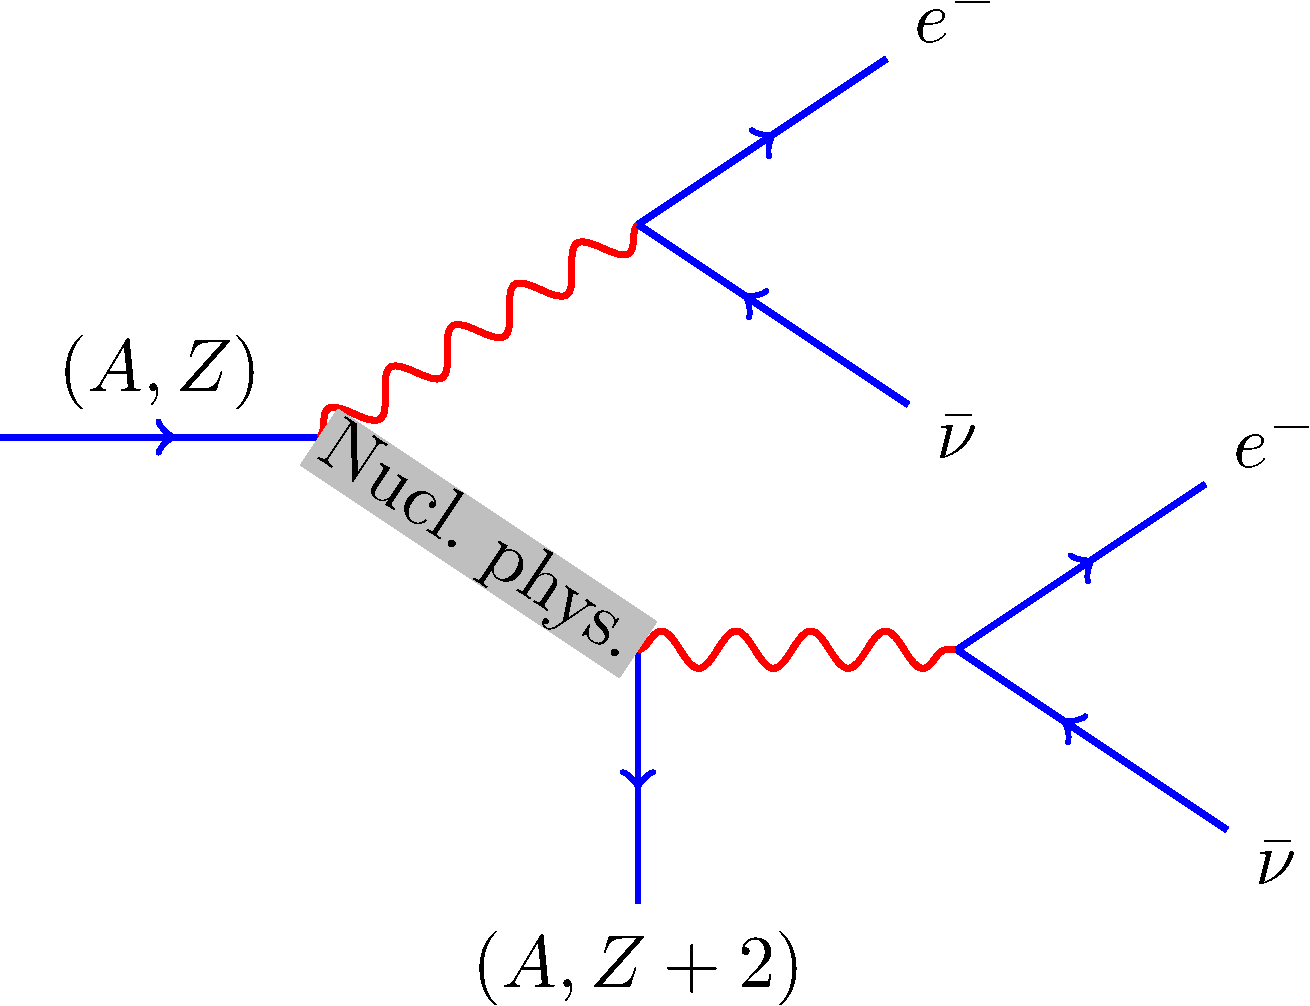
\includegraphics[height=\figheight]{2nubbDecay}
			}
			\subfigure[$\nonubb$]{
				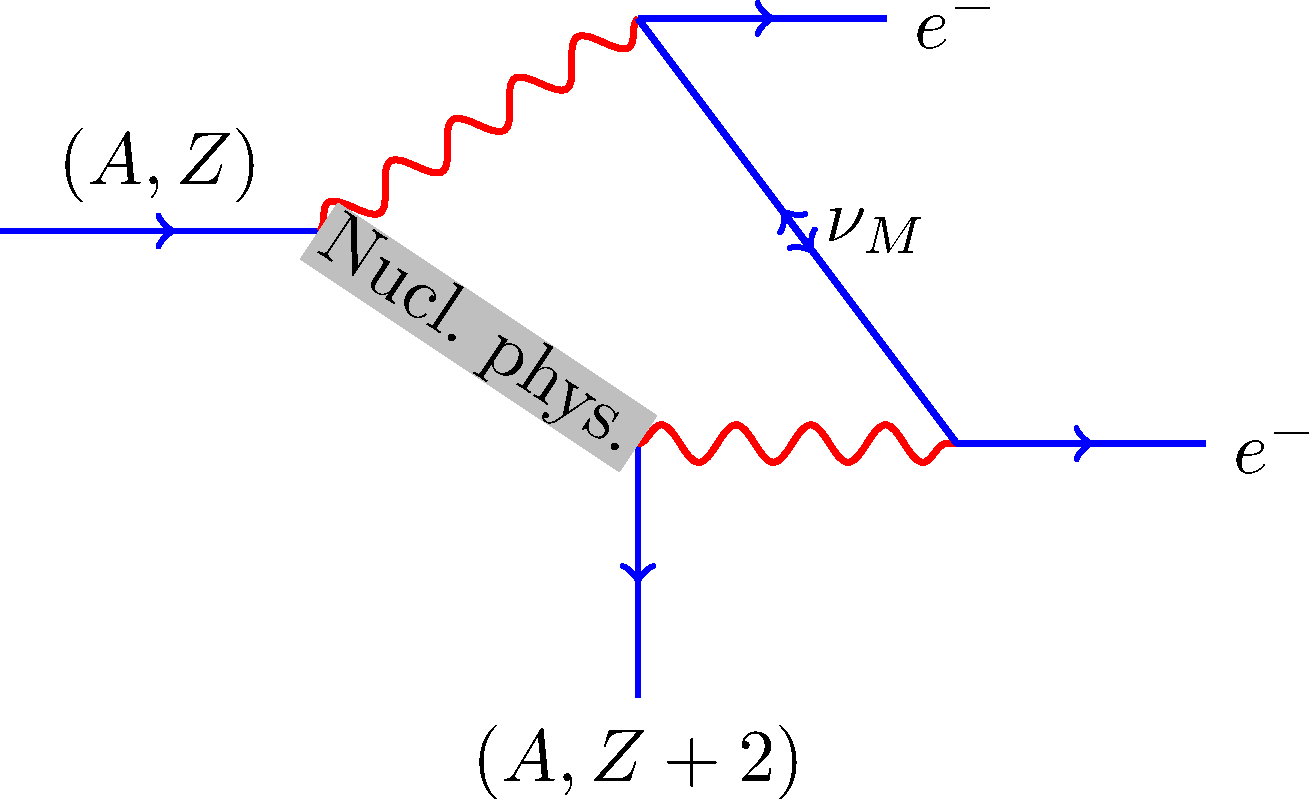
\includegraphics[height=\figheight]{0nubbDecay}
			}
		\caption[Schematic of $\twonubb$ and $\nonubb$ decays.]{Schematic figure of the two types of double-beta decay, 
		the 2$\nu$ mode and the 0$\nu$ mode.  
			In this schematic, the 0$\nu$ mode is mediated through the exchange of a virtual Majorana neutrino, $\nu_{M}$.}
		\label{fig:DBDK}
		\end{figure}
 

	
	\section{The \MJ\ Experiment}
	\label{sec:MJExperiment}
	
The search for a rare process such as $\nonubb$ necessarily involves maximizing the magnitude of the expected signal while
simultaneously reducing backgrounds that may mimic the sought-after process.  
The \MJ~experiment proposes to search for $\nonubb$ in \gersevensix~using high-purity
germanium as both source and detector, thereby maximizing a possible signal from $\nonubb$. 
The first stage of this experiment will involve the deployment of 20-40~kilograms of germanium in an arrayed fashion in a \minmod~module with the goal to determine
the feasibility of scaling up to the 1-tonne scale.  To achieve this, the \MJ~experiment seeks to demonstrate less than
1~background count per year per tonne of enriched material in the
region-of-interest, a $\sim4$~keV window around the $\beta\beta$-decay
Q-value of $^{76}$Ge (2039~keV).  Low-capacitance, low-noise p-type point-contact (\ppc)
detectors will be deployed in these modules to take advantage of characteristics which make 
them beneficial for rare-process searches in general and for looking for $\nonubb$ in particular.  These characteristics and other details about \ppc~detectors will be discussed in Section~\ref{sec:PPCDets}.  

To achieve its background goals, the \MJ~experiment will employ standard
techniques for background reduction including: creation of detector mounts,
cryostats, and other components close to the detectors using ultra-clean
electroformed copper and other radiopure materials; use of passive shielding
against external radiation including a lead shield for gamma radiation and a
borated polyethylene shield for the moderation of cosmic-ray-induced neutrons;
use of active shielding (vetos) against cosmic-ray muons; and deployment of the
module underground in the Sanford Underground Lab at Homestake, South Dakota,
for moderation of cosmic-ray muons.  Engineering drawings given in
Figures~\ref{fig:MJEngDrawing1} and~\ref{fig:MJEngDrawing2} show both the
cryostat design and the expected shield construction, and indicate the modular
design of the experiment; additional, independent cryostats may be deployed
within the same shield geometry.  
% FixME update
The expected sensitivity of this first stage, 
assuming 3 years with 30~kg of enriched material or 90~kg-yr of $^{76}$Ge
exposure, is T$_{1/2}\geq 10^{26}$.  
%Further information on the
%\MJ~experiment can be found in technical documents \footnote{Available:
%http://majorana.npl.washington.edu/general.php}. 

	
		\begin{sidewaysfigure}
			\centering		
			\def\figheight{0.45\textheight}
			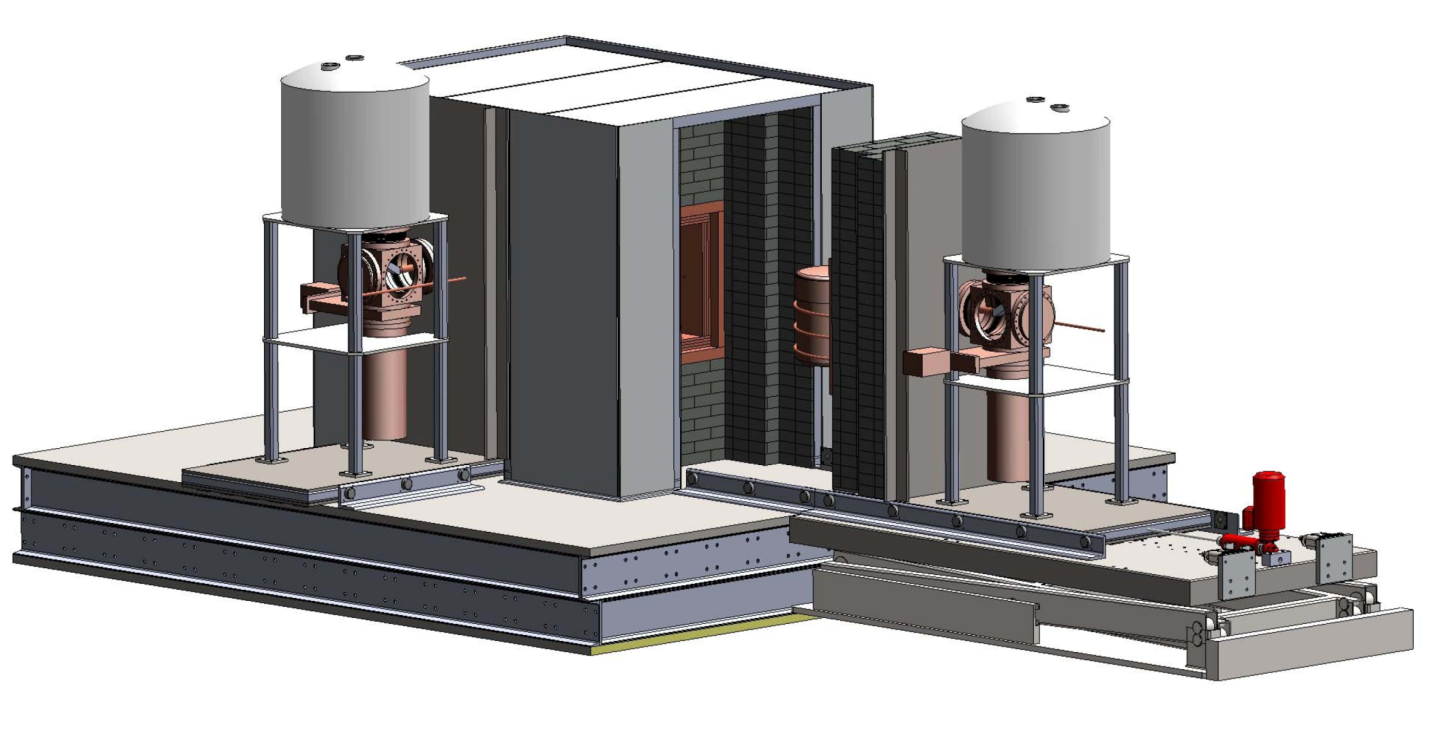
\includegraphics[height=\figheight]{ShieldDesign}
			\caption[\MJ~\minmod~shield geometry]{\MJ~\minmod~shield geometry.  The modular design of the shield will 
			enable a phased deployment of cryostats, allowing sets of detectors to be easily added after initial commissioning of the 
			experiment.  From the \MJ~collaboration~\cite{MJCollaboration}.}
			\label{fig:MJEngDrawing2}
		\end{sidewaysfigure}
	
		\begin{figure}
			\centering		
			\def\figheight{0.45\textheight}
			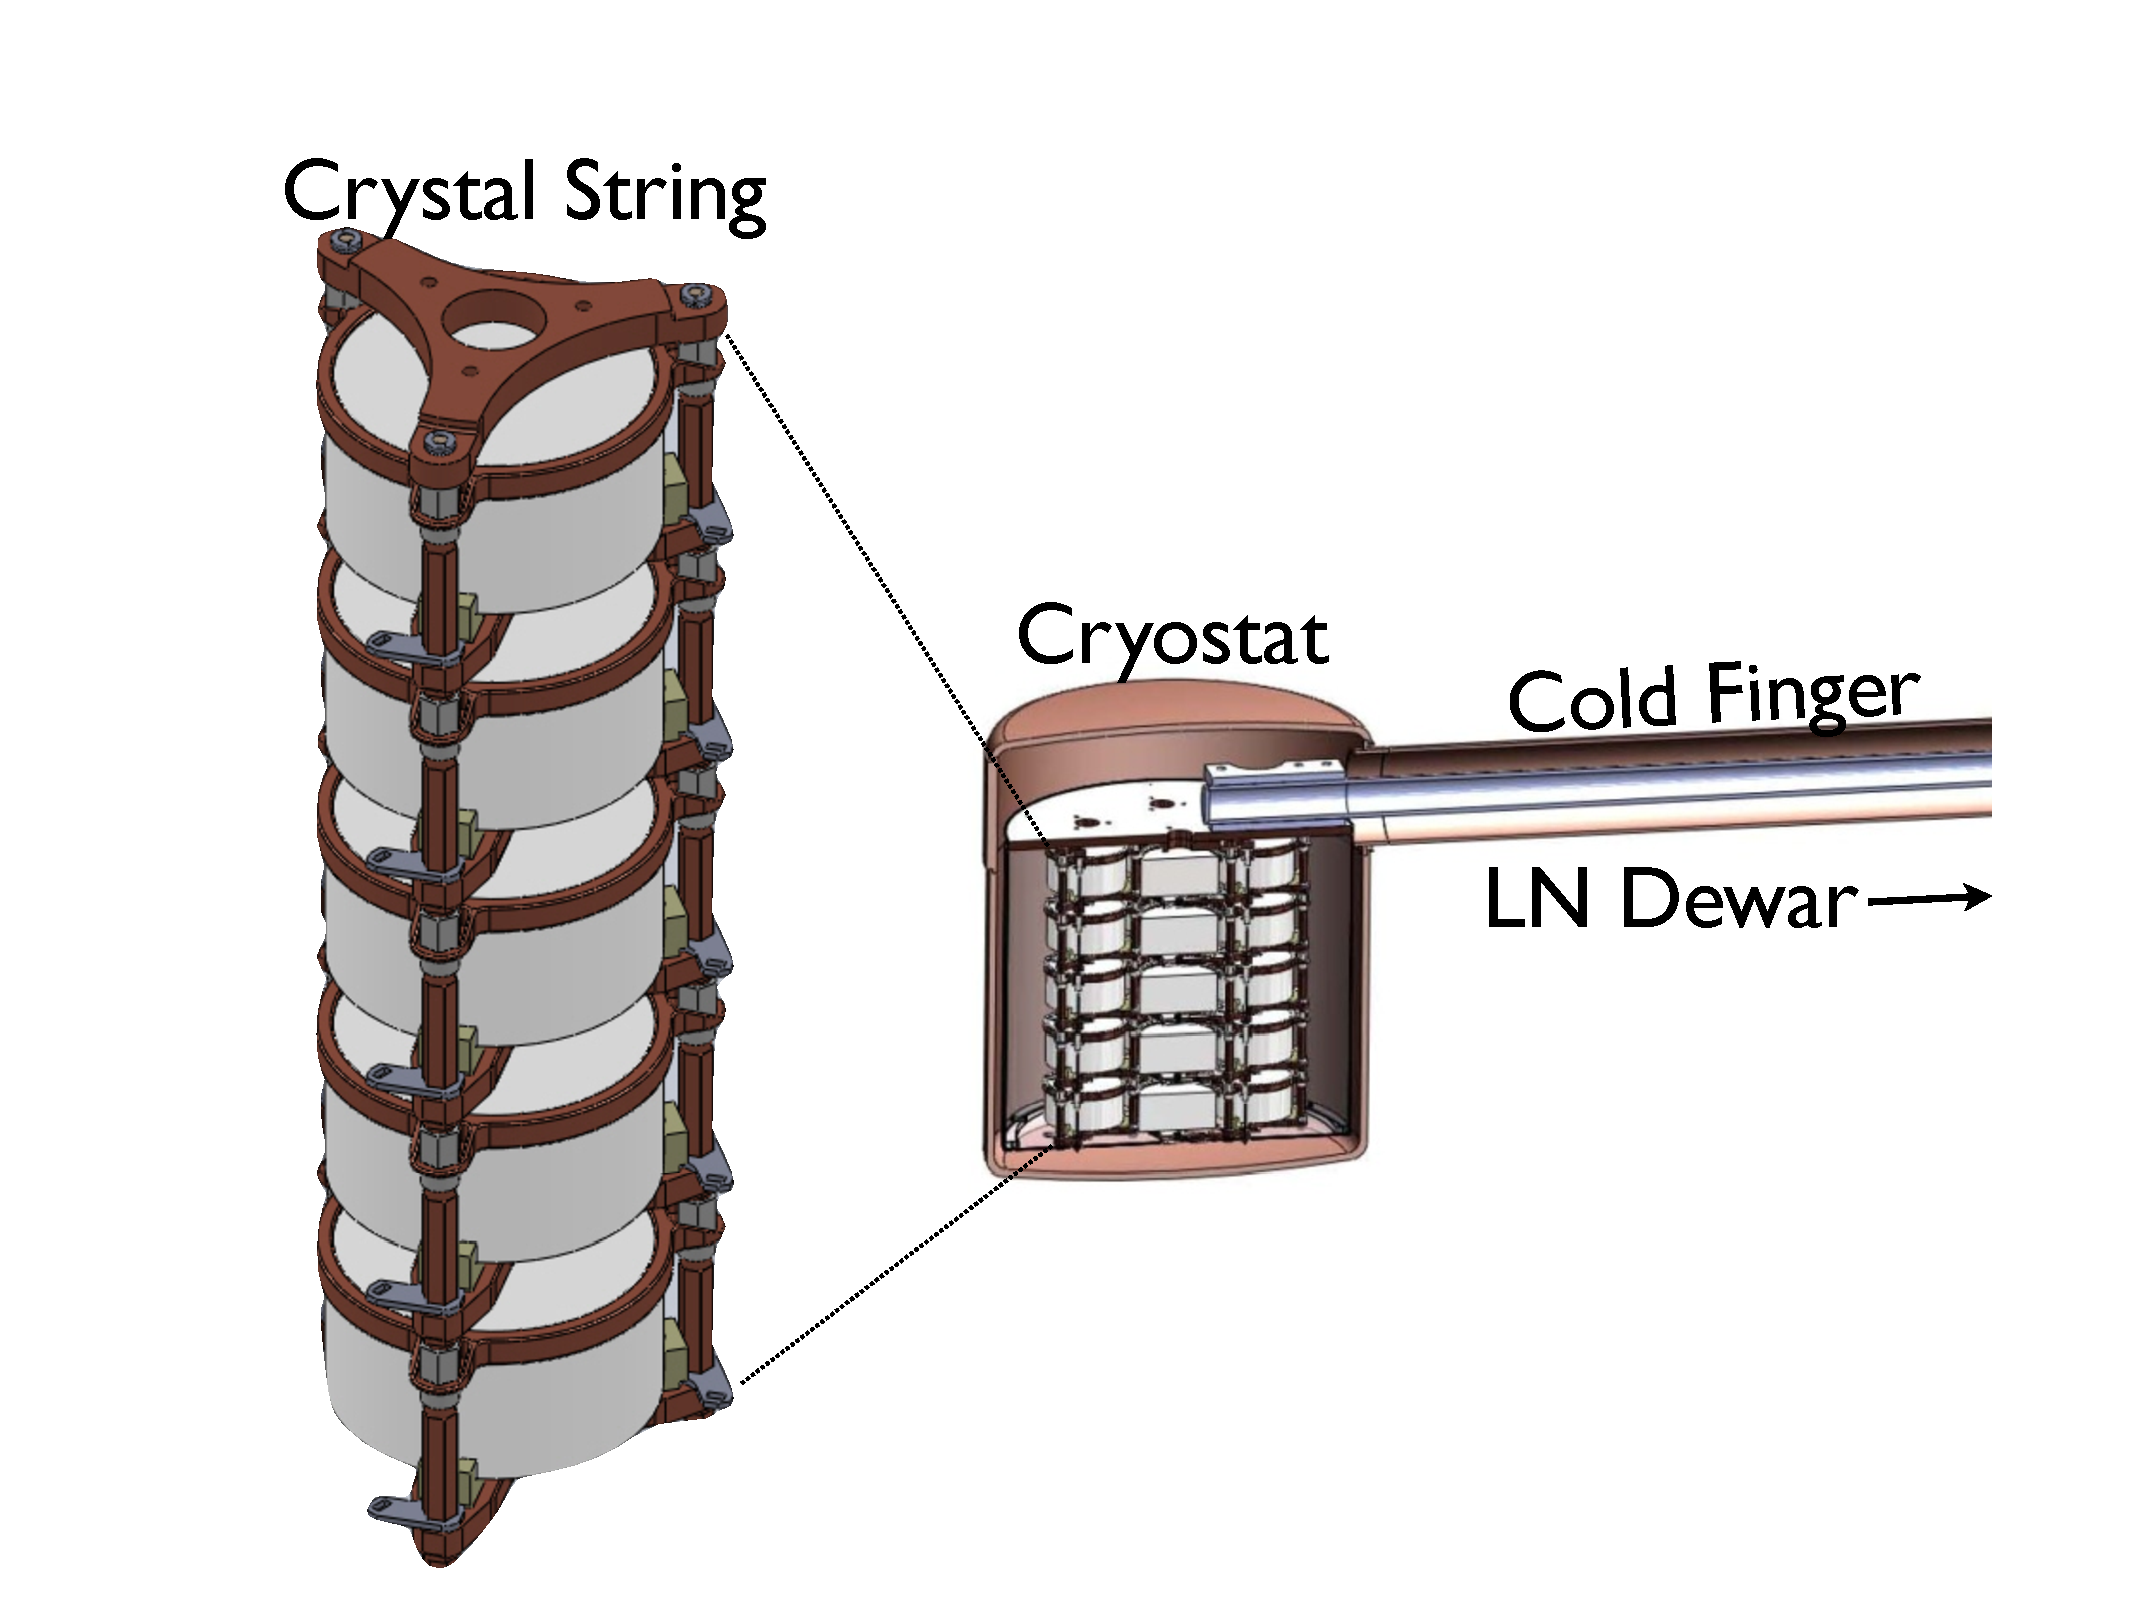
\includegraphics[height=0.79\textwidth]{CrystalCryostatDesign}
			\caption[\MJ~\minmod~cryostat and crystal string geometry]{\MJ~\minmod~cryostat and crystal string geometry, each
			crystal string houses 5~p-type point-contact germanium detectors.  From the \MJ~collaboration~\cite{MJCollaboration}.}
			\label{fig:MJEngDrawing1}
		\end{figure}

	
	\section{P-type Point-contact (\ppc) Germanium Detectors}
	\label{sec:PPCDets}

  P-type point-contact (\ppc) germanium detectors are an exciting detector
technology whose characteristics provide powerful tools in the search for
$\nonubb$ and enable searches for other rare physics processes at low energy, e.g.~dark matter.  
The electrode geometry of \ppc~detectors significantly reduces the
capacitance, reducing the energy threshold and enhancing the detector's
ability to detect low-energy ($O(100~\text{eV})$) processes.  Figure~\ref{fig:PPCGeom} shows a picture of the geometry of this detector in comparison to a standard semi-coaxial crystal.  In addition to improving the electronic response of the detector, the crystal geometry also yields a weighting field strongly peaked at the readout electrode (see e.g.~Figure~1 in~\cite{Ren10}).  This means that as charge drifts to the p contact after being created from energy deposition in the crystal (e.g.~from a physics interaction), no signal will be induced in the contact until the drifting charge is very near (within $\sim1$~cm of) the contact.  Additionally, charge drift times are increased by the longer drift paths.  These two characteristics coupled together improve the ability to distinguish between charge originating from one point in the crystal or from multiple sites in the detector.

An n-type detector with a point-contact geometry was developed by Luke et
al.~in 1989, demonstrating detector capacitance on the order of
1~pF~\cite{Luke89}.  With such a low capacitance and therefore a low-energy
threshold this detector was seen as a potential tool for dark matter detection, but this detector 
exhibited poor energy resolution due to incomplete charge collection attributed to charge-trapping effects.  
		\begin{figure}
			\centering
			\subfigure[Point-contact geometry.]{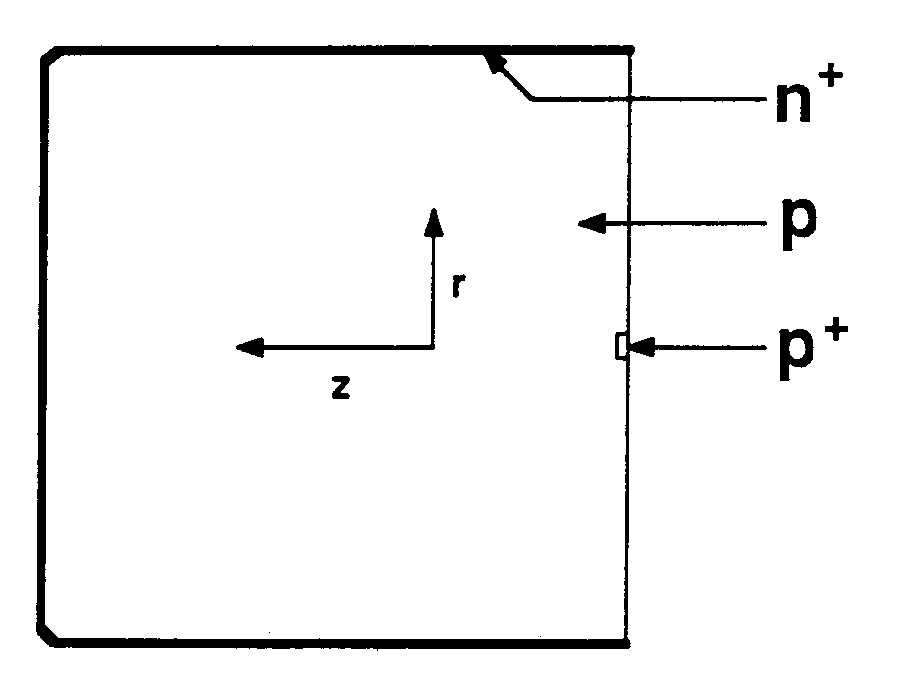
\includegraphics[height=0.2\textheight]{LukePPC}}
			\subfigure[Semi-coaxial geometry.]{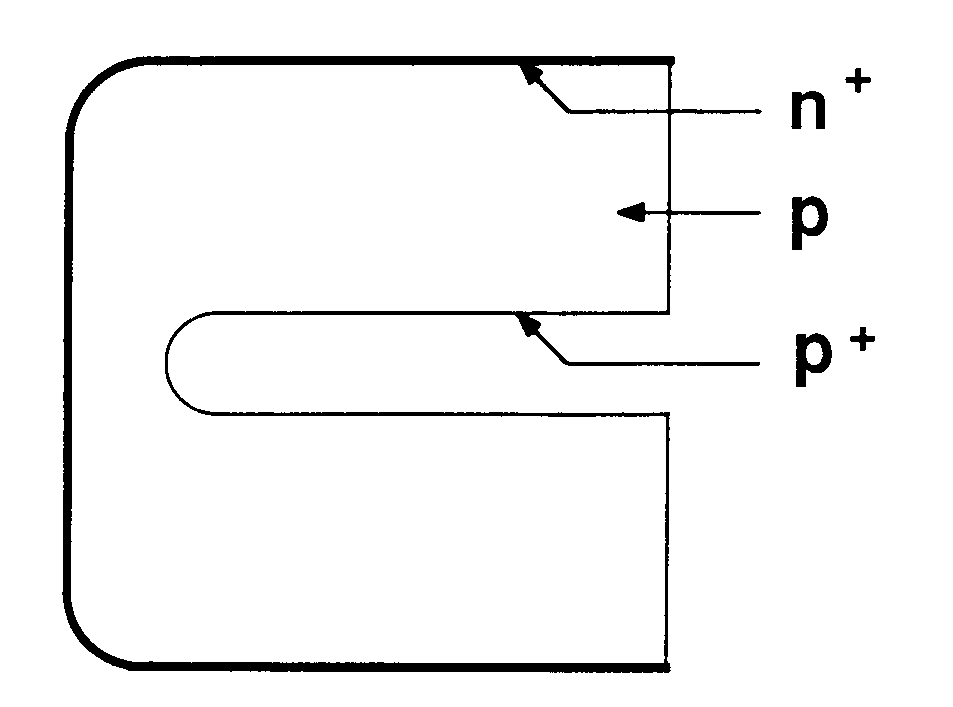
\includegraphics[height=0.2\textheight]{LukeCoax}}
			\caption[Ge detector geometry comparison: \ppc~and semi-coax.]{The left figure depicts the point-contact geometry, the right figure a conventional 
			         semi-coaxial geometry.  Figure adapted from~\cite{Luke89}.  The small diameter of the p contact in the
			          \ppc~detector reduces the capacitance of the detector improving the intrinsic noise characteristics.}
			\label{fig:PPCGeom}
		\end{figure}
  In 2007, Barbeau et al.~presented a new detector with a point-contact 
geometry, departing from previous convention by creating it out
of p-type material~\cite{Barb07}.  The reason for this
change was to take advantage of the reduced sensitivity of p-type crystals to electron trapping in germanium.  
Because p-type crystals collect holes instead of electrons at the p contact of the crystal, they are less likely to 
see a degradation of signal from electron trapping~\cite{Hull:2005p2207}.
With these changes, Barbeau et al.~demonstrated
a resolution comparable to conventional semi-coaxial germanium detectors and
an energy threshold of 330~eV making them an excellent candidate for double-beta decay searches.  
Other work with these detectors has supported these conclusions (see e.g.~\cite{Hull:2008p2206,Aalseth:2008aa}).
%Additionally, using a collimated $^{241}$Am gamma source (59.5~keV), they demonstrated differences in pulse rise-times based upon position of interaction (see Figure~\ref{fig:MeasPulses}).   

%\begin{figure}
%\begin{center}
%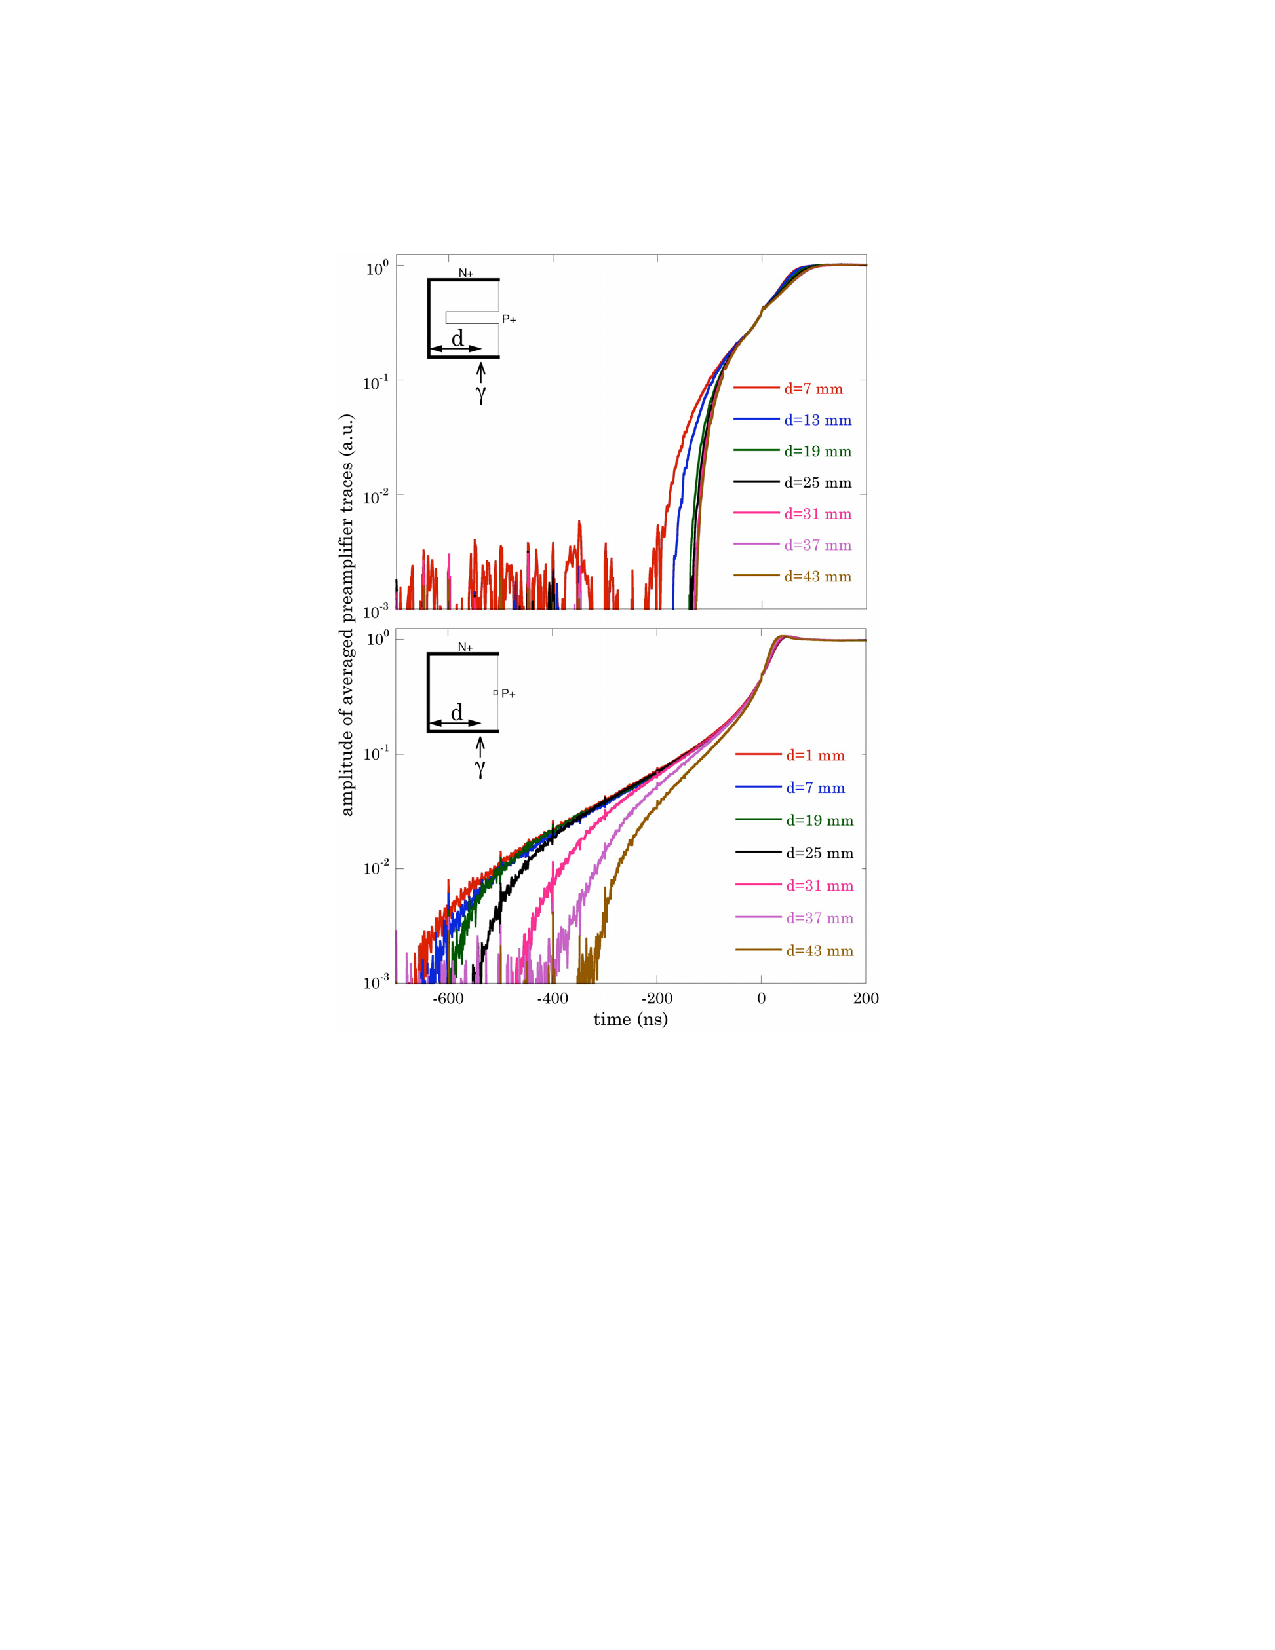
\includegraphics[width=0.8\textwidth]{BarbPPC}
%\caption{Pulses from a collimated ${241}$Am gamma source incident upon the surface
%         of a conventional semi-coax detector (top) and a p-type point-contact (bottom).
%         The expansion of the charge collection time in the \ppc~detector versus
%         the conventional semi-coax detector is evident.  (Figure from~\cite{Barb07}.)}
%\label{fig:MeasPulses}
%\end{center}
%\end{figure}

	\section{\ppc~Detectors for the \MJ~Experiment}

For the proposed \MJ~experiment, the characteristics of the \ppc~detector
will aid in the reduction of backgrounds and in enhancing the physics reach of
the experiment.  Since $\nonubb$ is an inherently single-site event, cutting out
multi-site events during data analysis provides a powerful background reduction
tool.  For conventional semi-coaxial detectors, various tools have been developed
to tag multi-site events based upon the shape of the measured pulse (see,
e.g.~\cite{Aal00}).  The expansion in time
of charge collection in \ppc~detectors makes distinguishing multi-site events easier and improves the efficiency for single-site acceptance vs. multi-site rejection of a pulse-shape analysis routine (see~\cite{Budjas:2009zu,Ren10}).

To improve the bandwidth of the detector readout it is necessary to
place front-end preamplification electronics (e.g.~field-effect transistors) nearby the detectors
inside the detector cryostat.  As with any low-background 
experiment the increase of material (and especially material close to
sensitive detectors) introduces potential radioactivity that could
increase background.  The single-contact nature of the \ppc~requires only one
front-end per crystal, thus reducing the material inside the cryostat and possibly
softening radiopurity requirements.

Cosmogenically-produced $^{68}$Ge is a significant background
source for the \MJ~experiment, decaying first via electron capture to $^{68}$Ga
(T$_{1/2}=271$~d) and then to $^{68}$Zn (Q=2921~keV, T$_{1/2}=68$~m).  The
initial decay is characterized by the emission of Auger electrons and/or soft x-rays
summing to the orbital energy of the captured electon (e.g.~1.3~keV for L-capture, 10.3~keV for K-capture) 
and it is possible to use these to tag the $^{68}$Ge decay.  A time cut can then be introduced to veto events
occurring within a few $^{68}$Ga lifetimes to mitigate background from that
decay without seriously affecting detector live time.   \ppc~detectors have an
improved sensitivity to low-energy physics because of their low noise and 
low-energy threshold and so should significantly enhance the tagging of the
$^{68}$Ge decay.  

Though characteristics of \ppc~detectors will prove useful in searching for
$\nonubb$, the low-energy threshold will also
expand the physics reach of the \MJ~experiment.  Access to low energies will 
make the \minmod~sensitive to low-energy nuclear recoils and enhance its capacity as a dark matter
detector.  The functionality and usefulness of the \ppc~detector as a tool for dark
matter searches is considered in much more detail 
throughout the remainder of this dissertation.


%The low energy threshold and low noise of the \ppc~detector won't necessarily
%improve a search for $\nonubb$ since the region-of-interest for $^{76}$Ge is at
%2039~keV, well above the energy region where electronic noise and detector
%capacitance dominate the overall noise.  

%An additional advantage of the \ppc~detectors, as with other p-type
%detectors, is its thick outer Li contact which tends to be on the order of
%$\sim0.5$~mm.  Alpha particles emitted from Rn daughters contaminating the
%surface of cryostat components in the \MJ~demonstrator module might provide
%a significant background source (see e.g.~\cite{Joh07}).  However, the outer
%Li contact of a p-type detector renders much of the outer surface insensitive
%to these decays.  Additionally, the outer contact improves the robustness of
%the surface making the detector less susceptible to damage during
%handling.  This is an important consideration especially for detectors 
%designed to be installed in an arrayed fashion.  

	\section{Searching for Dark Matter: Low-energy Physics with \ppc~Detectors}
	
		\subsection{Evidence for Dark Matter}
	% Galactic rotational curves
	From cosmological observation there exists significant evidence that the matter density of the universe is mostly composed of non-luminous, gravitationally-interacting particles referred to as `dark matter'.  Perhaps the most convincing and intuitive empirical indications arise from measurements of galactic rotational curves.  Astronomers have measured the rotational velocity of stars in galaxies and determined the relation of this velocity versus the radial distance from galactic center.  When the rotational velocity is compared to that expected given the observed radial distribution of mass, it is found that galaxies are rotating much more quickly than they should be.  Essentially, there is simply not enough observable mass to explain why the galaxies' rotational velocities do not tear them apart.  This realization indicated that some other mass must exist to hold the galaxies together, and that this mass was hidden due to its weak or nonexistent coupling with photons.  Such a weak interaction with electromagnetism would make the dark matter unsusceptible to frictional forces and also would make it non-luminous or `dark.'  By including a mass density of dark matter in a `dark matter halo' around galaxies, astronomers could successfully reproduce observed rotation curves.  An example of such a rotational curve and a three-component fit (visible matter (e.g.~stars), gas, and dark halo) has been included from Reference~\cite{Begeman:1991iy} in Figure~\ref{fig:DMRotCurve}.

		\begin{figure}
			\centering
			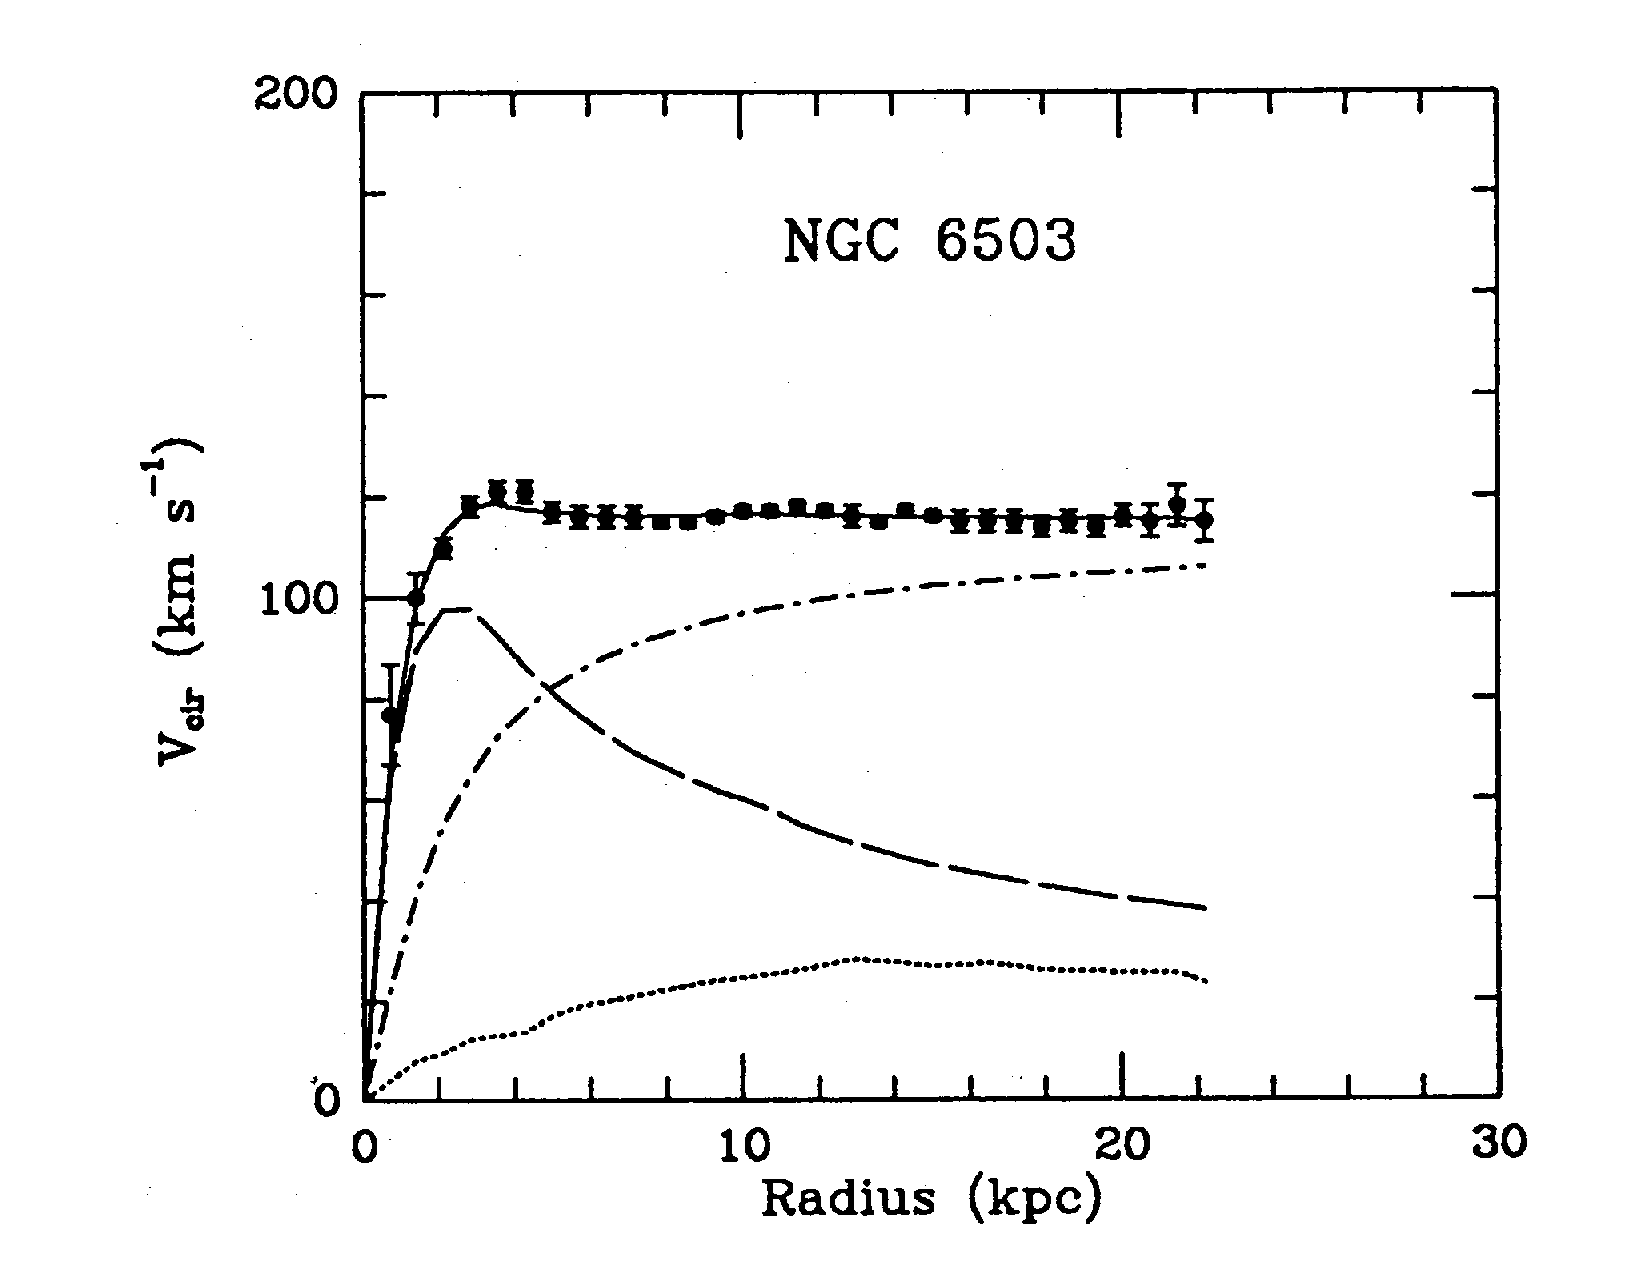
\includegraphics[height=0.45\textheight]{DMRotationalCurves}
			\caption[Galactic rotational velocity curve of NGC 6503.]{Galactic rotational velocity curve of NGC 6503
			from~\cite{Begeman:1991iy}.  The solid line is a three-component fit to the data with components from:
			visible mass (dashed), gas (dotted) and the dark halo (dash-dot).  }
			\label{fig:DMRotCurve}
		\end{figure}
	% WMAP results (large-scale structure)
	Other evidence of dark matter comes from measurements of large-scale structure through the analysis of the anisotropy of the cosmic microwave background (CMB) (see e.g.~\cite{Amsler20081}).  The extraction of cosmological parameters (e.g.~total matter density, baryon density, Hubble parameter, etc.) occurs by fitting the CMB data using model-based assumptions.  In particular, the parameters-of-interest are the total matter density, $\Omega_{m}$, and the baryon density, $\Omega_{b}$, which have been measured to be (in units of critical density):
		\begin{eqnarray*}
			\Omega_{m} & = & 0.256 \pm 0.02 \\
			\Omega_{b} & = & 0.044 \pm 0.003~\cite{Amsler20081}
		\end{eqnarray*}
If baryonic matter composed the majority of the mass in the universe, one would expect these two quantities to be equivalent.  Instead, the significant discrepancy between the two indicates the presence of unaccounted for material.  Therefore, the dark matter component is the difference between these two components: $\Omega_{dm} = \Omega_{m} - \Omega_{b} = 0.21 \pm 0.02$, indicating a large proportion of dark matter in the universe on the order of 20\%.

	% Bullet cluster
	
	Perhaps the most visually stunning evidence for dark matter comes from the
`bullet cluster' (galactic cluster 1E 0657-56)~\cite{Clowe06}.  In this
particular example two subclusters have collided with one another $\sim$100~Myr
ago, subjecting the contents of each to frictional forces.  The stars and
galactic components of the subclusters were scarcely affected due to their relatively wide spacing, passing by
one another and interacting largely only gravitationally. However, the trajectories
of the hot gas making up the majority of the subclusters' baryonic mass density
were significantly altered.  The matter density of the gas component was
measured using images from the Chandra x-ray observatory and the total mass
density of the cluster was measured using gravitational lensing.  When plots of
these measurements are superimposed (see Figure~\ref{fig:DMBulletCluster}
from~\cite{Clowe06}), it is clear that the two centers (of each subcluster) of
the total mass density are offset from the centers of the gas-plasma mass
density.  This indicates the presence of non-luminous (dark) matter that 
interacts weakly with both the normal baryonic matter and with itself.  
	
			\begin{figure}
				\centering
				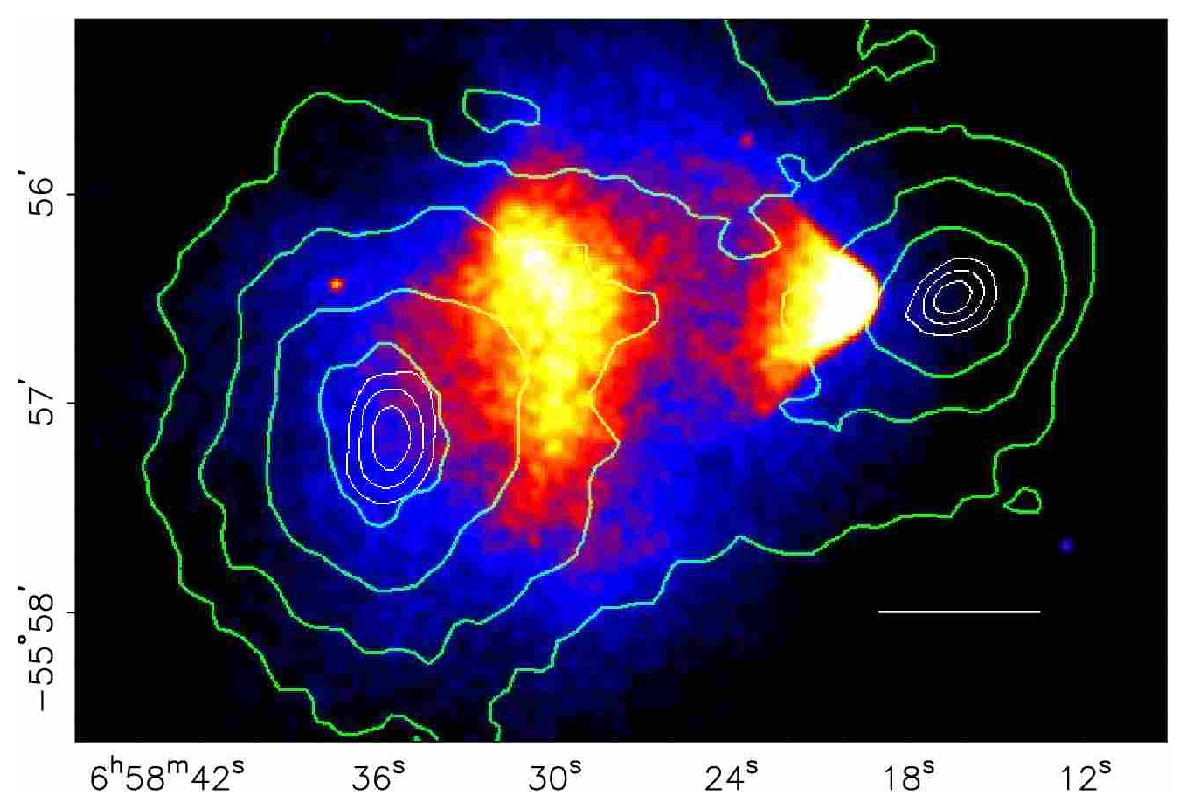
\includegraphics[height=0.45\textheight]{BulletCluster}
				\caption[Mass and x-ray image of the `bullet cluster', galactic cluster 1E 0657-56.]{Mass and x-ray image of 
				galactic cluster 1E 0657-56, 
				the `bullet cluster'.   The total mass, denoted by contour lines, has been measured using gravitational lensing; 
				the density of the gas, which composes the majority of the baryonic matter density in the cluster, has been 
				imaged using the Chandra x-ray observatory.  %The displacement of the centers of the total mass 
				Figure taken from reference~\cite{Clowe06}.}
				\label{fig:DMBulletCluster}
			\end{figure}	
	
	% Dark matter candidates	
		\subsection{Dark Matter Candidates}
	
	Whereas there are many particle candidates for dark matter, they share several general qualities:

	
	% Properties of dark matter particles
	% Stable
	% Interact poorly (or not at all) with electromagnetism
	% Should be non-relativistic (cold)
	
			\begin{enumerate}	
				\item Stable, having lifetimes at least on the order of the age of the universe.  Otherwise, dark matter would have
				decayed away.  
				\item Poor or no interaction with electromagnetism, making them non-luminous or `dark'.
				\item Non-relativistic at the time of galaxy formation: `hot' dark matter would move too quickly to clump, 
				not allowing it to affect large-scale structure formation as required by cosmological observation.  
			\end{enumerate}		

	% Looking at two species in particular:
	% WIMPs
	% Argument for WIMP dark matter: abundance considerations, freeze-out condition
Additionally, dark matter will compose a halo in our galaxy which the earth passes through as it transits around the sun.  Therefore, depending on the velocity dependence of the dark matter interaction and the velocity distribution of WIMPs in the galactic halo, it is possible that the earth's orbit can generate an annual modulation in the dark matter signal, providing an additional distinguishing characteristic.  In the following, we will consider two potential species of dark matter in particular: WIMPs and axions. 
			\subsubsection{WIMPs}
 WIMPs, or Weakly-Interacting Massive Particles, (denoted from here on by $\chi$) are more of a class of candidate particles than one in particular, defined by the fact that these types of particles predominantly (or exclusively) interact via the weak force.  Several reviews outline in more detail the characteristics of WIMP particles, see e.g.~\cite{Jun96,Lew96}.  An argument for the existence of WIMPs relates to how they can `naturally' explain the dark matter relic abundance.
 % while making a few assumptions.  
  For example, during the period right after the big bang as the temperature of the universe was still quite hot, WIMPs would have been in equilibrium with other fermions, undergoing annihilation and generation according to the two-way reaction: $\chi\bar{\chi} \leftrightarrow f\bar{f} $ (see e.g.~Figure~\ref{fig:WIMPExampleProduction}).  As the temperature of the universe cooled below the mass of $\chi$, eventually this two-way process would shut off in one direction allowing only the interaction $\chi\bar{\chi} \rightarrow f\bar{f} $ to remain.  At this point in time, the rate of decay of $\chi$ has been calculated to be $\Gamma_{\chi} = \WIMPAnn n_{\chi}$~\cite{Jun96}, where $\sigma_{A}$ is the average cross-section for $\chi$ to annihilate into lighter fermions, $v$ is the average particle velocity, and $n_{\chi}$ is the density of WIMP particles.  The expansion of the universe would then reduce the density of $\chi$s, effectively shutting off this annihilation process and `freezing out' a so-called relic abundance of the particles.  

An estimate of the density of this abundance remaining today times the Hubble constant squared, $h^{2}\sim0.5$, can be calculated (see, e.g.~\cite{Jun96}):
			\begin{eqnarray}
				\Omega_{\chi} h^{2} & = & (2.6 \times 10^{-10}~\text{GeV}^{-2})~\WIMPAnn \\
				%\WIMPAnn & \sim & \frac{\alpha^{2}}{M_{\text{weak}}^{2}} \sim 10^{-9}~\text{GeV}^{-2}\\			
			\end{eqnarray}
and if we assume that this interaction follows the weak force, we can estimate the average cross section times the velocity as:
			\begin{eqnarray}
				%\Omega_{\chi} h^{2} & = & (2.6 \times 10^{-10}~\text{GeV}^{-2})~\WIMPAnn \\
				\WIMPAnn & \sim & \frac{\alpha^{2}}{M_{\text{weak}}^{2}} \sim 10^{-9}~\text{GeV}^{-2}\\			
			\end{eqnarray}
which leaves us with an estimate of 	$\Omega_{\chi} h^{2} \sim 0.2$, close to the observed cold-dark-matter density.  This realization has not been interpreted as a `coincidence' and instead is suggested as compelling support for the possibility of WIMP existence~\cite{Feng20052}.  
		
			\begin{figure}
				\centering
				\def\figheight{0.4\textwidth}
				 \subfigure[WIMP annihilation and production] {
				 	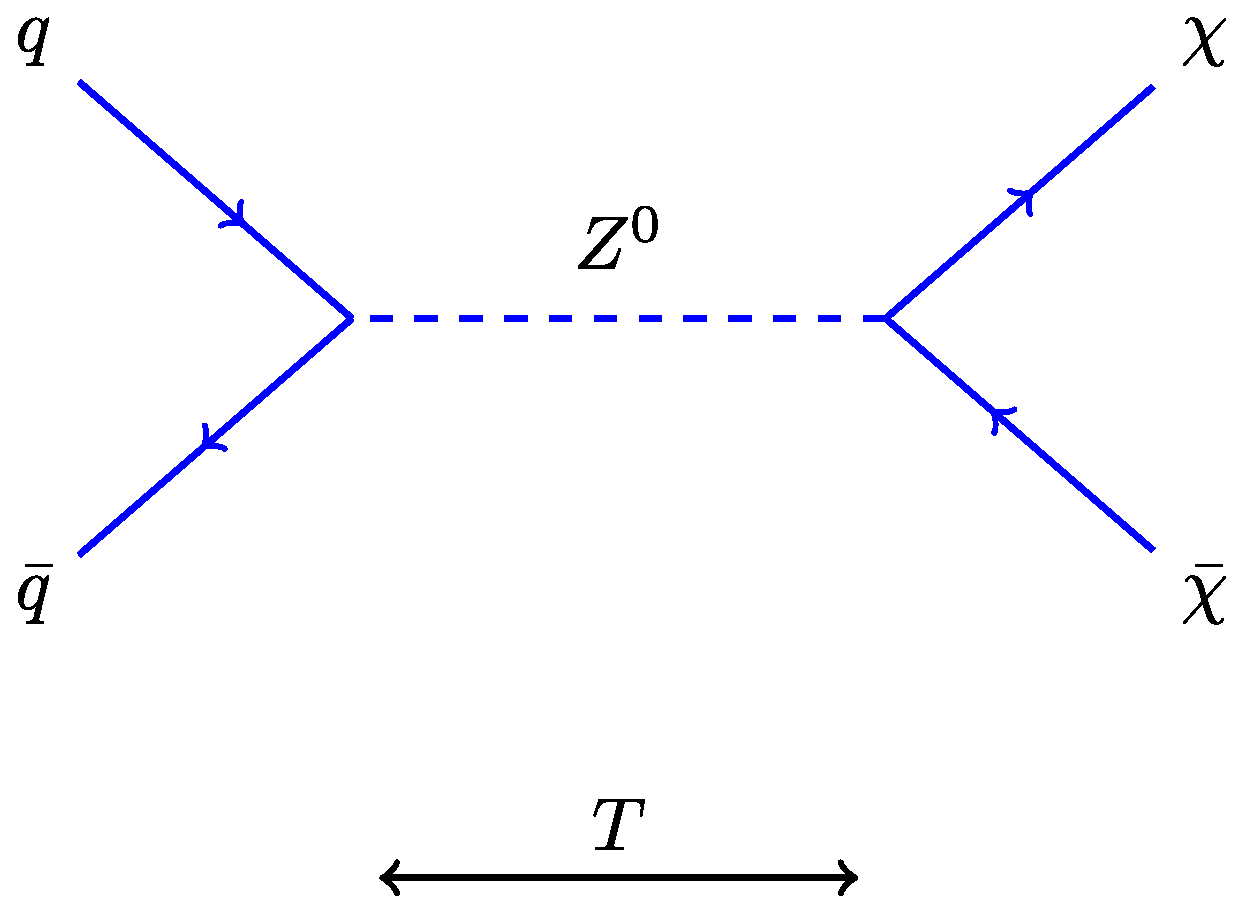
\includegraphics[width=0.6\textwidth]{WIMPProduction}
					\label{fig:WIMPExampleProduction}
				}
				\subfigure[WIMP elastic scattering]{
					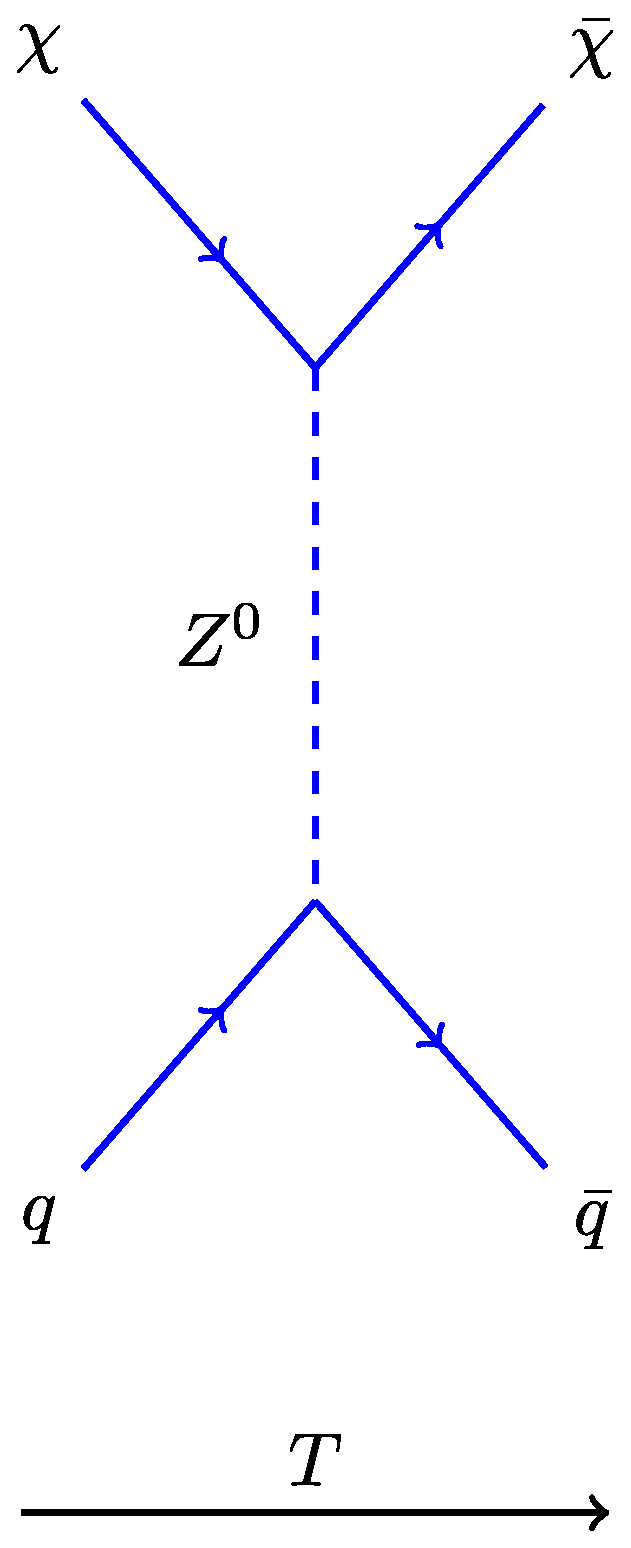
\includegraphics[width=0.25\textwidth]{WIMPScattering}
					\label{fig:WIMPExampleScattering}					
				}
				\caption[Relevant WIMP-quark interactions during hot and cold universe epochs.]{Example WIMP-quark 
				interactions mediated by the exchange of a $Z^{0}$ boson with the direction
				of time, $t$, indicated for each at bottom.  The left figure is applicable for WIMPs undergoing annihilation and 
				generation during the equilibrium phase at
				the beginning of the universe, when the temperature of the universe was much greater than the mass of $\chi$.
				The right figure denotes a mathematically equivalent interaction, an elastic-scattering process
				of $\chi$s off quarks becoming relevant as the temperature of the universe reduced below the mass of $\chi$.}
				\label{fig:WIMPExample}
			\end{figure}	
			
	The direct detection of WIMPs is possible via their elastic scattering off fermions, see e.g.~Figure~\ref{fig:WIMPExampleScattering}.  In creating a
detector, we are of course generally limited to composing it out of electrons,
neutrons, and protons.  In principle, WIMPs could scatter off any fermion
sharing a coupling to a mediating boson, but the kinematics of such a
non-relativistic recoil maximize the energy transfer when the target particle
has mass comparable to that of the incident particle.  In the case of WIMPs
with hypothesized masses $\sim1\to1000$~GeV, an energy transfer is maximized
during coherent recoil off a nucleus having similar or equal mass.
Additionally, WIMP scattering off bound electrons is suppressed due the mass
ratio $m_{e}/m_{\chi}$, as well as the small size of the electronic wave
function (see e.g.~\cite{Kopp09}) making the nuclear recoil the expected
primary method of detection.  The standard form of the energy spectrum for a
WIMP-induced nuclear recoil is outlined later in
Section~\ref{sec:CalcLimitsOnWIMPSignal}.
	
			\subsubsection{Axions}
			\label{sec:AxionsAsDM}
	% Axions
	% Arguments for axions:
	% pseudoscalar bosons
	% Peccei-Quinn model - preserve CP in QCD 
	
	Axions are light, pseudoscalar bosons that were originally suggested as a
mechanism to solve the CP problem of Quantum Chromodynamics (QCD)~\cite{Pec77}.  In particular, the QCD
Lagrangian includes a CP-violating term: \[
			\mathcal{L}_{\Theta} = \bar{\Theta} \frac{\alpha_s}{8 \pi} G^{\mu \nu a} \tilde{G}_{\mu \nu}^{a}
			\]
where $\bar{\Theta}$ is an angle with possible value between $-\pi$ and $\pi$.  The lack of experimental evidence for CP violation in QCD suggests that this value is very small or 0, an `unnatural' solution given its range of possible values.  The Peccei-Quinn mechanism was proposed~\cite{Pec77} to explain this issue by adding an additional $U(1)_{PQ}$ symmetry to the Lagrangian.  The breaking of this symmetry results in a Nambu-Goldstone boson -- the axion -- updating the CP-violating portion of the QCD Lagrangian to be:
			\[
			\mathcal{L}_{\Theta} = \left( \bar{\Theta} - \frac{\phi_{A}}{f_{A}}\right) \frac{\alpha_s}{8 \pi} G^{\mu \nu a} \tilde{G}_{\mu \nu}^{a}
			\]	
with $\phi_{A}$ the axion field and $f_{A}$ the axion decay constant~\cite{Amsler20081}.  The expectation value of the axion is found to be $\phi_{A} = f_{A} \bar{\Theta}$ thereby directly canceling the CP violating term.  Further detail regarding axions can be found in several current reviews, including~\cite{Amsler20081,2008LNP}.
	
	Bounds on axion properties can derive from cosmological observations as well as direct experimental searches.  For example, cosmological data can constrain axion models by looking for the evidence of additional unexplained energy loss in stars (see, e.g.~\cite{Gondolo09,Raffelt95}).  Direct detection measurements may take advantage of axions coupling with 2~photons, looking for their interaction in high-intensity magnetic fields, as is the case with the CAST experiment~\cite{Arik09} searching for axions produced in the sun, or searching for an axion interaction in a resonant microwave cavity within a magnetic field, as does the ADMX experiment~\cite{Asz10}.  Germanium detectors are not ideal for searching for such a signal, but can put bounds on the strength of the axion's coupling with electrons by searching for the inelastic scattering of an axion off an electron.  This interaction and the observed signal is discussed in more detail in Section~\ref{sec:CalcLimitsOnHeavyAxionSignal}.
		
		\subsection{\ppc~Detectors and Dark Matter}

	
	% WIMPs, truncated exponential
	
	\ppc~detectors can provide excellent dark matter detectors due to their low-energy threshold ($O(100~\text{eV})$) and excellent resolution down to threshold.  This can be made more clear if we consider the signal that WIMPs and axions can leave in a germanium detector.  These signals and their exact spectral form are discussed in more detail later for WIMPs (see Section~\ref{sec:CalcLimitsOnWIMPSignal}) and axions (see Section~\ref{sec:CalcLimitsOnHeavyAxionSignal}), but we consider their general properties here.  For a more complete reference on the direct detection of dark matter, see~\cite{Gaitskell:2004fk}.
	
	The nuclear recoil signal from a WIMP is essentially described as an exponential in energy space truncated by the finite escape velocity of the WIMP from the halo (see, e.g.~\cite{Jun96, Lew96}).  The exponential constant is determined by the mass of the WIMP and the spectrum becomes steeper as the mass gets smaller.  This can be visualized in Figure~\ref{fig:WIMPDiffMasses}.  It is clear that lowering the threshold of the germanium detector is critical to detecting low-mass WIMPs, due to the steepening of the curves and the truncation of the signal.  The sub-keV thresholds of \ppc~detectors therefore enables sensitivity to these low masses.  Most WIMP experiments rely on the ability to distinguish between electron and nuclear recoils for background reduction since the vast majority of backgrounds (e.g.~gammas, alphas, and betas) interact solely with electrons.  \ppc~detectors will be unable to distinguish between these two types of events, instead relying on the passive reduction of radioactivity through the choice of radiopure materials and appropriate shielding.
	
			\begin{figure}
				\centering
				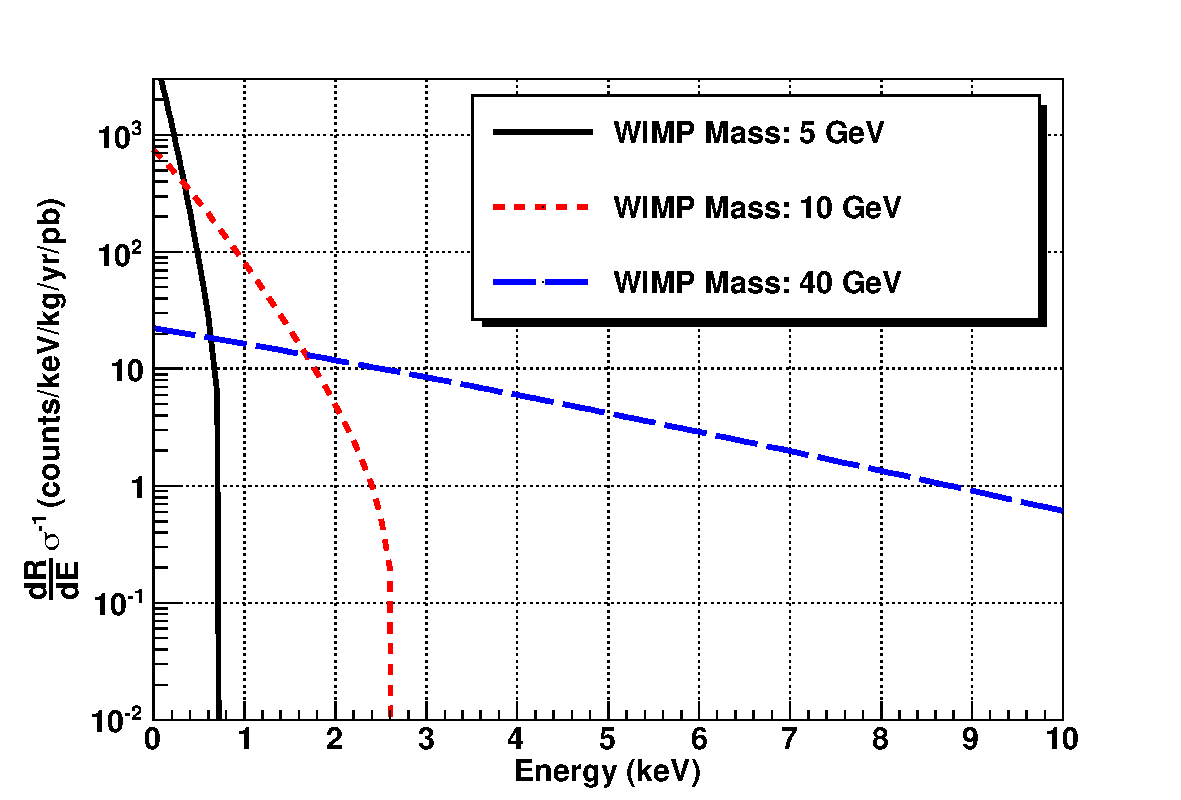
\includegraphics[width=0.9\textwidth]{WIMPModelCompareDiffMasses}
				\caption[Ionization spectrum of a WIMP nuclear-recoil in a Ge detector.]
				{Ionization spectrum (differential rate vs.~energy) of a WIMP
				nuclear-recoil in a Ge detector normalized by the interaction cross section.
				The signal becomes steeper with lower WIMP mass and the truncation due to the
				escape velocity is more apparent at low mass.  Because of the characteristics
				of the signal, for example, a germanium
				  detector with threshold greater than 1~keV could not detect a recoiling WIMP of mass 5~GeV, underscoring
				  the need for low thresholds to detect low-mass WIMPs.}
				\label{fig:WIMPDiffMasses}
			\end{figure}

	% Axioelectric effect - gaussian signal

	The signal for a non-relativistic axion interacting via the axioelectric effect has been derived in~\cite{Pospelov:2008jk}.  This particular inelastic interaction involves the deposition of the \emph{complete} energy of the axion, yielding an electron-recoil signal centered at the mass of the axion.  The low noise of \ppc~detectors yields excellent sensitivity to non-relativistic axions with masses $\leq10$~keV due their sharp resolution at low energies.  This enhanced performance is especially clear when compared to the capabilities of NaI scintillation detectors.  A comparison of an axioelectric signal at a defined axion-electron coupling ($\gaa$) is provided in Figure~\ref{fig:ResCompare} for characteristic resolutions of NaI and germanium detectors.  In this plot, it is clear that the improved resolution of the germanium detector allows less smearing of the signal, yielding more counts in a narrower peak.  This enhanced resolution enables superior distinction of the signal in the presence of background.
	
		\begin{figure}
			\centering
			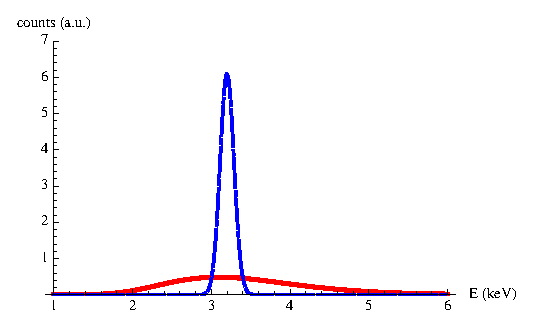
\includegraphics[width=0.9\textwidth]{DAMARes}
			\caption[Axioelectric signal at $m_{a}$ = 3.2~keV]{Axioelectric signal at $m_{a}$ = 3.2~keV comparing 
			the detector responses of germanium (blue, dashed) and NaI (red, solid) assuming some axion-electron coupling $\gaa$.  The resolution functions ($\sigma(E)$) for Ge and NaI are $\sqrt{(0.0697)^{2} + (0.3)(2.96\times10^{-3})E}$ and
			$(0.448/\sqrt{E} + 0.0091) E$ with $E$ in keV, from~\cite{Aalseth:2008aa} and~\cite{Bernabei2008297} respectively.} 
			\label{fig:ResCompare}
		\end{figure}
	
	It is important to note that \ppc~detectors do not search for any specific signal other than energy deposition in the crystal.
Because of this, they may be sensitive to interactions of particles not yet theorized or not yet recognized as theoretically 
well motivated.  Therefore, these detectors provide a necessary complementarity to those experiments looking for particular types
of signals and will widen the experimental landscape essential for the development and constraint of theories pertaining to dark matter.

	\section{Outline of this Dissertation}

		% Development of a digital DAQ, understanding the needs to get a fully-functional DAQ able to satisfy both the requirements of nonubb and low-energy physics
		% Deployment of an initial detector and system underground, what we learned
		% A final system (with updated DAQ, etc.) underground
		% Limits on WIMPs and the axioelectric effect as well as considerations for Majorana

	This dissertation will focus on understanding and exploiting the low-energy
capabilities of \ppc~detectors.  %It will begin by considering the data
%acquisition (DAQ) needs to read out these detectors to enable full access to
%physics at $\qval$ and at low energies.  
It will begin by describing the application of a digital data acquisition
system to a \ppc~detector deployed underground at Soudan Underground Laboratory
in Soudan, Minnesota, and outline conclusions from this initial study.  Results
and knowledge gained from this initial detector were then applied to the
deployment of another, lower-background \ppc~at Soudan.  The analysis of this
detector, including the generation of limits for WIMP and axion dark matter,
comprises the bulk of the thesis.  Finally, the work ends with some contextual
discussion of these results, focusing on estimating the sensitivity of the
\MJ~\minmod~to detect dark matter.  Appendices detailing the development and
use of DAQ hardware and DAQ and analysis software for the results of this
dissertation are included for reference.
 
\clearpage

% ========== Chapter 2

% In this chapter, I will describe the techniques used to characterize the BeGe detectors,
% including tests involving e.g. resolution, noise, charge collection, multi-site rejection.
%
% Results of the tests will be presented
%
% It is also possible to present some of my hardware/software development work here
% since this is relevant to the characterization studies.  I imagine these
% generally will occupy appendices.

\chapter{Development of a Digital Data Acquisition System for P-type Point Contact Detectors}
\label{chap:DAQDevel}
	\section{Introduction} 
	
	The detectors in the \MJ~\minmod~will be readout using a digital data acquisition system using fast ADCs to digitize raw preamp traces to be used in later pulse-shape analysis.  The requirements of a digital DAQ system for the \minmod~were investigated, in particular focusing on refining the hardware specifications needed to achieve the physics goals of the project.  These specifications must be sufficient to achieve two general goals: (1) background reduction through pulse-shape analysis, especially in the $\nonubb$ region-of-interest, and (2) low-energy performance enabling both background reduction at $\qval$ and sensitivity to low-energy physics (dark matter).  
	
	 This chapter focuses on investigations of several issues of the DAQ:
		\begin{itemize}
			\item Sampling rate 
			\item Operational stability
			\item Low-energy performance
			\begin{itemize}
				\item Triggering
				\item Low-energy resolution
			\end{itemize}	
		\end{itemize}
but does not detail the development of all the hardware and software to run most of these tests.  For more information regarding that work, please see Appendix~\ref{app:ORCASoftwareChapter}.  Chaper~\ref{chap:DeploymentPPC2Soudan} describes efforts to test elements of the DAQ systems presented here in a deployed, underground environment.

	Because P-type Point Contact detectors will be used in the \MJ~\minmod, it was necessary to use such a detector for these tests.  A \ppc~detector (henceforth referred to as \ppc2) was procured by PNNL in January 2008 to be used in studies aimed at more clearly understanding the detector technology~\cite{Orr2007}.  Initial tests took place in the laboratory, focusing on basic operation and pulse-shape analysis techniques relevant for background reduction in the $\nonubb$ region-of-interest and for Dark Matter searches~\cite{Orr2008}, including results presented here (see Section~\ref{sec:HeadToHeadCompare}).  Following these tests, in November 2008 the detector was deployed underground at Soudan National Laboratory at a depth of 2100~m.w.e.~to investigate both the low-energy performance and operational stability.
	   
	\section{Baseline DAQ system}

	The baseline system for development used the Gretina Mark IV digitizer designed by the GRETA collaboration~\cite{Anderson:2009p1293}.  This VME64x-based ADC digitized 10 independent channels at 100~Ms/s with a resolution of 14 bits.  The card was read out using the ORCA DAQ software developed at the University of Washington and at the University of North Carolina (\cite{ORCA}, see also Appendix~\ref{app:ORCASoftwareChapter}).  
	
	\section{Digitizer comparison tests}
     	\label{sec:HeadToHeadCompare}
     	% Comparison between 100 MS/s and other cards.
	
	Since the Gretina card had been determined as a candidate card for the \MJ~\minmod, head-to-head tests between it and digitizers with different characteristics was necessary.  The purpose of these measurements was to investigate how the specifications of each digitizer affected its ability to perform pulse-shape analysis for background reduction through multi- and single-site event selection.  The decided method was to take data from \ppc2 concurrently with different digitizers using a $^{232}$Th source.  $^{208}$Tl, a daughter in the thorium chain, produces a double-escape peak (DEP) at 1592.5~keV which is predominantly composed of single-site events and is commonly used (e.g.~\cite{Abt2007332,Orrell:2007tt}) to test pulse-shape analysis algorithms.  After taking concurrent data, it was planned to process the waveform data with the same algorithm to see how each digitizer performed.
	
		\subsection{Measurement}
	     	\label{sec:HeadToHeadCompareMeasurement}     
	The measurement with \ppc2 took place at Pacific Northwest National Laboratory running a round-robin test with 3~different digitizers, two cards at a time.  The digitizers used were the Gretina Mark IV, XIA DGF4-c, and the XIA Pixie-4, details about which are given in Table~\ref{tab:HeadToHeadComparisonDetectorChars}.  The \ppc2 preamp had two identical signal outputs, and so each of these was AC-coupled to one of the two digitizers being used for each test.  The inhibit output, which generated a logic pulse when the reset circuitry of the preamp was active, was split and input in to each digitizer.  The time signature of the inhibit pulse was later used to synchronize the data sets (see Section~\ref{sec:HeadToHeadCompareAnalysis}.  
	
	The DAQ software used for both XIA cards was an IGOR Pro-based package designed and shipped by XIA.  	The setup for the Gretina card was similar but simpler to that described in Section~\ref{sec:DeploymentPPC2SoudanDAQSystem}, again using ORCA to readout the card.  The data from each DAQ system were converted to a common format and stored in ROOT files using MGDO data objects.  More details on ORCA and MGDO can be found in Appendices~\ref{app:ORCASoftwareChapter} and~\ref{app:MGDO}.  Each XIA card was run in parallel with the Gretina card and around 2~hours live-time of source data was taken for each pair, though the wall clock time was roughly 2 (4) times this during runs with the DGF4-c (Pixie-4) due to induced deadtime.  (The Gretina card is designed to be deadtime-less.)  
		
			\begin{table}
				\centering
				\begin{tabular}{l|c|c|c}
					Name & Sampling Rate & Bit Resolution & Form Factor \\
					\hline
					XIA DGF4-c & 40 Ms/s & 14 bits & CAMAC \\
					\hline
					XIA Pixie-4 &  75 Ms/s & 14 bits & PCI \\
					\hline
					Gretina Mark IV &  100 Ms/s & 14 bits & VME64x \\										
					\hline					
				\end{tabular}
				\caption[Comparison of digitizer characteristics]
				{Comparison of digitizer characteristics used in this test.}
				\label{tab:HeadToHeadComparisonDetectorChars}
			\end{table}	
		
		\subsection{Analysis}
	     	\label{sec:HeadToHeadCompareAnalysis}     		
		 % Synchronizing two systems is the basic idea here, go over how this is actually done
	The data were converted to the ROOT-based MGDO format using the OrcaROOT processing libraries.  The amplitudes of each Gretina pulse were calculated using an offline trapezoidal filter.  The value of the onboard trapezoidal calculation was used for each XIA card.  Once converted, the runs with each pair of cards were synchronized together using the timing of the inhibit pulse.  The basic algorithm searched for common time differences between reset pulse events, accommodating the fact that the XIA cards tended to miss numbers of these events given their dead-time and that their 32-bit on-board clocks rolled over more often than the 48-bit clock on the Gretina card.  Once a catalog of synchronized events was determined, the data were compiled into a single set of ROOT files for later pulse-shape analysis.  An example of a synchronized event is shown in Figure~\ref{fig:HeadToHeadPulseExample}.  The difference in decay time constants is due to the different input impedances of each card.  (Same-valued capacitors were used to AC couple each card.)  The synchronization between the two cards ensured that each event processed was generated by the same physics event.
	
			\begin{figure}
				\centering
				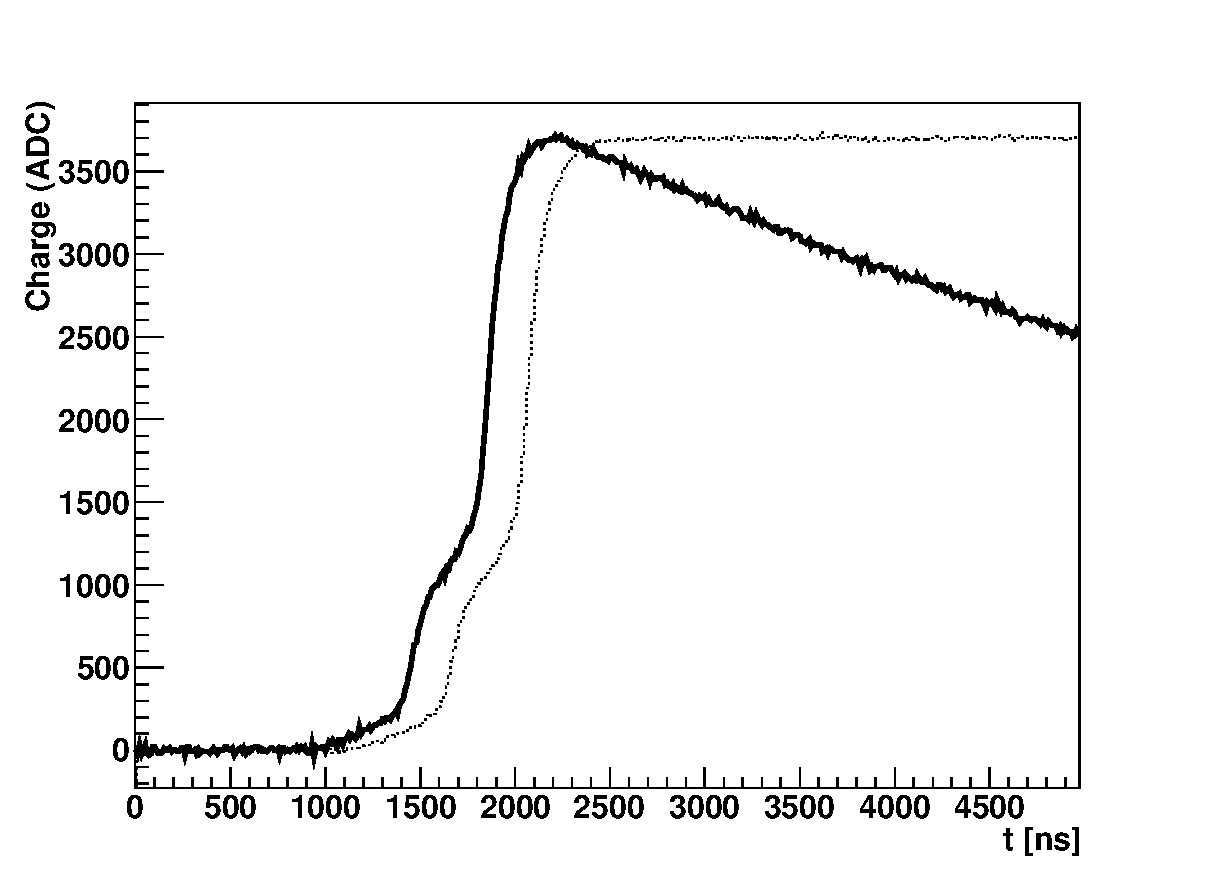
\includegraphics[width=0.9\textwidth]{PPC2WaveformComparison}
				\caption[Visualization of synchronized pulses from the Gretina and Pixie digitizers]
				{Visualization of two synchronized pulses from the Gretina (bold) and Pixie digitizers.  
				The different decay constant are due to the different input impedances of each card.}
				\label{fig:HeadToHeadPulseExample}
			\end{figure}

	 After synchronization, a simple pulse-shape analysis algorithm~\cite{Budjas:2009zu} developed by the GERDA collaboration was applied to the data.  In this algorithm, the ratio $A/E$ is calculated, where $A$ is the maximum of the current pulse (derivative of the charge pulse) and $E$ is the amplitude (energy) of the charge pulse.  This ratio can then be used to discriminate between single- and multi-site events due to the fact that events with multiple interaction sites tend to have wider current pulses for a given energy, $E$.  A version of this algorithm was implemented using waveform processing code in MGDO.  
	 
	 Before processing, the data sets were reduced to include only events in a $\sim$50~keV window around the $^{208}$Tl DEP at 1592.5~keV.  For each event of this subset, the current waveform was generated by using a Savitzky-Golay derivative filter~\cite{Sav64aa} of size~5 and degree~4 and the current maximum was saved.  Cuts were then applied to the data for a range of values for $A/E$ and the data were fit using binned maximum likelihood using the RooFit toolkit~\cite{ver03aa} over the range $1570\to1615$~keV.  This fit was used to estimate the survival probability of the $^{208}$Tl DEP and background reduction in the continuum and nearby peaks, including the 1588.2 and 1580.5~keV gamma peaks of $^{228}$Ac.  An example of such a fit is shown in Figure~\ref{fig:HeadToHeadExampleFit}.  A direct comparison between the pairs of cards is possible by looking at the background reduction and survival probability versus the cut parameter, $A/E$, as calculate for each digitizer.  These results are shown for DGF4-c and Gretina cards in Figure~\ref{fig:HeadToHeadDGF4cResults}, and for the Pixie-4 and Gretina cards in Figure~\ref{fig:HeadToHeadPixie4cResults}.  It is clear from these plots that the 3 cards behave comparably with this particular algorithm.  The only discrepancy exists in the DGF4-c vs.~Gretina results: the DGF4-c has a slightly steeper acceptance curve around an $A/E$ value of 62.
	 
			\begin{figure}
				\centering
				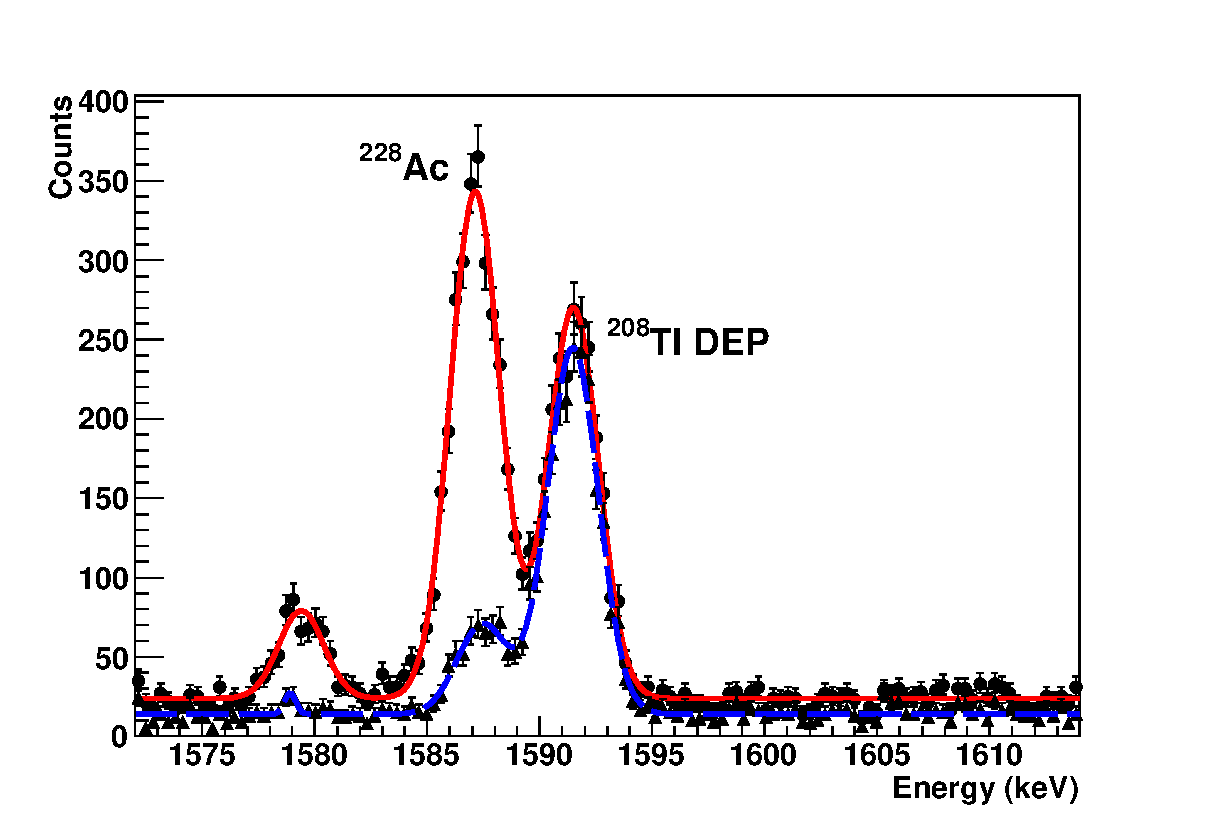
\includegraphics[width=0.9\textwidth]{Tl208DEPFitExample}
				\caption[An example set of fits using the Gretina card]
				{An example set of fits using the Gretina card.  The solid line (circles) is without cuts, the dashed (triangles)
				 with cuts, yielding a signal acceptance of $94.8\pm1.77\%$ in the $^{208}$Tl DEP and a $89.1\pm0.99\%$ 
				 reduction in the adjacent 1588.2~keV $^{228}$Ac peak.}
				\label{fig:HeadToHeadExampleFit}
			\end{figure}	
		
		% Then application of a simple PS analysis.  
			\begin{figure}
				\centering
				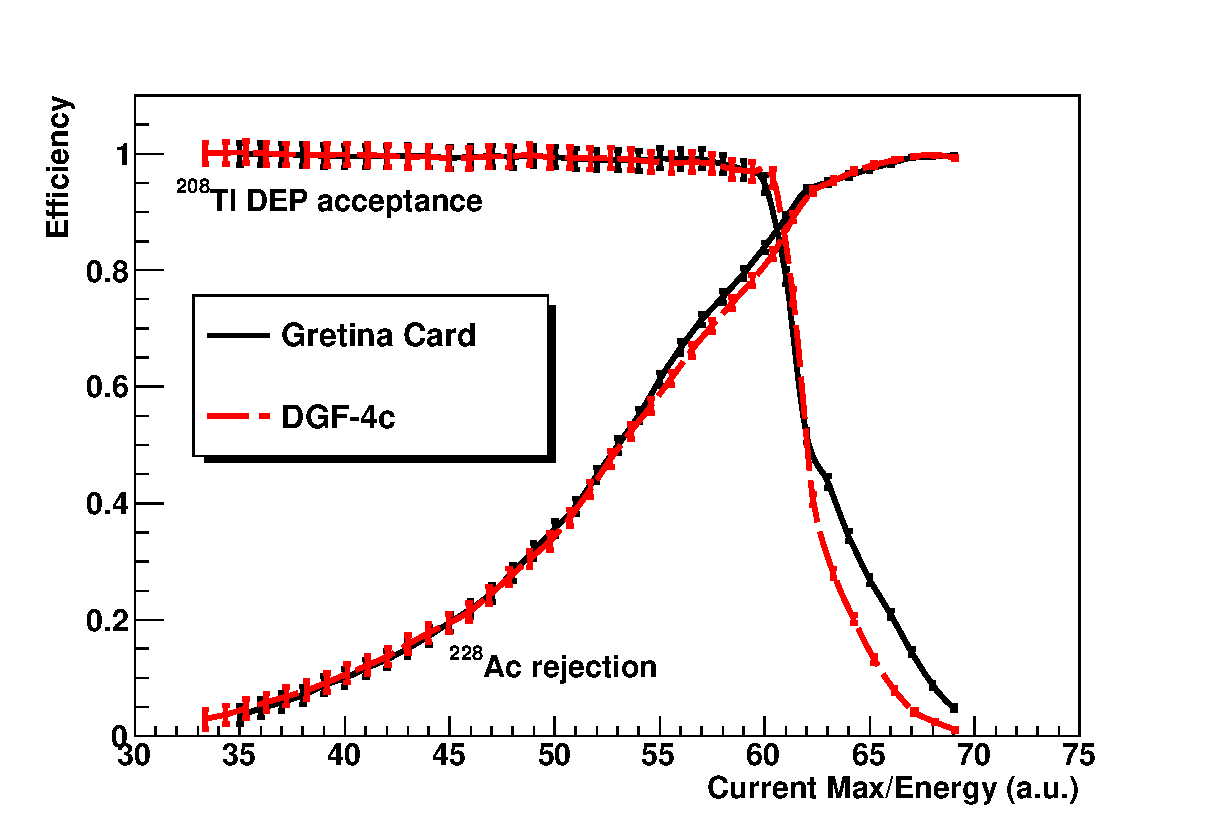
\includegraphics[width=0.9\textwidth]{DGF4c_Vs_Gretina}
				\caption[Cuts for Gretina vs. DGF-4c]
				{Cuts for Gretina vs. DGF-4c.}
				\label{fig:HeadToHeadDGF4cResults}
			\end{figure}	
	
			\begin{figure}
				\centering
				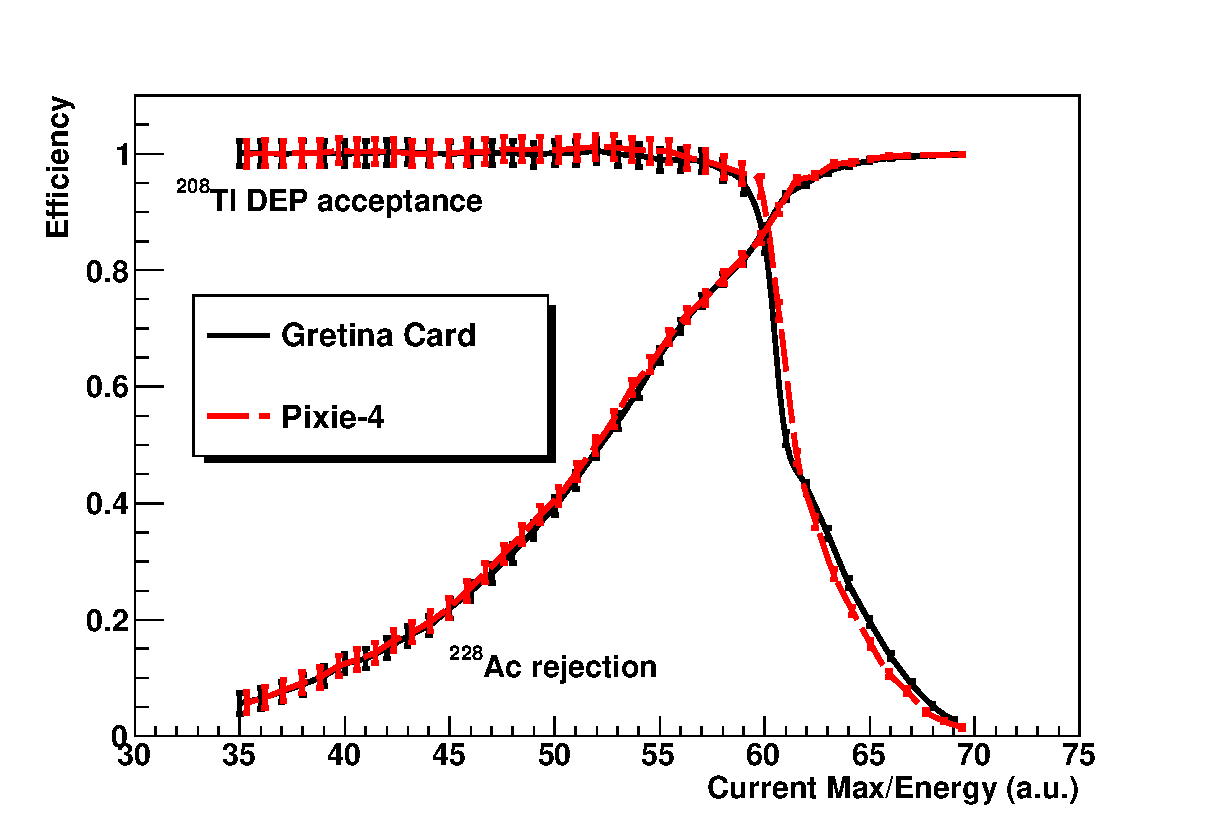
\includegraphics[width=0.9\textwidth]{Pixie_Vs_Gretina}
				\caption[Cuts for Gretina vs. Pixie-4c]{Cuts for Gretina vs. Pixie-4c.}
				\label{fig:HeadToHeadPixie4cResults}
			\end{figure}	
			
		\subsection{Conclusions}
	     	\label{sec:HeadToHeadCompareConclusions}
		
	For the simple pulse-shape algorithm presented here the 3 digitizer cards perform similarly, suggesting that the $A/E$ calculation is not significantly sensitive to the sampling frequency of the fast ADC.  More advanced PSA, such as those based upon comparing pulses to a library of single-site events~\cite{Ren10}, are more likely to depend on the sampling characteristics of the digitizer.  
		% Reference Ren's paper, a lot of work that has been done there, understanding that this 
		% is a very simple technique applied to data.     

	\section{Development and testing of the Gretina Mark IV digitizer}
		\subsection{Trigger Design and Tests}
		\label{sec:DeploymentPPC2SoudanTriggerDesign}     
			
	Before deployment of the DAQ system underground in Soudan, triggering tests were performed to determine the optimum conditions for minimizing the energy threshold of the electronics.  The goal of these initial measurements was also to develop an automated set of tests to perform regularly on \ppc2 \emph{in situ}.  The basic technique to measure the trigger efficiency of a system is to inject a pulse of known amplitude into the system near threshold and scan the amplitude of the pulse around that threshold.  One can determine the probability of detecting a pulse by either knowing the rate of the injected pulse and performing the test for a known period of time, or by having an independent measure of the the timing of the injected pulse (i.e.~a synchronization pulse) and performing a coincidence measurement.  For these tests, the latter method was chosen as it was deemed a cleaner technique to extract both the trigger efficiency given a certain pulse amplitude as well as the false trigger rate at a particular threshold setting.  
	
	The test setup included the pulser and computer-controlled attenuators described in Section~\ref{sec:DeploymentPPC2SoudanDAQSystem} and was run by the ORCA DAQ software.  To vary the amplitude of the injected pulse, it was decided to keep the output pulse from the waveform generator constant and change the attenuator settings.  Scripts were designed in ORCA to perform these variations automatically.  The attenuated pulse was amplified using a Phillips 777 before being injected directly into a Gretina card to ensure that the noise of the input signal dominated the intrinsic noise of the digitizer.  The amplitude of the measured pulse was estimated using an offline trapezoidal filter as was done in later analysis (see Section~\ref{sec:DeploymentPPC2SoudanAnalysis}).  Because a similar detector system to \ppc2 was unavailable above ground at the time of the tests, it was impossible to simulate the exact noise environment of \ppc2's electronics.  To circumvent this limitation, all the measurements were determined in terms of signal-to-noise ratios to be able to compare directly to the detector system.  For example, a measured signal-to-noise ratio could be multiplied by the separately measured magnitude of the detector noise to provide a rough calibration of the results.  Initial measurements quoted this value as 180~eV~FWHM\footnote{This value was measured using an analog shaping amplifier and is dependent upon the shaping times of the amplifier.  In practice, this value is different than one calculated using digital shaping (i.e.~with a trapezoidal filter, as was done in this analysis) and so was interpreted as an estimate when compared directly to digital measurements.}~\cite{Orr2007}.  
	
		Initial measurements found that the Gretina on-board trigger, a leading-edge discrimination (LED) differential algorithm with fixed shaping, achieved $\sim$90\% efficiency at an S/N of $\sim$6, suggesting that a similar efficiency would be found at $\sim$1~keV on the detector system.  This was at least a factor of 2 worse performance than demonstrated in analog readout systems with a detector of similar noise characteristics~\cite{Barb07}.  The degraded trigger performance was due to the limited shaping associated with the LED trigger which had not originally been designed to trigger on very-low-amplitude preamp signals.  To solve this issue, a hybrid digital/analog system was designed: the signal was split after the 777, one line running directly in the digitizer and the other into a spectroscopy amplifier with 1~$\mu$s shaping time.  The output from the spectroscopy amplifier was input into the Gretina card and this channel was used to trigger the unshaped input channel.  Longer shaping times were tested, but were found to trigger poorly since the differential algorithm was insensitive to the leading edge of a slower-rising pulse.  Tests with this hybrid system indicated an improvement of triggering efficiency.  Results comparing the two methods are presented in Figure~\ref{fig:PPC2TriggeringEfficiencyTests}.  
	
			\begin{figure}
				\centering
				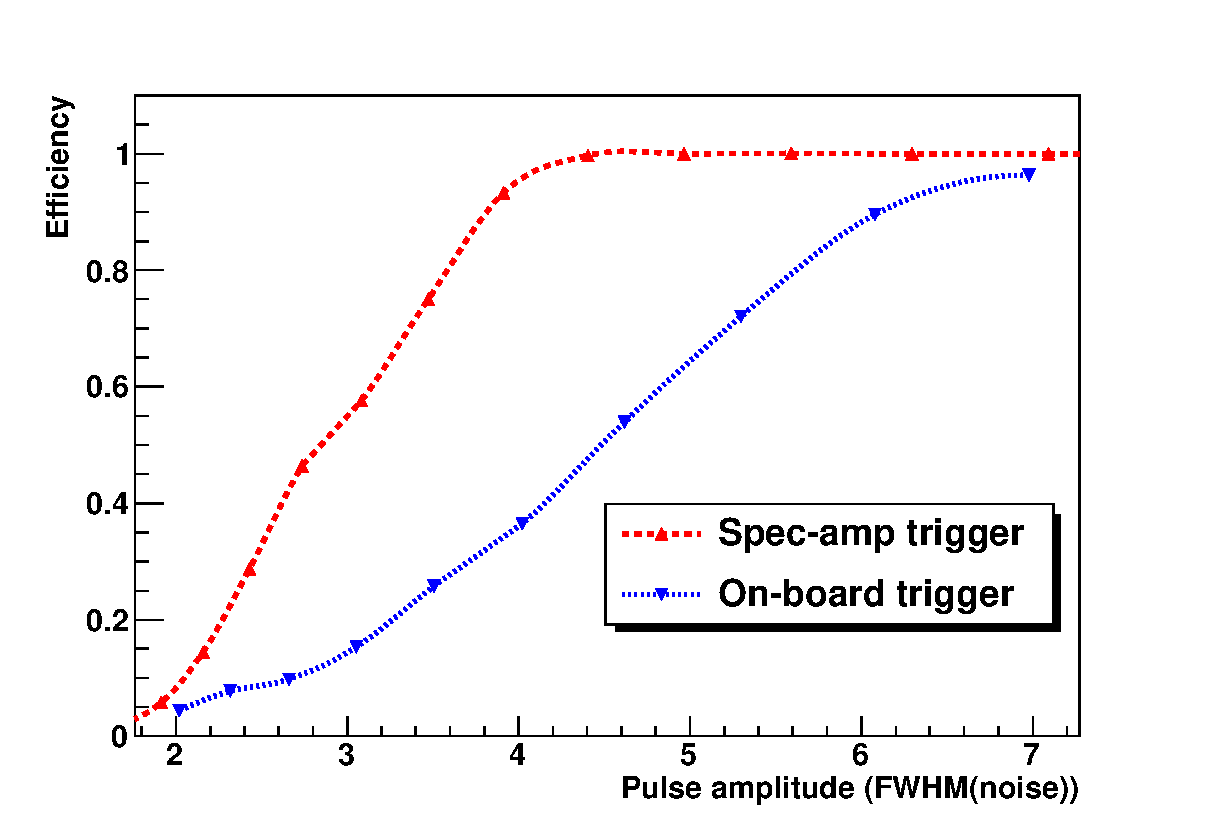
\includegraphics[width=0.9\textwidth]{EfficiencyThreshold}
				\caption[Triggering efficiency test results]
				{Triggering efficiency test results comparing the on-board LED trigger to the 
				hybrid system.  The hybrid system was found to have a factor of $\sim$2 improvement.}
				\label{fig:PPC2TriggeringEfficiencyTests}
			\end{figure}

		\subsection{Measured electronic noise}
		\label{sec:DeploymentPPC2SoudanAnalysisElectronicNoise}    
	
	The electronic noise was measured by injecting a pulse from the waveform generator and calculating the FWHM of the width of the peak.  Since this calculation was performed offline, the parameters of the trapezoidal filter (i.e. integration time and collection time) could be varied over the same data set to determine the values which would yield the best resolution.  The trace length of the waveform was limited to 10~$\mu$s and, since the rising edge of the waveform was positioned in the middle of the digitization window, the offline filter integration length was limited to less than 5~$\mu$s.  In practice, the limitation on the integration time was closer to 3.5~$\mu$s to account for variations in the position of the rising edge of the pulse with different pulse amplitudes.  Results, shown in Figure~\ref{fig:PPC2NoiseVsIntegrationTime}, indicate that the best resolution comes at the longest shaping time and also suggest that the minimum resolution could not be achieved with this setup.  The minimum value measured in this test, 225~eV, was larger than the value measured with an analog electronics system, 180~eV, but it is expected that this difference would shrink if longer integration times were available.
	
				\begin{figure}
					\centering
					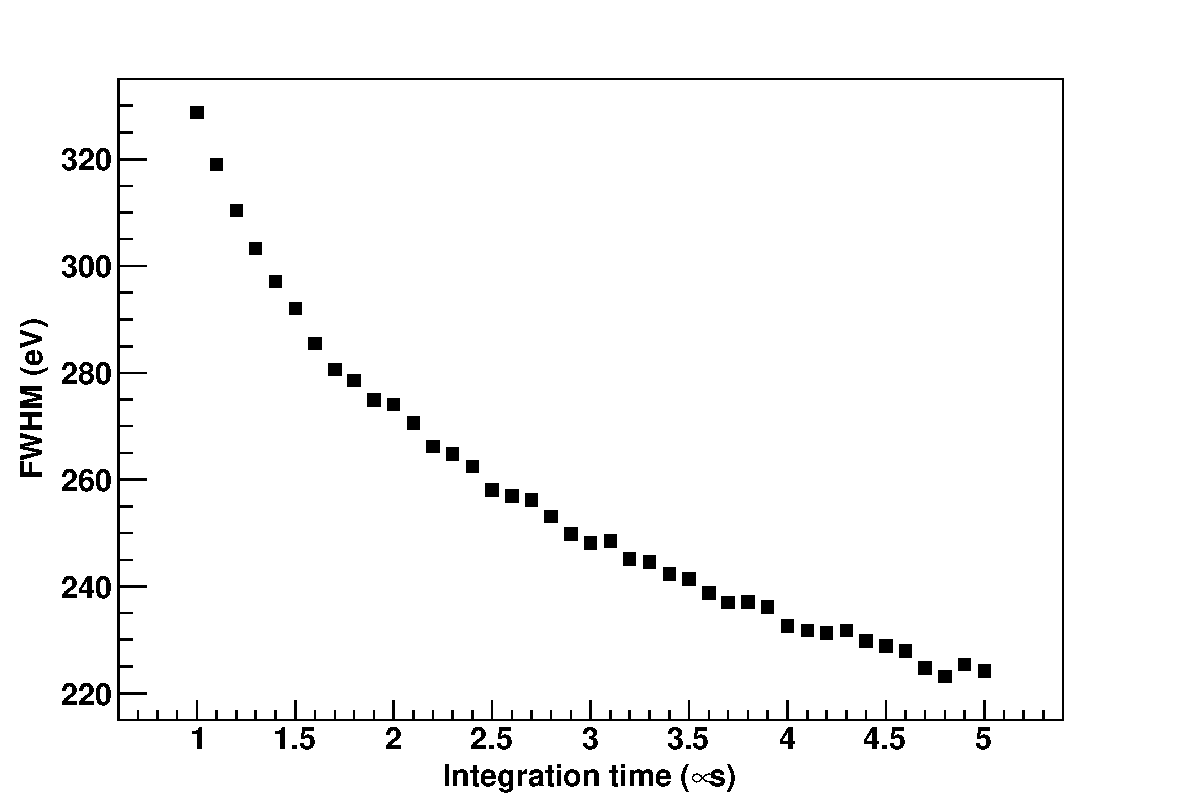
\includegraphics[width=0.9\textwidth]{filterTestTrap1d-1}
					\caption[Noise versus integration time of the trapezoidal filter]
					{Noise versus integration time of the trapezoidal filter.}
					\label{fig:PPC2NoiseVsIntegrationTime}
				\end{figure}
		
		\subsection{Conclusions}
	
	\section{Development of the Struck 3302 Digitizer}
	
		\subsection{Description of system}
	    
		\begin{table}
			\centering
			\begin{tabular}{l|c|c}
			\end{tabular}
			\caption[Differences between the Gretina Digitizer and the Struck Digitizer]
			{Differences between the Gretina Digitizer and the Struck Digitizer.}
			\label{tab:BeGeSIS3302GretinaDifferences}
		\end{table}	
	      
		\subsection{Analysis and Results}
		\label{sec:DeploymentBeGeSoudanAnalysis}
		% Description of analysis techniques used and results.  The ordering of this section could be modified.
		
			\subsubsection{Calibration}
			\label{sec:DeploymentBeGeSoudanAnalysisCalibration}    
			
				\begin{figure}
					\centering
					%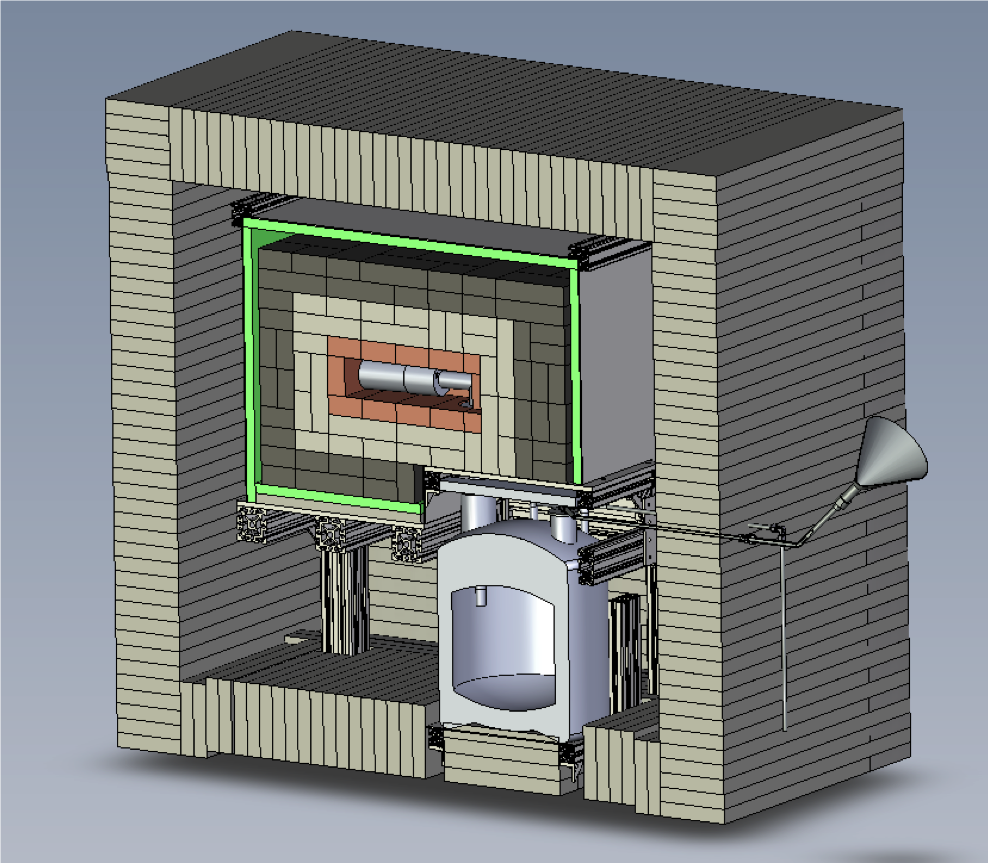
\includegraphics[width=0.9\textwidth]{PPC2DesignSchematicAll}
					\caption[Calibration of the channels]{Calibration of the channels.}
					\label{fig:BeGeCalibration}
				\end{figure}
		    
		    	\subsubsection{Trigger Efficiency}
			\label{sec:DeploymentBeGeSoudanAnalysisTriggerEfficiency}    
			
				\begin{figure}
					\centering
					%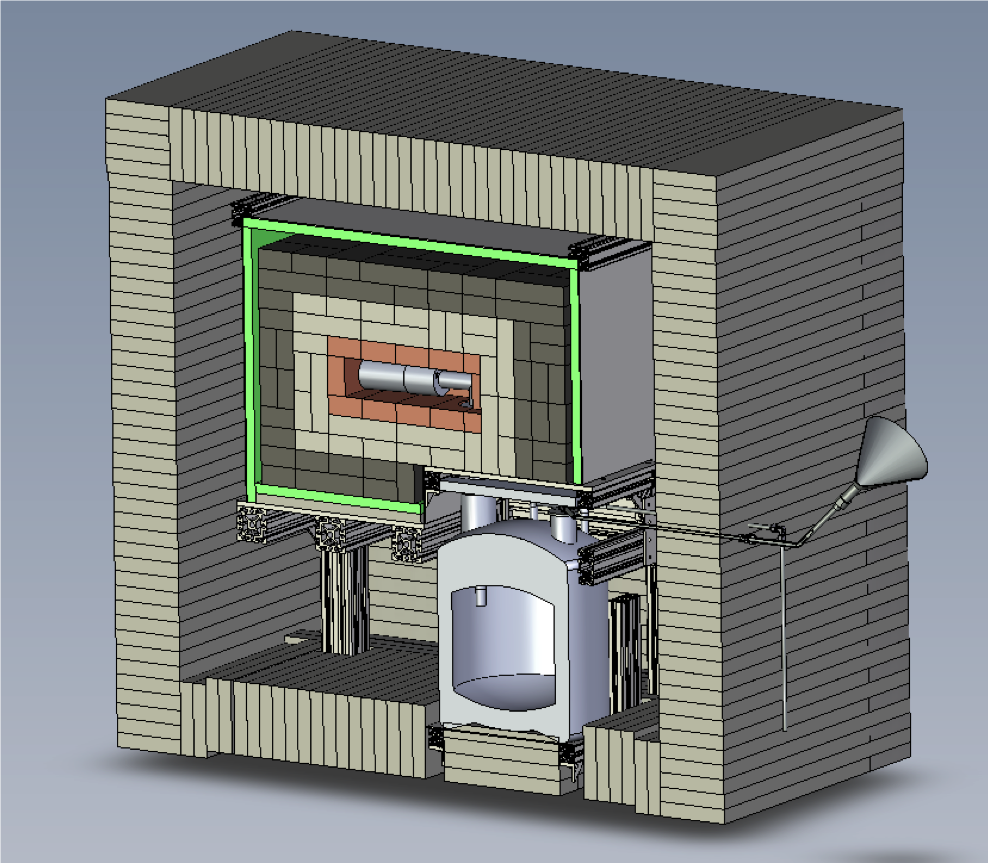
\includegraphics[width=0.9\textwidth]{PPC2DesignSchematicAll}
					\caption[Struck card triggering efficiency tests]{Triggering efficiency tests.}
					\label{fig:BeGeTriggeringEfficiencyTestsVsTime}
				\end{figure}
			
		    	\subsubsection{Noise measurement}
			\label{sec:DeploymentBeGeSoudanAnalysisNoiseMeasurment}    
			
				\begin{figure}
					\centering
					%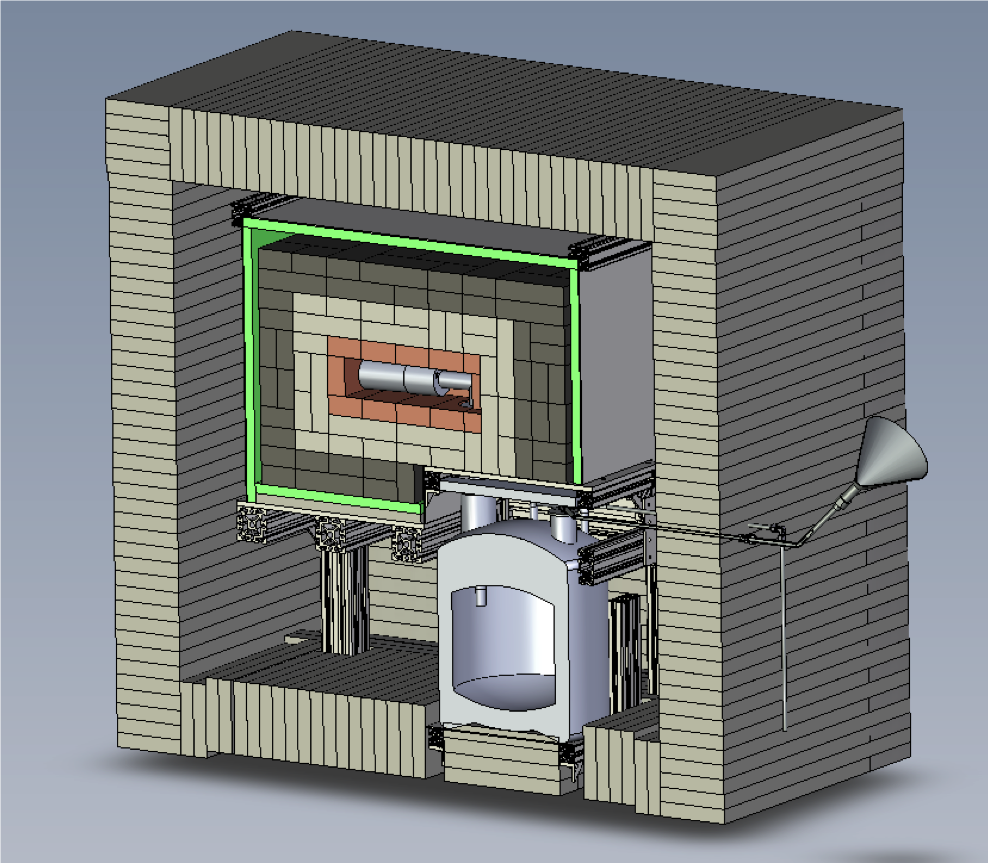
\includegraphics[width=0.9\textwidth]{PPC2DesignSchematicAll}
					\caption[Struck noise measurement versus integration time]
					{Noise measurement versus integration time.}
					\label{fig:BeGeTriggeringNoiseMeasurment}
				\end{figure}
						
		    	\subsubsection{Energy spectra}
			\label{sec:DeploymentBeGeSoudanAnalysisEnergySpectra}    		
	
				\begin{figure}
					\centering
					%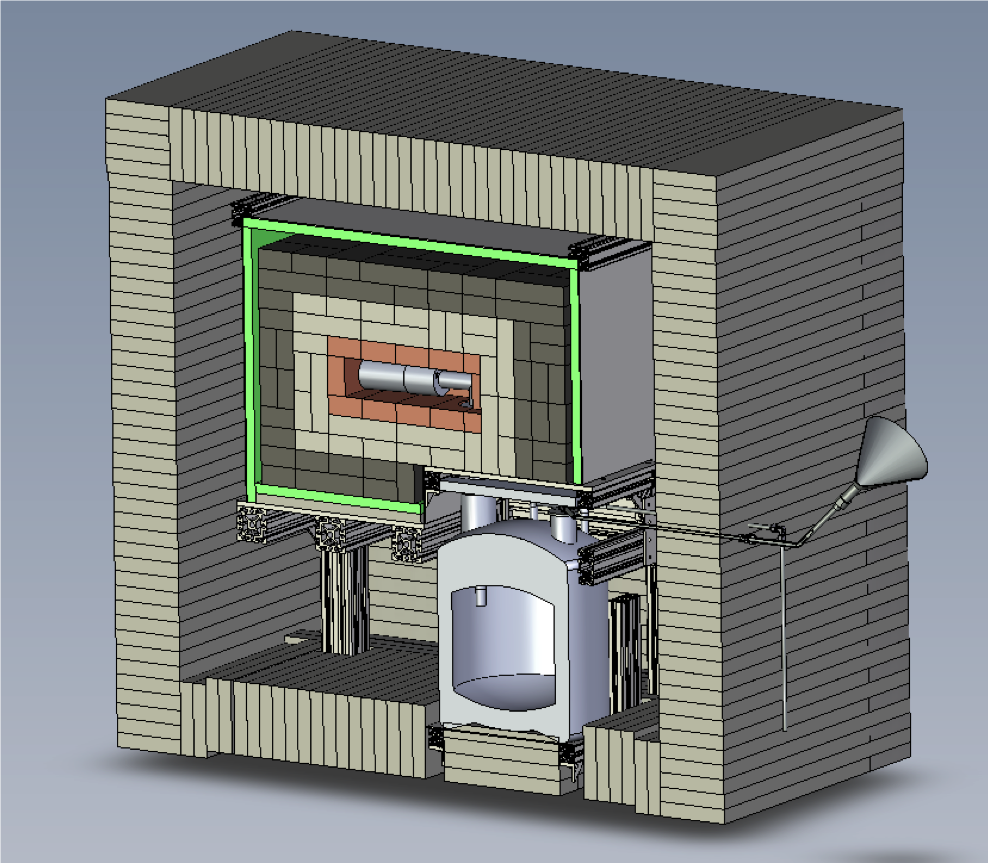
\includegraphics[width=0.9\textwidth]{PPC2DesignSchematicAll}
					\caption[Struck energy spectrum from high- and low-gain channels]
					{Energy spectrum from high- and low-gain channels.}
					\label{fig:BeGeEnergySpectrum}
				\end{figure}      
				
		\subsection{Conclusions}	
		    




 
\clearpage

% ========== Chapter 3
 

\chapter{Deployment of a Digital DAQ for a \ppc~detector at the Soudan Underground Laboratory}
\label{chap:DeploymentPPC2Soudan}
	\section{Introduction}
	\label{sec:DeploymentPPC2SoudanIntro}
			
		A \ppc~detector (henceforth referred to as \ppc2) was procured by Pacific Northwest National Laboratory in January 2008 to be used in studies aimed at more clearly understanding the detector technology~\cite{Orr2007}.  Initial tests took place in the laboratory, focusing on basic operation and pulse-shape analysis techniques relevant for background reduction in the $\nonubb$ region-of-interest and for dark matter searches~\cite{Orr2008}.  In November 2008, \ppc2 was deployed underground at Soudan Underground Laboratory at a depth of 2100~m.w.e.  The goals of this deployment were two-fold: (1) demonstrate the reliability and operation of a scaled-down \MJ-like digital DAQ system in an underground environment, and (2) investigate the possibility of obtaining Dark Matter exclusion data.  The latter goal was uncertain due to the lack of knowledge of the intrinsic backgrounds of the detector and its cryostat.  
		%The development of the DAQ system used in this deployment is outlined in Chapter~\ref{chap:DAQDevel}
		
		Underground, the detector was placed inside 8~inches of Pb with a 2-inch inner shield composed of OFHC Cu.  This shield was surrounded by a sealed radon-exclusion box over-pressurized with nitrogen gas from LN boil-off to limit the introduction of Rn gas.  Borated-polyethylene planks were built up surrounding the outer lead for moderation of neutrons generated by interactions of cosmic-ray muons in the rock walls.  An engineering drawing of the shield can be seen %in Figure~\ref{fig:PPC2OnlyShield} and 
with all components in Figure~\ref{fig:PPC2Shield}.  Relevant characteristics of the crystal are given in Table~\ref{tab:PPC2Characteristics}.
	
			%\begin{figure}
			%	\centering
			%	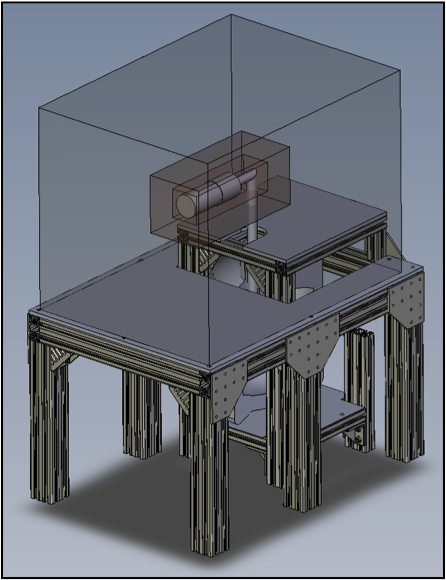
\includegraphics[width=0.6\textwidth]{PPC2DesignSchematicShield}
			%	\caption[Engineering drawing of \ppc2 deployment]
			%	{Engineering drawing of the setup including inner and outer Cu and Pb shields which rests upon the frame.
			%	Graphic courtesy of J.~Orrell and E.~Fuller.}
			%	\label{fig:PPC2OnlyShield}
			%\end{figure}
	
			\begin{figure}
				\centering
				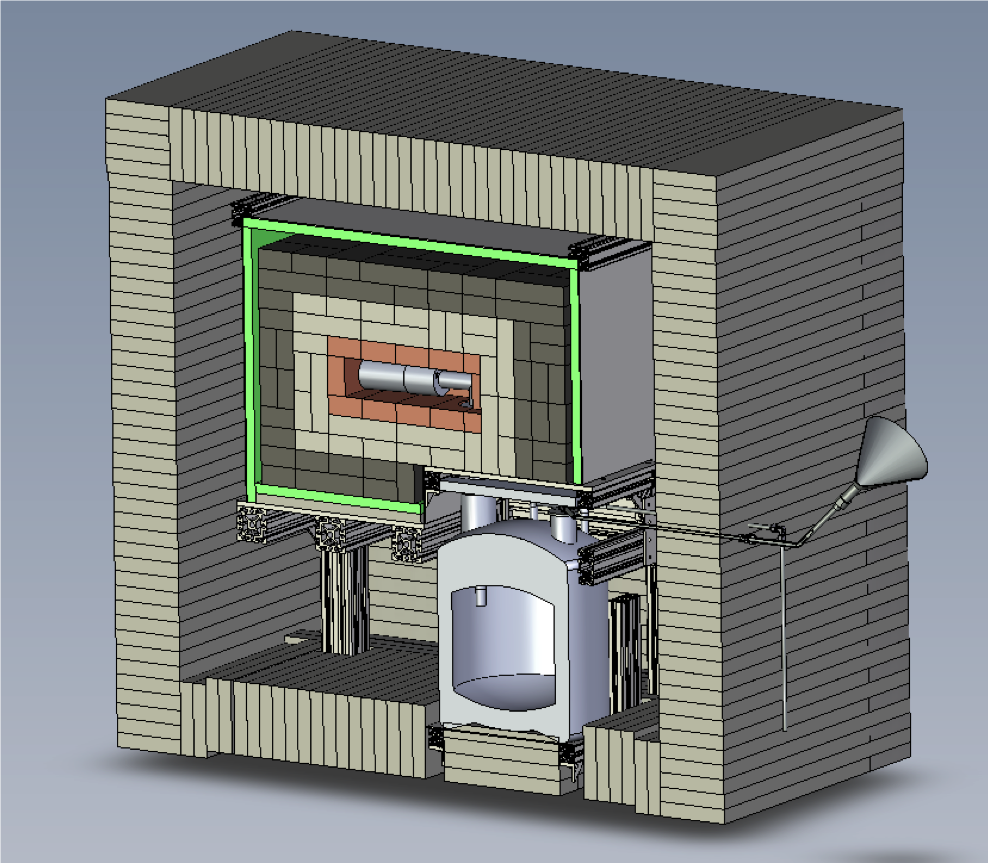
\includegraphics[width=0.9\textwidth]{PPC2DesignSchematicAll}
				\caption[Engineering drawing of \ppc2 deployment, detailing outer components]
				{Engineering drawing of the setup including inner and outer Cu and Pb shields, Rn exclusion box, 
				and outer neutron moderator.  The two colors for the lead outside of the copper inner
				shield were an internal designation specifying `cleaner' lead (with less oxidization, better cosmetic appearance,
				 etc.) to be used closest to the inner shield.  Graphic courtesy of J.~Orrell and E.~Fuller.}
				\label{fig:PPC2Shield}
			\end{figure}
	
			\begin{table}
				\centering
				\begin{tabular}{l r}
					\toprule
					Property & Value \\
					\midrule
					Manufacturer & Canberra \\
					Mass & 528 g \\
					Outer diameter & 50.1 mm \\
					Length & 50.3 mm \\
					Useful volume & 89.4 cm$^{3}$\\
					Dead layer & 0.5 mm \\
					% FixME include contact diameter
					\bottomrule
				\end{tabular}
				\caption[\ppc2 detector characteristics]
				{\ppc2 detector characteristics.  }
				\label{tab:PPC2Characteristics}
			\end{table}
	
	\section{Description of DAQ system}
	\label{sec:DeploymentPPC2SoudanDAQSystem}
	
	The DAQ system was designed as a single-channel prototype for the \MJ~\minmod.  Additionally, a significant amount of effort was put in to ensure that the setup was remotely configurable to enable the modification of experimental parameters from experimenters at the University of Washington and PNNL.  Signals from the detector were read out using a Gretina Mark IV digitizer designed by the GRETA collaboration~\cite{Anderson:2009p1293}.  This VME64x-based ADC digitized 10 independent channels at 100~Ms/s with a resolution of 14 bits.  The card was read out on the VME backplane using a Concurrent Technologies VX 407/042 single-board computer controlled via gigabit ethernet by the ORCA DAQ and slow controls software~\cite{ORCA} running on an Apple Mac Mini computer.  For more details regarding the ORCA DAQ software and the development of its components relevant to this hardware configuration, please see Appendix~\ref{app:ORCASoftwareChapter}.  Also, additional details regarding the development and investigation of this DAQ system are given in Chapter~\ref{chap:DAQDevel}. The high voltage on \ppc2 was controlled via a Canberra LYNX system which allowed for remote powering on and off of the detector bias.  The Liquid Nitrogen (LN) dewar was filled manually by the laboratory staff so no explicit tag was set in the data stream during these fills.  Techniques to identify and cut out these events are discussed in Section~\ref{sec:DeploymentPPC2SoudanAnalysisCuts}.
	    
	As with many low-noise designs, the \ppc2 preamp employed a pulse-reset circuit to avoid the Johnson noise associated with a feedback resistor.  The preamp had 3~outputs: 2~signal outputs and 1~inhibit output which would fire when the reset circuitry of the preamp was active.  Additionally, there was a test input for pulser signals used in electronic testing.  The 2~signal outputs were AC-coupled to remove their DC components using independent capacitors of $\sim500$~nF to yield a roughly 50~$\mu$s decay time of the preamp pulses.  One of these channels was input directly into the digitizer; the other was routed through a Phillips Scientific 777 fast amplifier (DC$\to$200~MHz bandwidth) with roughly $10\times$ gain to obtain better resolution near threshold from $0.5\to80$~keV.  The signal was split after the 777, with one output being input into a digitizer channel in the Gretina card and the other routed through a conventional spectroscopy amplifier (Ortec 667) to generate the trigger for the high-gain channel.  Figure~\ref{fig:PPC2DAQSetup} provides a simplified visualization of the DAQ setup including signal paths.  See Section~\ref{sec:DeploymentPPC2SoudanTriggerDesign} for more details regarding the high-gain trigger and its development.  The inhibit output was sent directly into the Gretina digitizer card to record the timing information of the reset circuitry.
	
	The test input of the preamp was used for pulser signals to measure the efficiency of the trigger.  The pulser used was an Agilent 33220A waveform generator controlled via ethernet by ORCA running on the Mac mini.  The pulser output passed through 2~computer-controlled attenuators (HP 8494/5G, 0$\to$4~GHz bandwidth) providing up to 71~dB of attenuation in increments of 1~dB.  These attenuators were actuated using a constructed driver box controlled with an InterPak 408 digital I/O card on the VME bus.  For more details on the pulser test setup, see Section~\ref{sec:DeploymentPPC2SoudanTriggerDesign}.  A synchronization pulse from the Agilent was input into a digitizer channel for timing information.  The pulser was also used during counting runs, inputting a signal of low amplitude, $\sim$2.5~keV, into the DAQ system at low rate $\sim1$~Hz, with the purpose of measuring any deviations in the electronics over time.
		     
	A summary of the input channels on the Gretina card including the type of data saved for each is given in Table~\ref{tab:PPC2DAQChannelInfo}.  
%A schematic of the DAQ setup is shown in Figure~\ref{fig:PPC2DAQSetup}.  
The DAQ system was fully deployed underground at the beginning of April 2009.
		 
			\begin{table}
				\centering
				\begin{tabular}{l c c}
					\toprule`
					Type & Channel &  Info \\
					\midrule
					Reset inhibit & 9 & Only timing \\
					Low-gain signal & 8 & 10~$\mu$s trace (1022	 samples) \\
					Pulser sync & 7 & Only timing \\
					% FixME Muon veto hasn't been noted yet in the chapter.
					Muon veto & 2 & Only timing, unused in analysis \\			
					High-gain trigger & 1 & Only timing \\
					High-gain signal & 0 & 10~$\mu$s trace (1022 samples) \\				
					\bottomrule
				\end{tabular}
				\caption[Channel summary for the Gretina digitizer card]
				{Channel summary for the Gretina digitizer card.  }
				\label{tab:PPC2DAQChannelInfo}
			\end{table}	     
	
	
			\begin{sidewaysfigure}
				\centering
				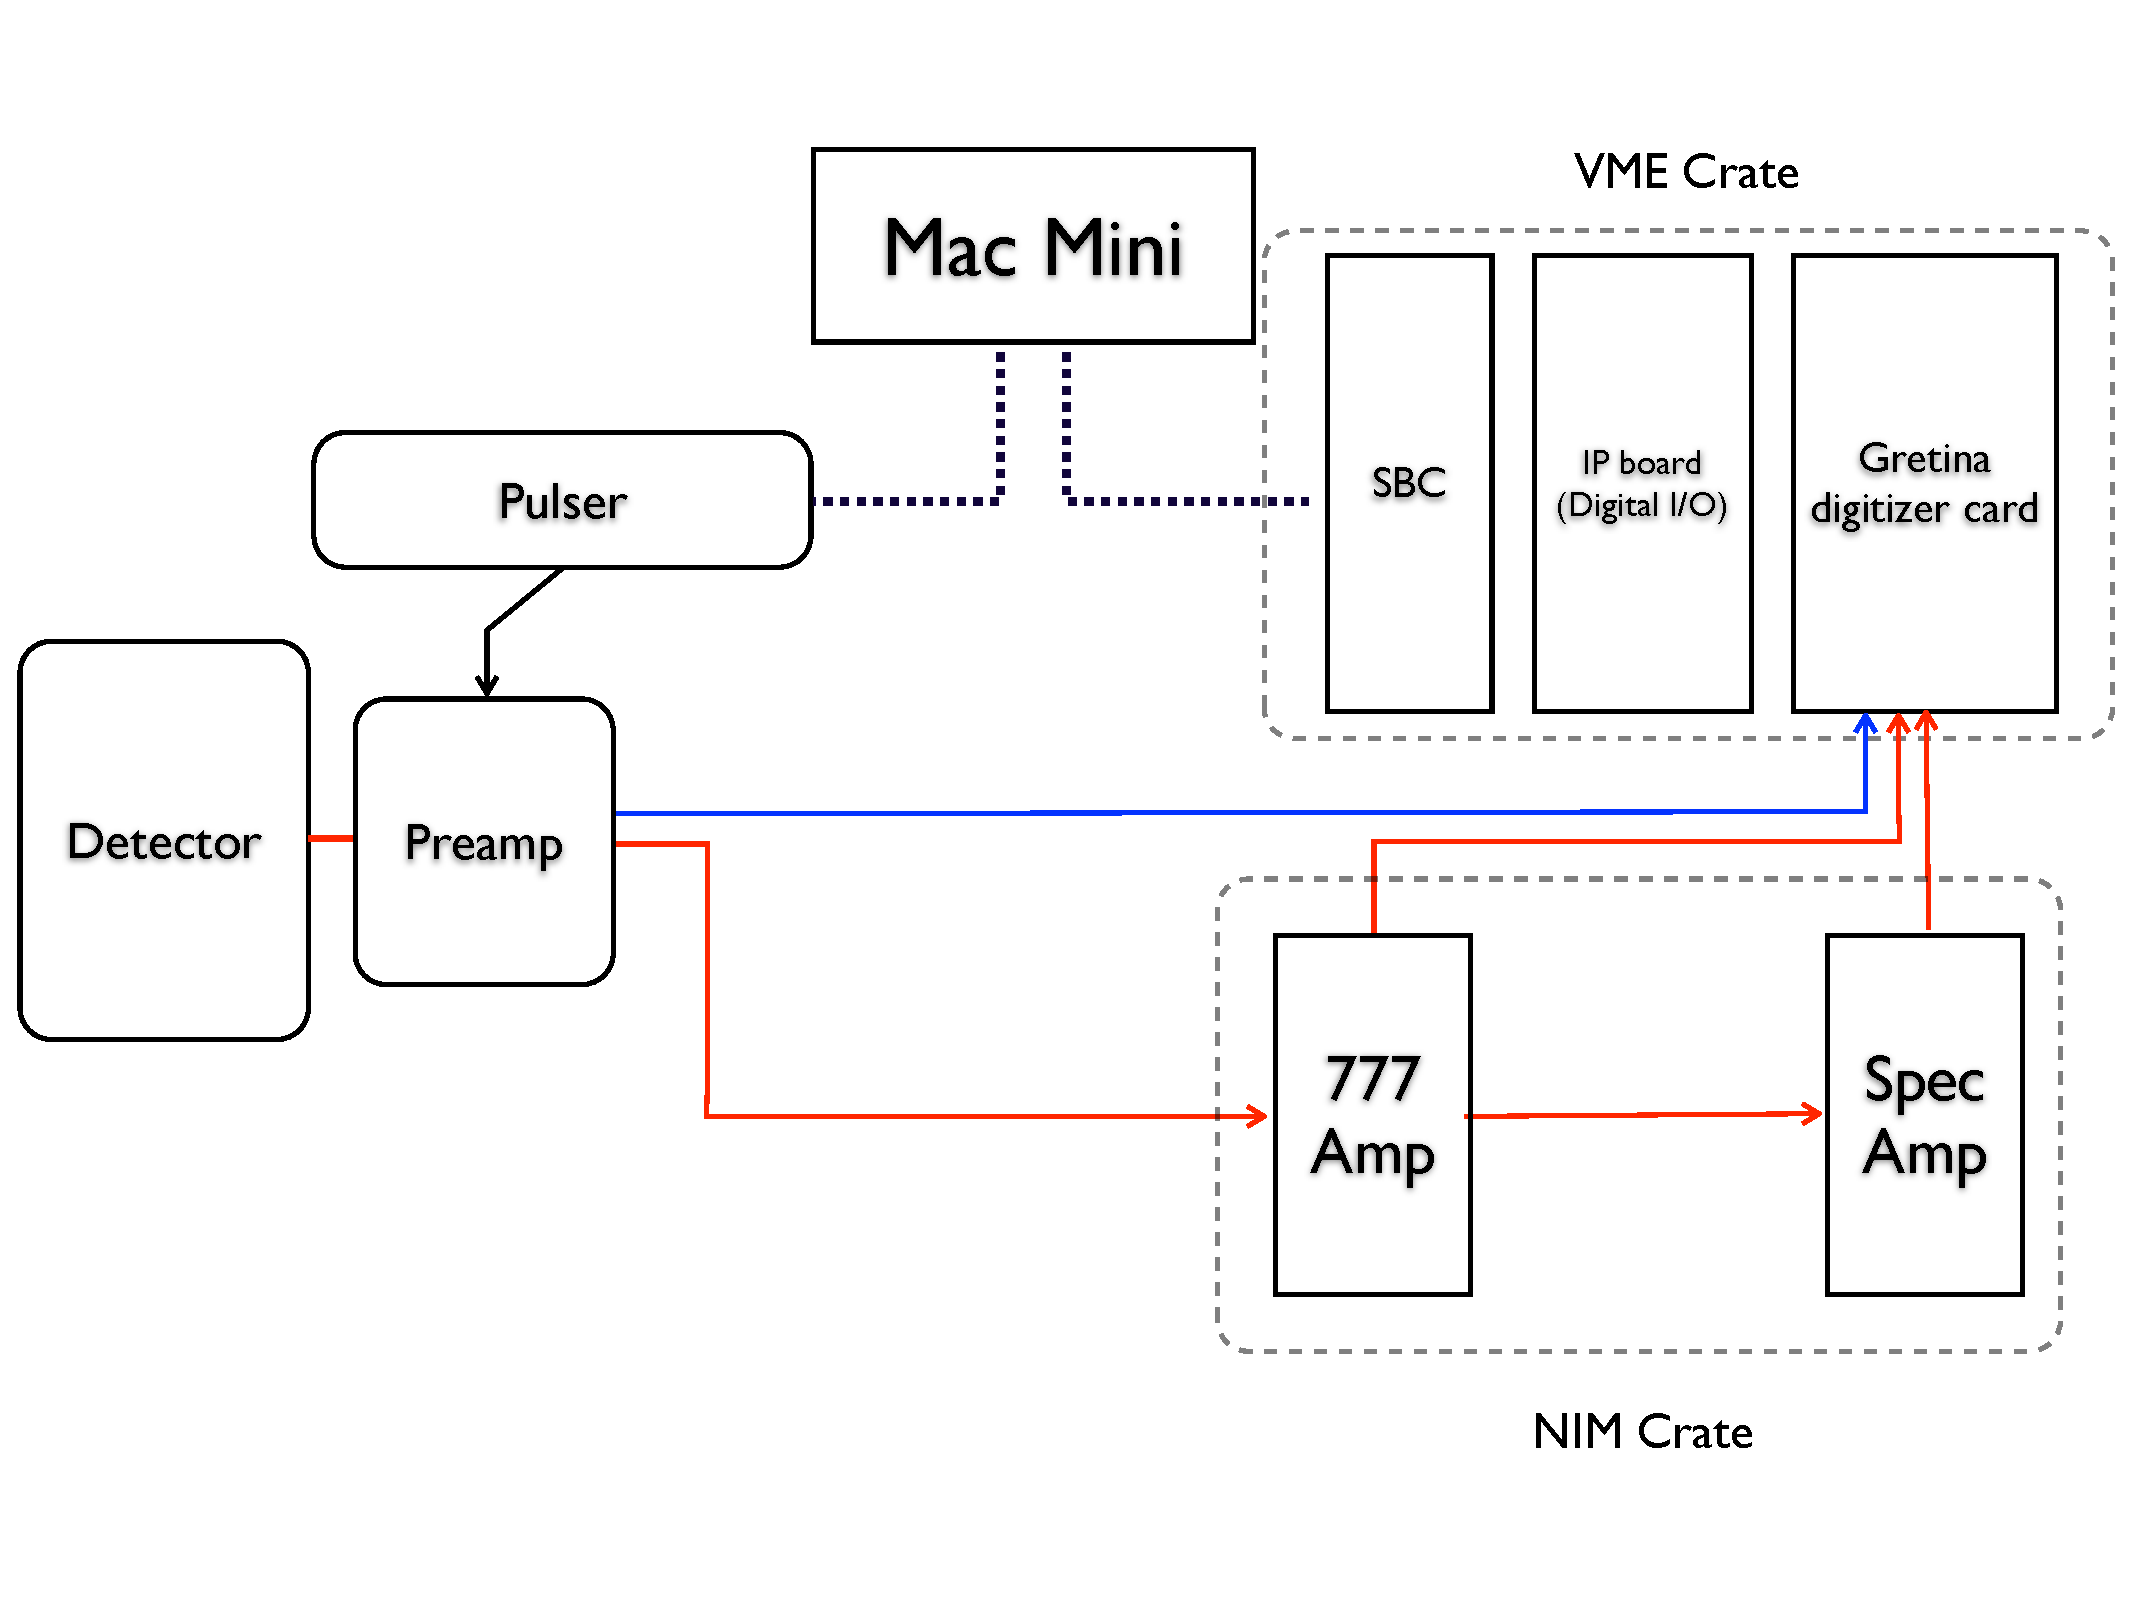
\includegraphics[width=0.95\textwidth]{PPC2DAQSchematic}
				\caption[Simplified schematic of DAQ setup] 
				{Simplified schematic of DAQ setup.  Lines with arrows denote signal flow.}
				\label{fig:PPC2DAQSetup}
			\end{sidewaysfigure}
		     			
	\section{Analysis and Results}
	\label{sec:DeploymentPPC2SoudanAnalysis}
	
	After a few months of commissioning and calibration tests, counting runs were begun on 3 May 2009.  Runs were cycled every hour, and data were automatically synchronized with a server at the University of Washington.  On 10 June 2009, automatic trigger efficiency tests were begun in between runs to monitor the stability of the trigger over time.  Counting runs ended on 24 July 2009, yielding a total live-time of 70.4 days.  A CouchDB database~\cite{CouchDB} was used to store both metadata (e.g.~timing, configuration, file names, etc.) as well as analysis parameters (e.g.~average baseline, trigger efficiency, measured electronic noise) from each run.  This database was also used to facilitate the analysis chain described in the following section.    

		\subsection{Data processing}
		\label{sec:DeploymentPPC2DataProcessing}	
	
	All data were handled in a tiered reduction scheme.  The analysis process was automated and made significant use of the ROOT analysis framework~\cite{Bru97} as well as waveform analysis tools (MGDO, see Appendix~\ref{app:MGDO} for more information) developed for the \MJ~experiment.  An outline of the tiered data-flow process is given:
		\begin{description}\itemsep2pt
			\item[Tier 0:]  Raw binary data -- from the ORCA DAQ system
			\item[Tier 1:]  ROOTified data -- raw data converted to MGDO objects and stored in ROOT TFiles
			\item[Tier 2:]  Waveform processed data -- extraction of waveform characteristics using MGDO Transforms
			\item[Tier 3:]  Reduced data and split into sub-components according to different channels
		\end{description}	
		
	This process was tracked using a CouchDB database.  The Tier~$0\to1$ conversion process took the raw binary data and converted it into MGDO \cpp~objects which could then be serialized to disk in ROOT TFiles.  The Tier~$1\to2$ processing calculated several parameters from the waveform data, including baseline, extrema (maximum and minimum), and rise-time and determined the amplitude of the waveform using a trapezoidal filter\footnote{The Gretina digitizer included an on-board trapezoidal filter, but it was chosen to use an offline filter for greater flexibility.}~\cite{Jor94}.  More information regarding the baseline and rise-time calculations are given in Sections~\ref{sec:DeploymentPPC2SoudanAnalysisCuts} and~\ref{sec:DeploymentPPC2SoudanAnalysisRisetime}.  Additionally, at this stage coincidences between events in different channels were calculated using the timing information from the digitizer card, defining events within $1~\mu$s of each other as concurrent.   Finally, the Tier~$2\to3$ processing reduced the data size, removing noise events (i.e.~events well below energy threshold) and splitting the two signal channels 0 and 8 into separate file groups.  The Tier~3 files were used directly in analysis and made available to others in the \MJ~collaboration through a cloud-based file system (Dropbox\footnote{See the Dropbox website: \url{https://www.dropbox.com} for more information.}).
	
		\subsection{Initial calibration}
		\label{sec:DeploymentPPC2SoudanAnalysisCalibration}    
			
	The system was initially calibrated with a $^{133}$Ba source using peaks detailed in Table~\ref{tab:Ba133Peaks}.  The high- and low-gain channels were calibrated independently and spectra for each channel are shown in Figure~\ref{fig:PPC2Calibration}.  The two channels exhibited an energy range up to $\sim100$~keV and $\sim 2.6$~MeV, respectively, though the range of the low-gain channel is discussed in more detail in Section~\ref{sec:DeploymentPPC2SoudanAnalysisEnergySpectra} .  These initial calibrations were used for commissioning tests such as trigger efficiency and electronic noise measurements and were later refined using prominent peaks from backgrounds e.g.~in the U and Th chains, $^{40}$K, and x-ray lines from \gersixeight~and \znsixfive~electron capture decays (see Section~\ref{sec:DeploymentPPC2SoudanAnalysisEnergySpectra}).  During the counting runs, regular calibration runs were not made; instead we monitored the behavior of the detector using an injected pulser.  

				\begin{table}
					\centering
					\begin{tabular}{l r}
						\toprule
						Energy (keV) & Intensity \\
						\midrule
						    53.16 	 &     2.2 \% \\ 
						    79.61 	 &     2.62 \% \\
						    80.997 	 &    34.1 \%\\
						   160.61 	 &     0.65 \%\\
						   223.24 	 &   0.45 \% \\
						   276.4 	 &     7.16 \% \\
						   302.85 	 &   18.33 \% \\
						   356.01 	 &    62.05 \% \\
						   383.85 	  &    8.94 \% \\
						\bottomrule
					\end{tabular}
					\caption[Selected gamma lines used for calibration in the $^{133}$Ba spectrum]
					{Selected gamma lines used for calibration in the $^{133}$Ba spectrum, 
					data adapted from~\cite{Rab1995491}.}
					\label{tab:Ba133Peaks}
				\end{table}	
						
				\begin{figure}
					\centering
					\subfigure[High-gain channel]{
						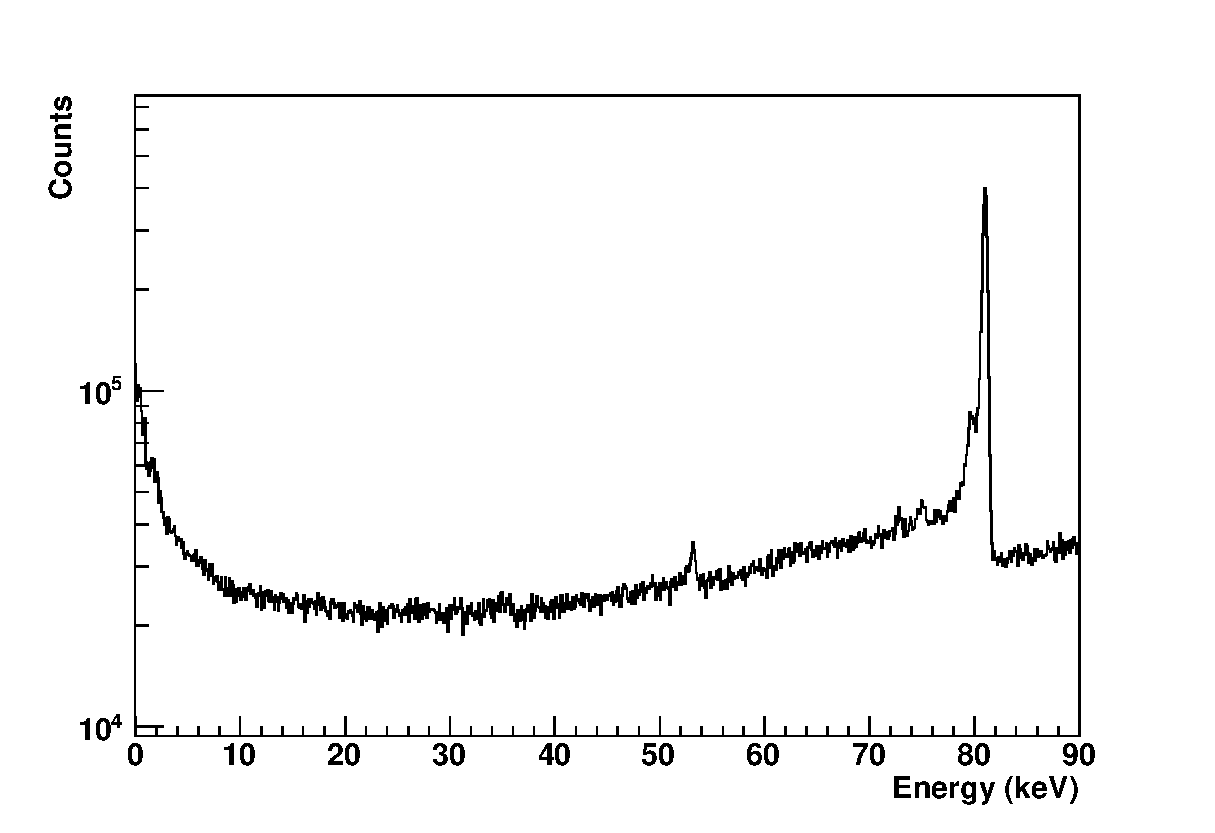
\includegraphics[width=0.9\textwidth]{LowEnergyCal}
						\label{fig:PPC2CalLow}
					}
					\subfigure[Low-gain channel]{
						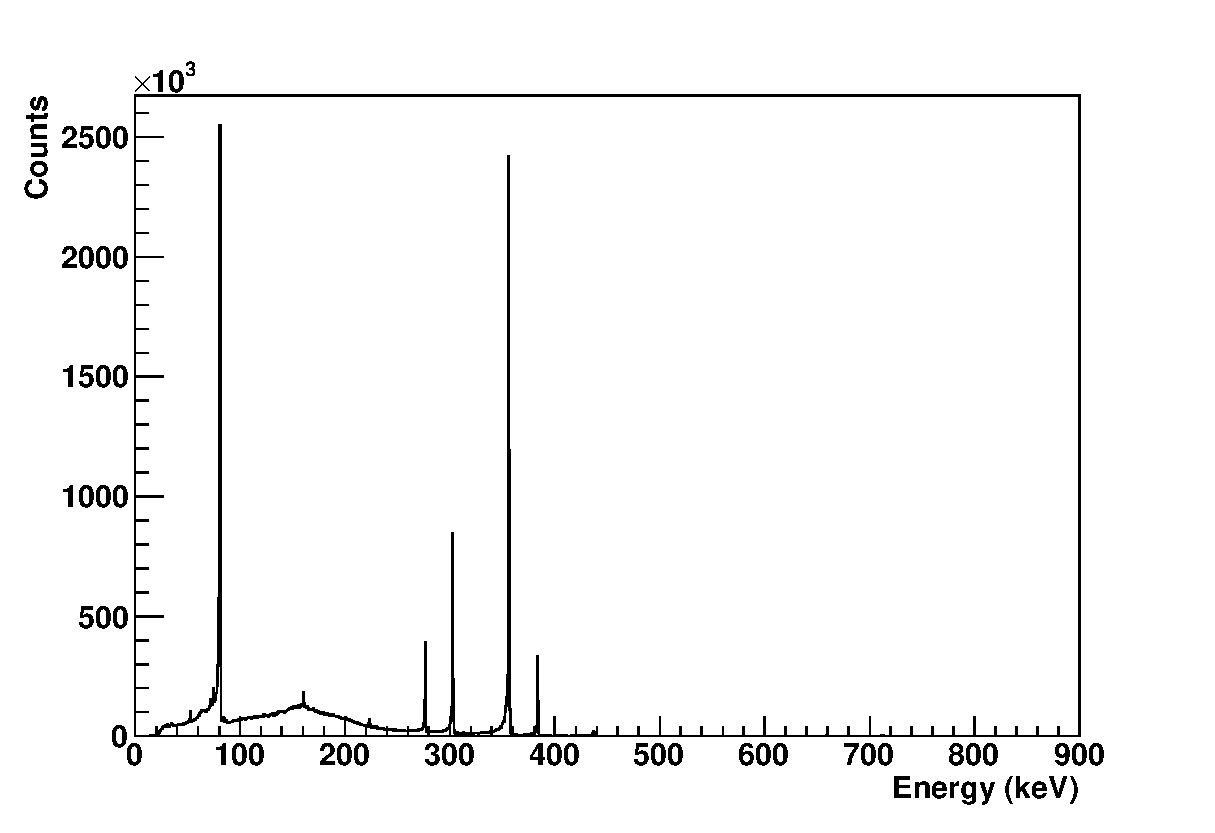
\includegraphics[width=0.9\textwidth]{HighEnergyCal}
						\label{fig:PPC2CalHigh}
					}
					\caption[Calibration of the high- and low-gain channels]
					{Calibration of the high- and low-gain channels.}
					\label{fig:PPC2Calibration}
				\end{figure}

		\subsection{Detector parameters vs.~time}	
		\label{sec:PPC2DetParsVsTime}
		
	Several parameters of the system were tracked over time, including the trigger efficiency and the electronic noise of the system.  The former was tested by performing efficiency tests every hour in between run cycles; the latter by looking at the recorded data of the input pulser pulses (1~Hz) versus time.  Several other parameters, including the baseline of the waveforms and the number of events in a certain energy ranges, were tracked as well: these results are presented in Section~\ref{sec:DeploymentPPC2SoudanAnalysisCuts}.  In addition to these specific parameters being tracked, the rates of each channel were tracked.  While tracking these rates, it was determined that the reset rate of the preamp increased towards the end of an LN fill cycle.  Higher values of inhibit rate (lower baseline values) occurred as LN in the dewar boiled off, with sharp returns when the dewar was refilled.  The interpretation of this was that as the level of LN in the dewar fell, the temperature of the front-end detector electronics (and possibly the crystal) would increase which would increase the detector leakage current.  An increase in leakage current would cause the preamp to reset more often to clear the charge more quickly accumulating on the feedback capacitor.  It was not determined precisely what caused this temperature sensitivity; however, it was likely due to insufficient thermal coupling between the detector and the liquid nitrogen.  During installation of the detector within the Pb shield, an extension had to be added to the dewar end of the cold finger.  It is possible that this extension didn't properly thermally couple to the cold finger and thus didn't cool the detector and/or the internal electronics as effectively.  The change of the reset rate over time had implications for other parameters as discussed in the following sections.  A summary of comparisons between detector parameters is shown in Figure~\ref{fig:PPC2AllPlotCompare}.  In this figure, LN fills occurred around runs~1590, 1665, and 1750.  The average values of the parameters in the following sections is given in Table~\ref{tab:PPC2AvgPars}.
	
% FixME, move comparison plot around?

		    	\subsubsection{Pulser data}
			\label{sec:DeploymentPPC2SoudanAnalysisPulserData}    

	Pulses from the Agilent waveform generator were input into the test input at a rate of 1~Hz and at low energy: $\sim2.5$~keV.  These events underwent analysis equivalent to every other waveform and were selected by finding all waveforms which arrived in coincidence with the pulser synchronization signal.  Each hour-long run yielded a data set of $\sim3600$ events; the calculated amplitudes (energies) of these events were histogrammed and fit to a gaussian to extract the mean, $\mu$, and the sigma, $\sigma$, of the pulser signal for each run.  Results of these fits are plotted versus run number in Figure~\ref{fig:PPC2AllPlotCompare}.  It is clear that the width of the noise ($\sigma$) did not significantly alter for reset rates below 15~Hz.  However, the mean ($\mu$) of the pulser demonstrated three clear transition regions an example of which have been labeled `I', `II', and `III' in Figure~\ref{fig:PPC2AllPlotCompare}: from reset rates 3$\to$7~Hz (region I labeled in the plot), the mean increased, transitioned to lower values for reset rates 7$\to$11~HZ (region II), and then returned for rates above 11~Hz (region III).  The absolute cause of this behavior was not determined, but it is possibly due to a modification of operating parameters of the front-end crystal electronics (e.g.~the FET) by the increasing leakage current.  

			%%%%\begin{figure}
			%%%%	\centering
			%%%%	\subfigure[Pulser sigma, $\sigma$, vs.~time.]{
			%%%%		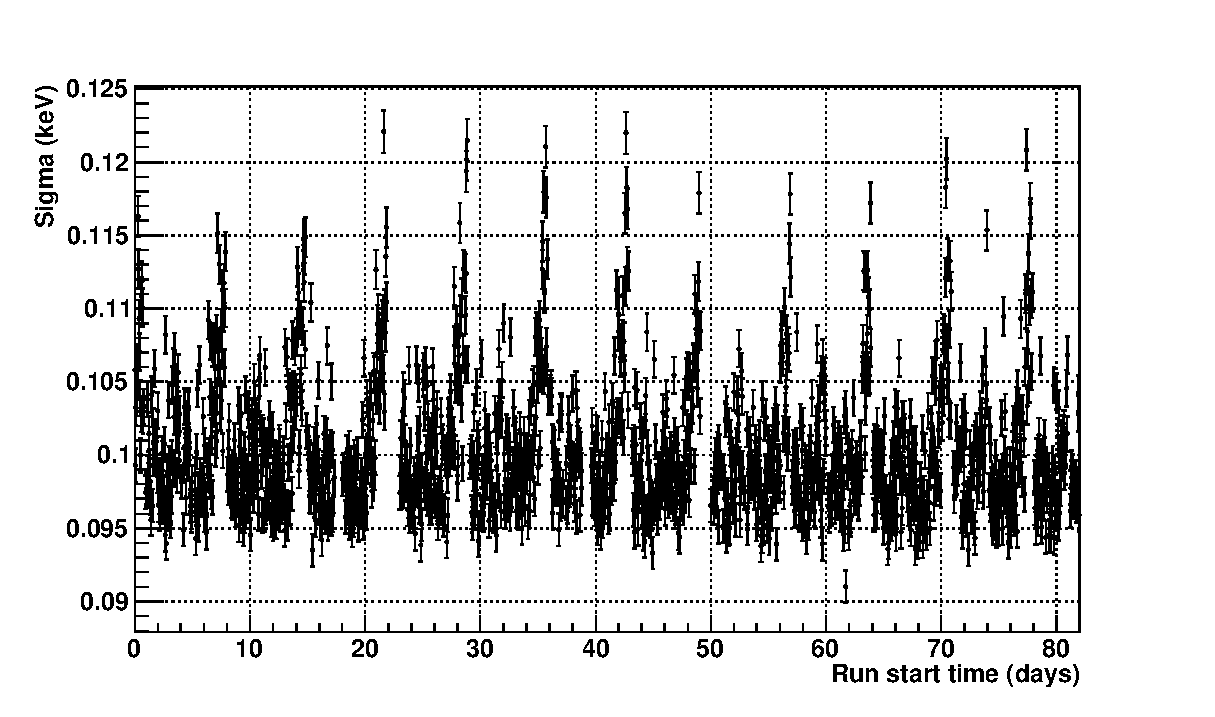
\includegraphics[width=0.45\textwidth]{PulserSigmaVsTime}
			%%%%	}
			%%%%	\subfigure[Pulser mean, $\mu$, vs.~time.]{
			%%%%		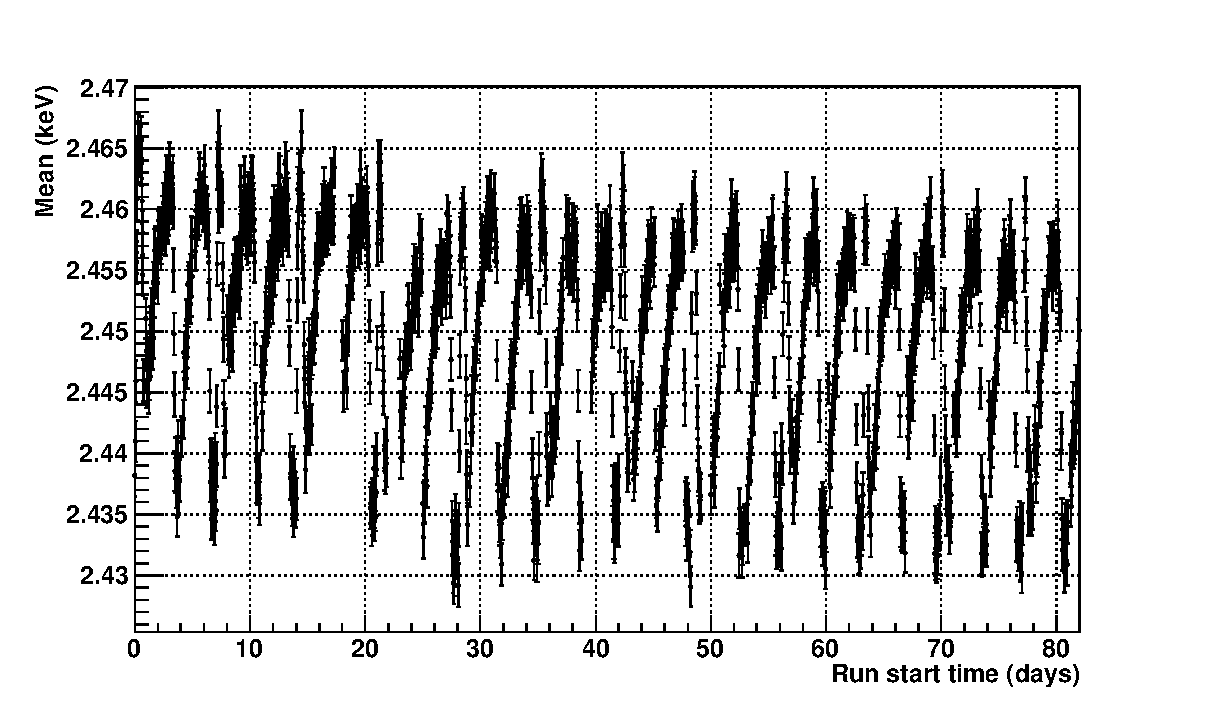
\includegraphics[width=0.45\textwidth]{PulserMeanVsTime}
			%%%%	}						
			%%%%	\caption{Measured $\mu$ and $\sigma$ of pulser versus run start time.}
			%%%%	\label{fig:PPC2PulserVsTime}
			%%%%\end{figure}



		    	\subsubsection{Trigger Efficiency}
			\label{sec:DeploymentPPC2SoudanAnalysisTriggerEfficiency}    
			
	Trigger efficiency was measured as described in Section~\ref{sec:DeploymentPPC2SoudanTriggerDesign}.  Initial tests were performed during the commissioning period (i.e.~before counting runs began) and automatic tests were run after every hour-long cycle beginning 38~days into the counting run period.  The goal of these tests was to investigate how the trigger threshold behaved over time, tracking any changes that might occur due to shifts in environmental conditions or because of other unforeseen phenomena.  To parameterize the efficiency, the data were fit to an error function, $f_{eff}(E)$, in the form:

				\begin{equation}
					f_{eff}(E) = \frac{1}{2} - \frac{1}{2} \operatorname{erf} \left( s ( E-\rho ) \right)
					\label{eqn:TriggerEfficiency}
				\end{equation}
				
with energy, $E$, in keV; scaling parameter, $s$, in keV$^{-1}$; and offset, $\rho$, in keV.  An example of a fit to this data is given in Figure~\ref{fig:PPC2TriggeringEfficiencyExample}.  Some results of the trigger tests over time are given in Figure~\ref{fig:PPC2AllPlotCompare}, comparing them to other detector parameters.  The offset parameter, $\rho$, was largely stable but increased before the transition from I$\to$II and again during region III.  $\rho$ returned to a lower value during region II.  The scaling, $s$, was largely insensitive to any change in reset rate, though exhibited slight deviations low in transitions between regions I and II.  

				\begin{figure}
					\centering
					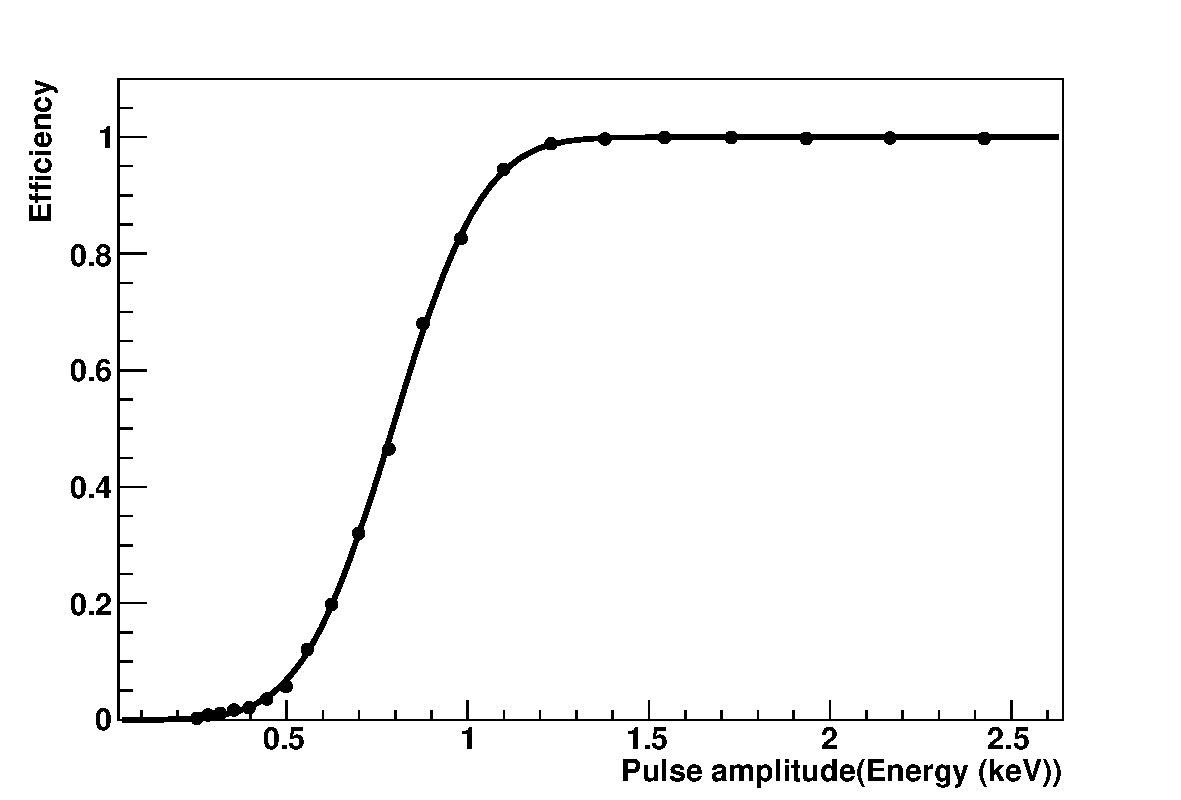
\includegraphics[width=0.7\textwidth]{EfficiencyExample}
					\caption[Triggering efficiency measurement example]
					{Triggering efficiency measurement example.  Line is a fit to 
					Equation~\ref{eqn:TriggerEfficiency}.}
					\label{fig:PPC2TriggeringEfficiencyExample}
				\end{figure}
	
			%%%%\begin{figure}
			%%%%	\centering
			%%%%	\subfigure[Scaling parameter, $s$, vs.~time.]{
			%%%%		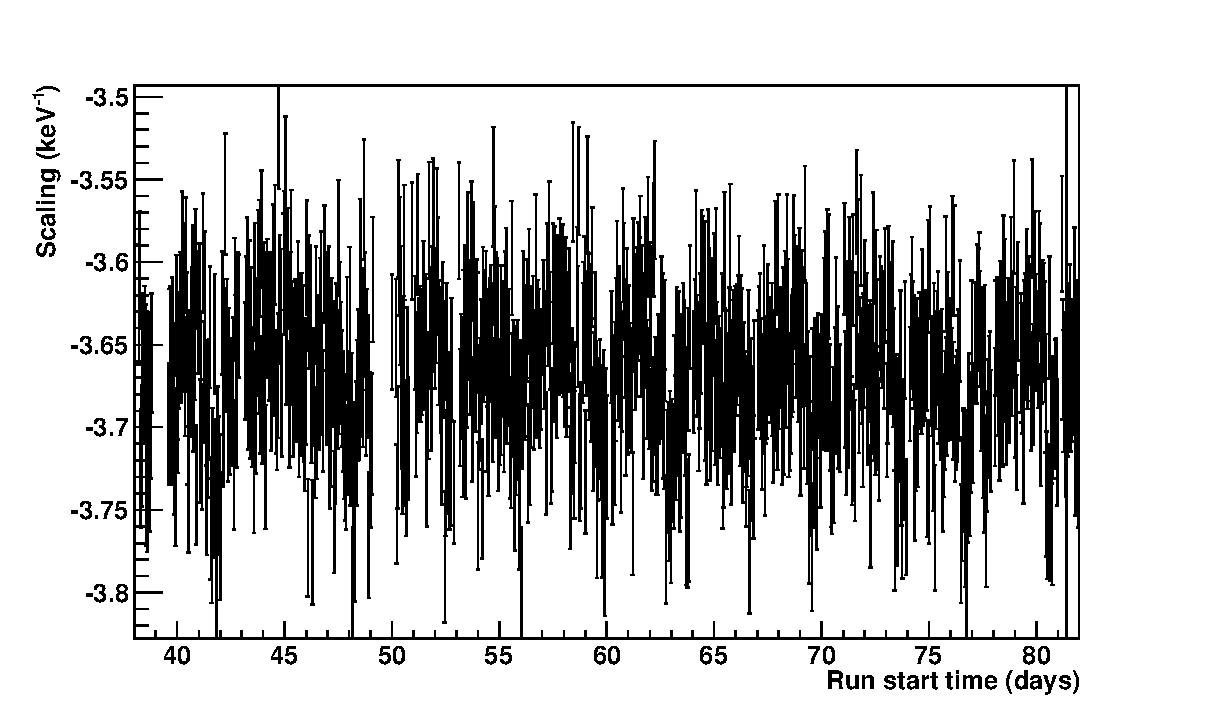
\includegraphics[width=0.45\textwidth]{ScalingVsRun0}
			%%%%		\label{fig:PPC2TriggeringEfficiencyTestsVsTimeScaling}
			%%%%	}
			%%%%	\subfigure[Offset parameter, $\sigma$, vs.~time.]{
			%%%%		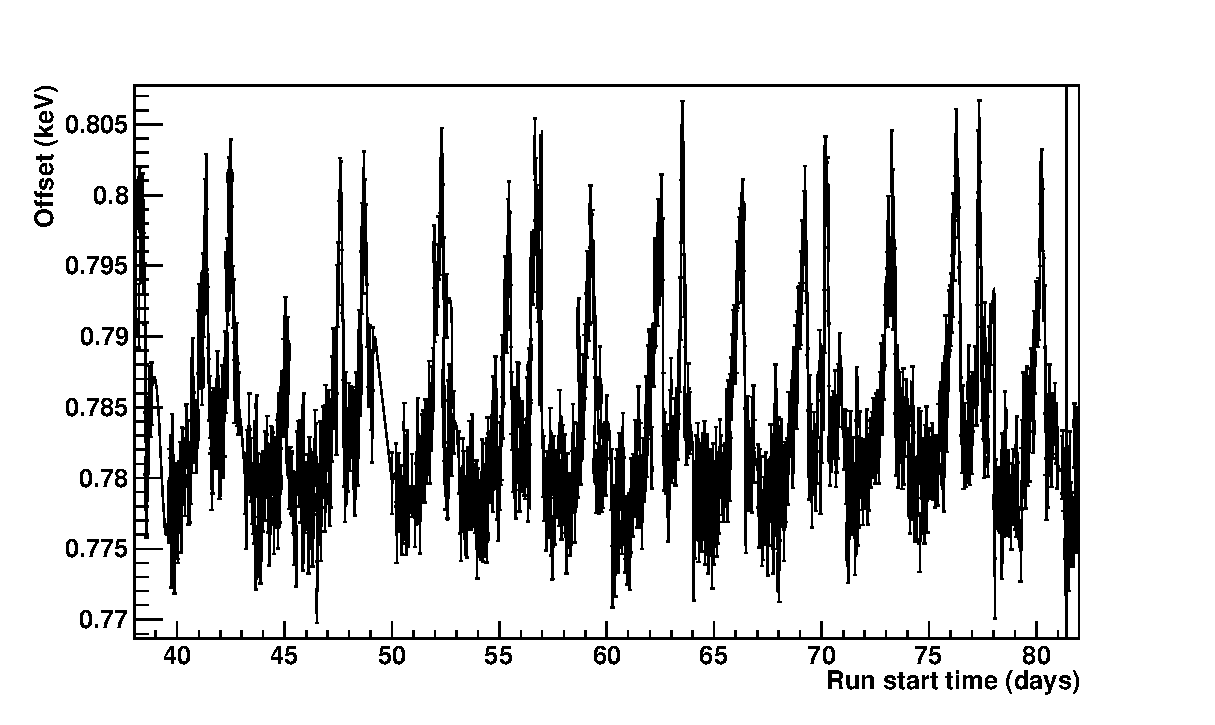
\includegraphics[width=0.45\textwidth]{OffsetVsRun0}
			%%%%		\label{fig:PPC2TriggeringEfficiencyTestsVsTimeOffset}
			%%%%	}						
			%%%%	\caption{Triggering efficiency tests vs. run time.  $\sim$5~min efficiency tests were run in 
			%%%%	between hour-long counting runs to measure how efficiency changed over time.}
			%%%%	\label{fig:PPC2TriggeringEfficiencyTestsVsTime}
			%%%%\end{figure}

			
				\begin{figure}
					\centering
					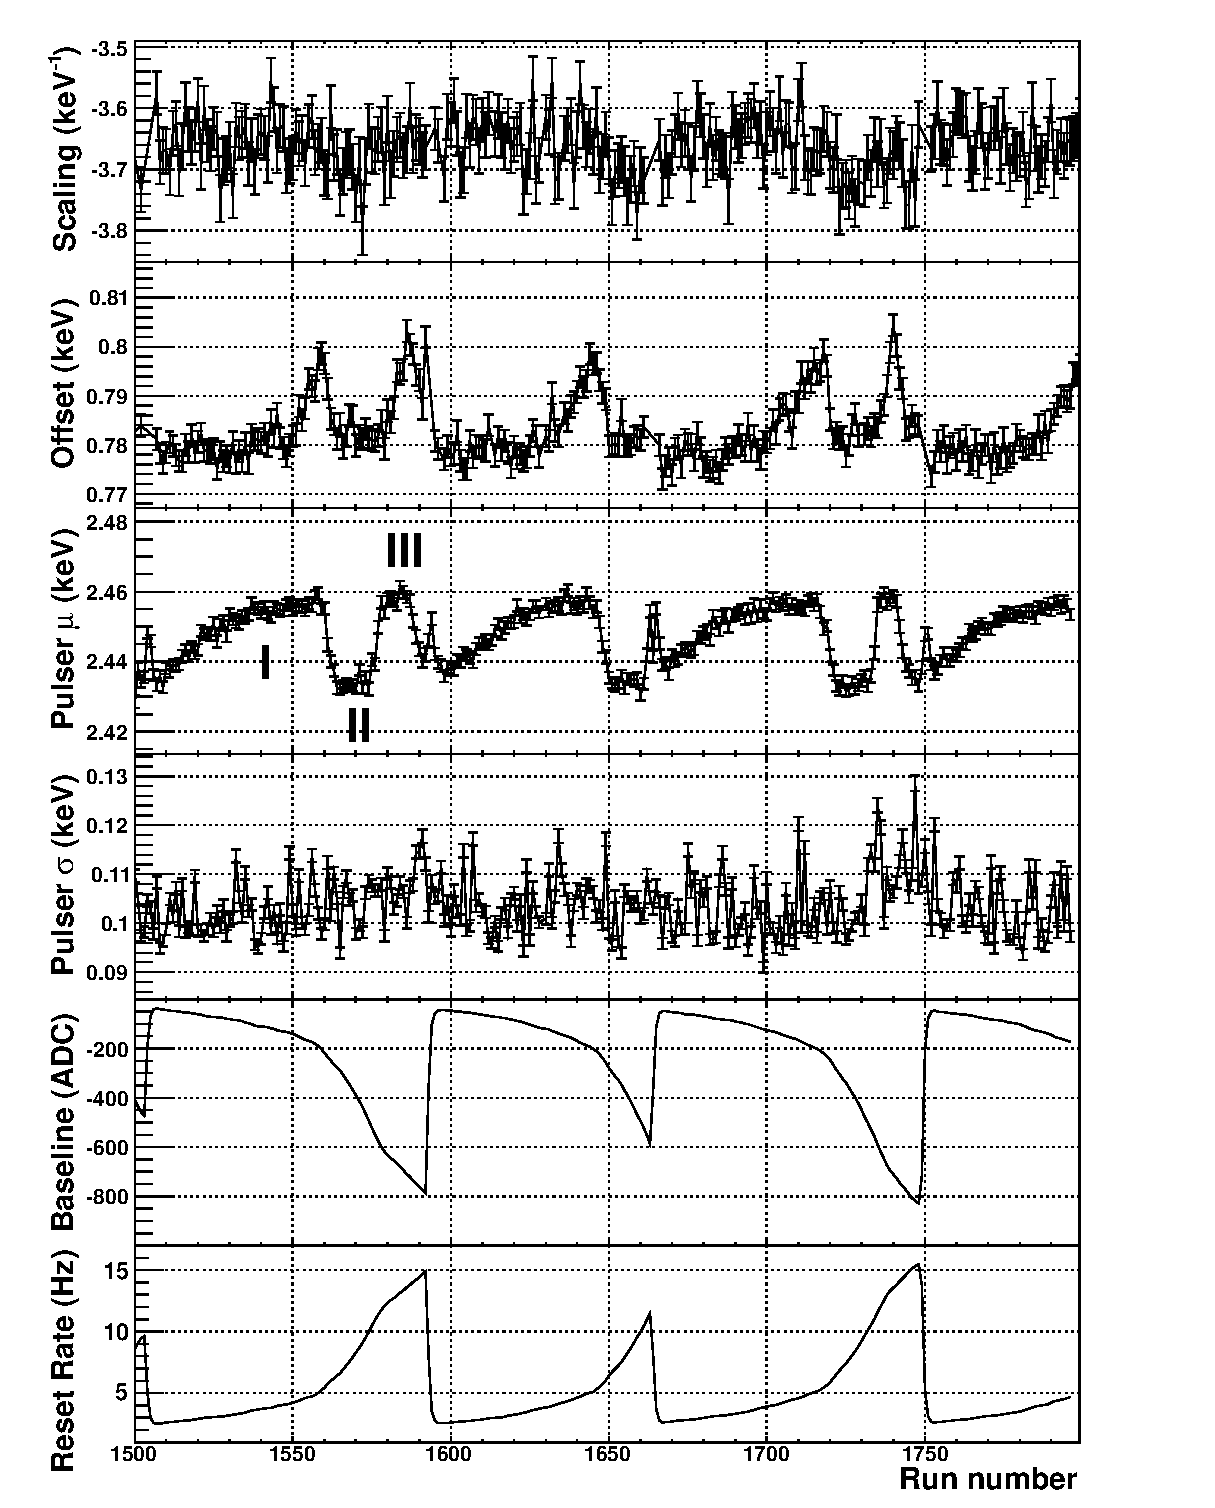
\includegraphics[width=0.95\textwidth]{AllPlotComparisons}
					\caption[Comparison of various parameters versus time for a subset of runs]
					{Comparison of various parameters versus time for a subset of runs.  See text for details.}
					\label{fig:PPC2AllPlotCompare}
				\end{figure}
	
	    	\subsubsection{Conclusions}
		\label{sec:DeploymentPPC2SoudanAnalysisParsTimeConclusion}    	
	
	The results of this section underscore the need to track detector parameters over time to monitor changing environmental conditions and other unanticipated behavior.  The gain and offset shifts evident in the pulser and trigger efficiency results do not significantly affect these data because their magnitudes ($<$25~eV) are much less than the nominal noise FWHM ($\sim$235~eV) and trigger threshold (90\% efficient at 1~keV) (see average values in Table~\ref{tab:PPC2AvgPars}).  However, these deviations could begin to have a larger effect with improved systems with reduced noise and threshold.  Additionally, when extracting information on physics signals in regions close to threshold (such as dark matter), it is critical to study parameters affecting this region over time to understand systematics important for limits or claims.  
	
				\begin{table}
					\centering
					\begin{tabular}{l r}
						\toprule
						Parameter & Value \\
						\midrule
						    \multicolumn{2}{c}{\emph{Pulser Data}} 	  \\
						    Mean, $\mu$ &  $2.45\pm0.009$ (keV) \\
						    Sigma, $\sigma$ &  $0.100\pm0.0046$ (keV) \\						    
						    \multicolumn{2}{c}{\emph{Trigger Efficiency}} 	  \\
						    Offset, $\rho$ &  $0.784\pm0.006$ (keV) \\
						    Scaling, $s$ &  $-3.666\pm0.044$ (keV$^{-1}$) \\						    						    
						\bottomrule
					\end{tabular}
					\caption[Average parameters for trigger efficiency and electronic noise]
					{Average parameters for trigger efficiency and electronic noise.}
					\label{tab:PPC2AvgPars}
				\end{table}	
	    	\subsection{Cuts}
		\label{sec:DeploymentPPC2SoudanAnalysisCuts}    
			
	Cuts were introduced to clean the data with the goal of removing spurious events from, for example, noise, microphonics and reset-pulse events.  These consisted of (1) a timing cut for removing reset pulse events, and (2) a baseline cut and (3) an integrated-counts-per-run cut for removing noise and microphonics-induced events.  The first two cuts were applied on an event-by-event basis, whereas the last cut removed an entire hour-long run. 
	
			\subsubsection{Reset-pulse timing cut}
	Reset pulse waveforms had distinct qualities (positive clipping whereas energy pulses were negative-going) which allowed the waveforms to be removed online from the data stream while retaining the timing information of the event.  The offline timing cut introduced a veto window of 1~ms following a reset event.  Given the average reset rate ($\sim$10~Hz), this introduced a $\sim$1\% correction to the live-time.  

			\subsubsection{Baseline cut}	
	The baselines of the traces were monitored on an event-by-event basis by calculating a 1st-degree polynomial fit to the first 3.5~$\mu$s of each preamp trace.  From this information, an average baseline was calculated for each run to generate a cut based upon significant deviations from these average values.  In a stable system, the baseline will be gaussian distributed around a central value according to the magnitude of the noise.  The integrated-counts-per-run in particular energy windows (0.6-10~keV and 10-70~keV) were monitored as well to observe deviations from expectation assuming poisson statistics.  This second cut relied upon the fact that spurious events from increases in environmental noise and microphonics arrive in bursts, see e.g.~\cite{Morales1992410}).  
	
	The average baseline per run shifted with a systematic correlation with a shift in the measured inhibit rate, shown in Figure~\ref{fig:PPC2AllPlotCompare}.  As the leakage current increased, the inhibit rate went up and the measured baseline dropped due to additional charge collection on the AC-coupling capacitor.  In general, this downward shift in baseline could affect the dynamic (energy) range of a digitizer channel because it would allow fewer ADC values for the (negative-going) pulses before clipping.  To generate a cut on this value, the values of the baseline for each event during a run were histogrammed and fit to a gaussian.  A cut was then generated based upon the results of this fit: rejecting events outside the range $\mu\pm3\sigma$ for a 99.7\% acceptance.  An example of one of these fits is shown in~\ref{fig:PPC2BaselineCuts}.  During LN fills, the baseline would return to its maximum value making a cut based upon the average baseline value impossible.  Runs during these transition times were cut from the data set.  
		
			%%%%\begin{figure}
			%%%%	\centering
			%%%%	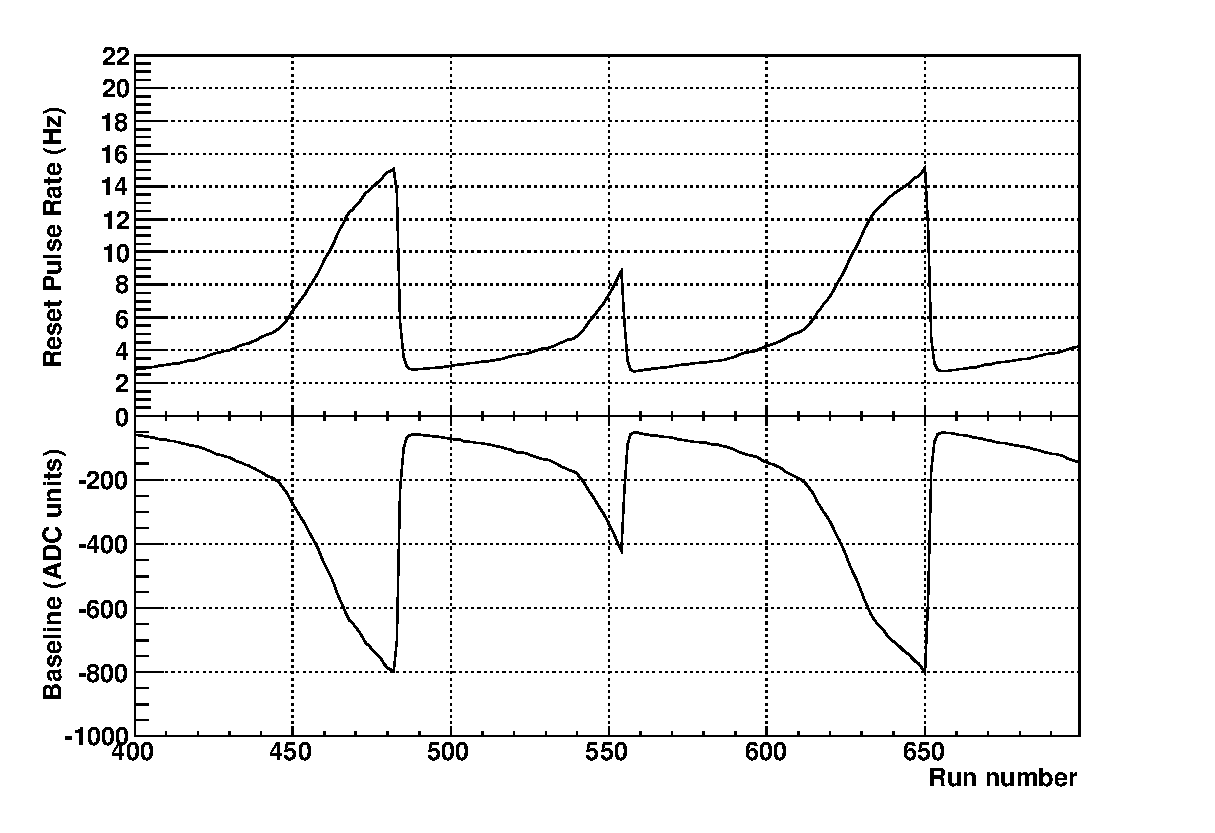
\includegraphics[width=0.9\textwidth]{BaselineVsRunNumberGraphPlot}
			%%%%	\caption{Measured baseline and inhibit rate versus run number for a subset of runs.}
			%%%%	\label{fig:PPC2BaselineInhibitRateVsTime}
			%%%%\end{figure}
						
				\begin{figure}
					\centering
					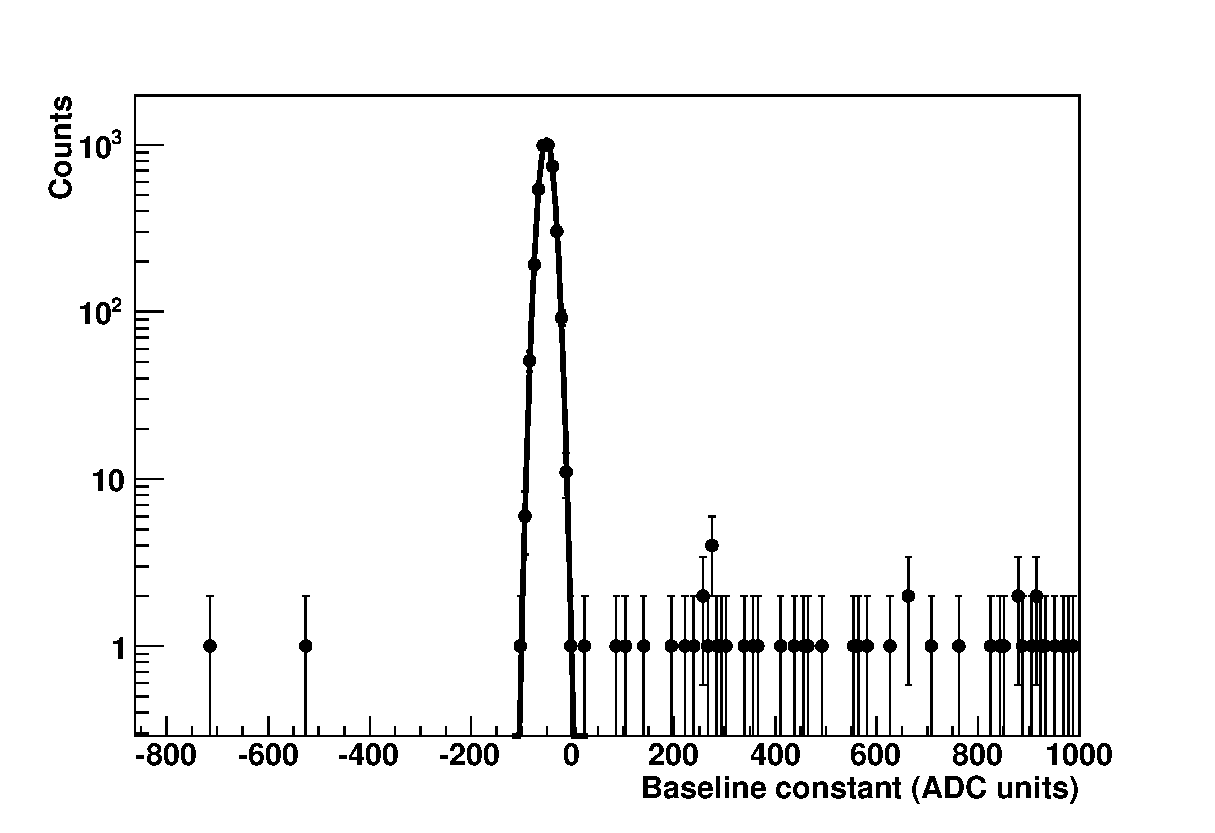
\includegraphics[width=0.7\textwidth]{BaselineExample}
					\caption[An example of a fit to the baseline for one hour-long run]
					{An example of a fit to the baseline for one hour-long run.  Line is a gaussian fit to the data.}
					\label{fig:PPC2BaselineCuts}
				\end{figure}
				
			\subsubsection{Integrated-counts-per-run cut}
	To determine the integrated-counts-per-run cut, counts in a designated energy window for each run were calculated and histogrammed.  The resulting data were then fit to a Poisson distribution and a cut was generated based upon 99.99\% acceptance using the fit distribution.  Results of this calculation are shown in Figure~\ref{fig:PPC2NoiseCuts}.  All runs with $\leq29$~counts between 0.6 and 10~keV were accepted.  
	
	All of these cuts were applied to the data to obtain a cleaned data set and all results described in the following sections use data after cuts.
	
				\begin{figure}
					\centering
					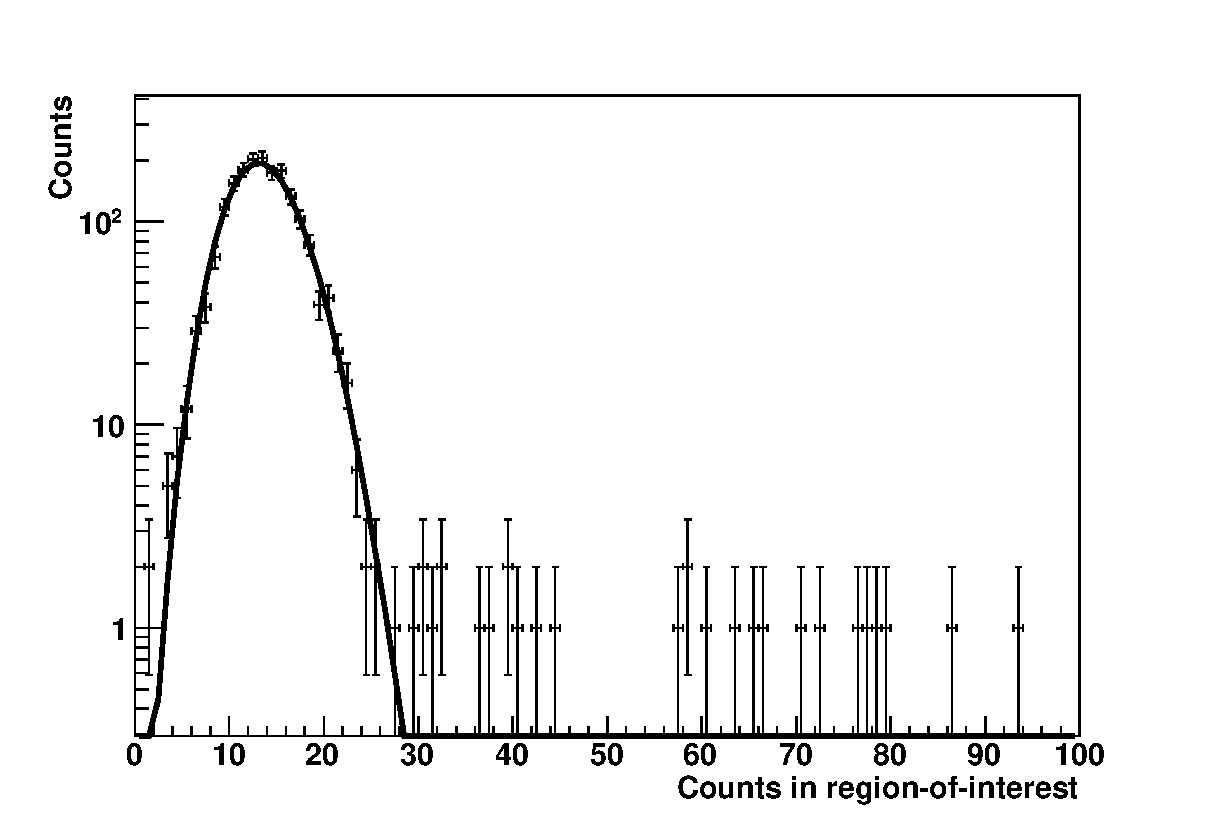
\includegraphics[width=0.7\textwidth]{LowROINoiseFit}
					\caption[Calculation of noise cuts]
					{Calculation of cut based upon the number of events in the energy window 0.6-10~keV per run.  
					The line is a fit to a Poisson distribution.  }
					\label{fig:PPC2NoiseCuts}
				\end{figure}
	
	    	\subsection{Rise-time calculations}
		\label{sec:DeploymentPPC2SoudanAnalysisRisetime}    
	
			
	The rise-time of each pulse was calculated using a simple algorithm: 
				\begin{enumerate}
					\item Subtract the baseline, $b$, and determine the amplitude, $a$.
					\item Forward search from beginning of the waveform to determine when the waveform reaches 
					$\frac{1}{2}a$ to find the middle of the pulse, $m$.
					\item From $m$, search backwards (forwards) to determine start (end) of the rise of the waveform.  
					The start and stop of the waveform are defined when the pulse reaches 10\% and 90\% of the amplitude.
				\end{enumerate}
The rise-time versus energy is plotted for each channel in Figure~\ref{fig:PPC2RisetimeCalculations}.  The low-gain channel demonstrates a sharp intensity band centered at $\sim$0.3~$\mu$s rise-time indicating that most pulses have this fast rise-time.  A number of gamma lines at higher energy are apparent in the data, including $^{40}$K (1460.8~keV), $^{214}$Bi (1764.5~keV), and $^{208}$Tl (2614.5~keV)\footnote{The thallium line is shifted in down in energy to $\sim$2550~keV.  An explanation of this is provided in Section~\ref{sec:DeploymentPPC2SoudanAnalysisEnergySpectra}}, with rise-time greater than~$0.3~\mu$s.  Because a large portion of events in these lines are composed of Compton-scatter interactions which deposit energy at multiple sites in the detector, this suggests multi-site events are being observed as slow-rise-time events.  
	
At low energy in the high-gain channel, one does not expect to see a significant multi-site population because Compton scatters summing to such a small energy are very improbable.  However, the rise-time distribution for the high-gain channel yields some interesting results: the strong line at $0.3~\mu$s still exists and there is a distribution near threshold ($\lesssim$1~keV) where it is clear the rise-time calculation algorithm breaks down, but there is also a strong population of slow-rise-time events at low energy, $1\leq E \leq20$~keV.  Closer inspection reveals a significant visual difference between `fast' ($\sim$0.3~$\mu$s) pulses and `slow' ($>1~\mu$s) pulses as can been seen in Figure~\ref{fig:PPC2RisetimeExamplePulses}.  A similar result was found for this detector by J.~Orrell~\cite{Orr2008a}.  Since these slow-rise-time events are predominately at low energy, they can compose a background to any signal near threshold.  See Section~\ref{sec:RisetimeCuts} for discussion on improved identification and removal of these events including a discussion on their potential origins.
	
				\begin{figure}
					\centering
					\subfigure[High-gain channel.]{
						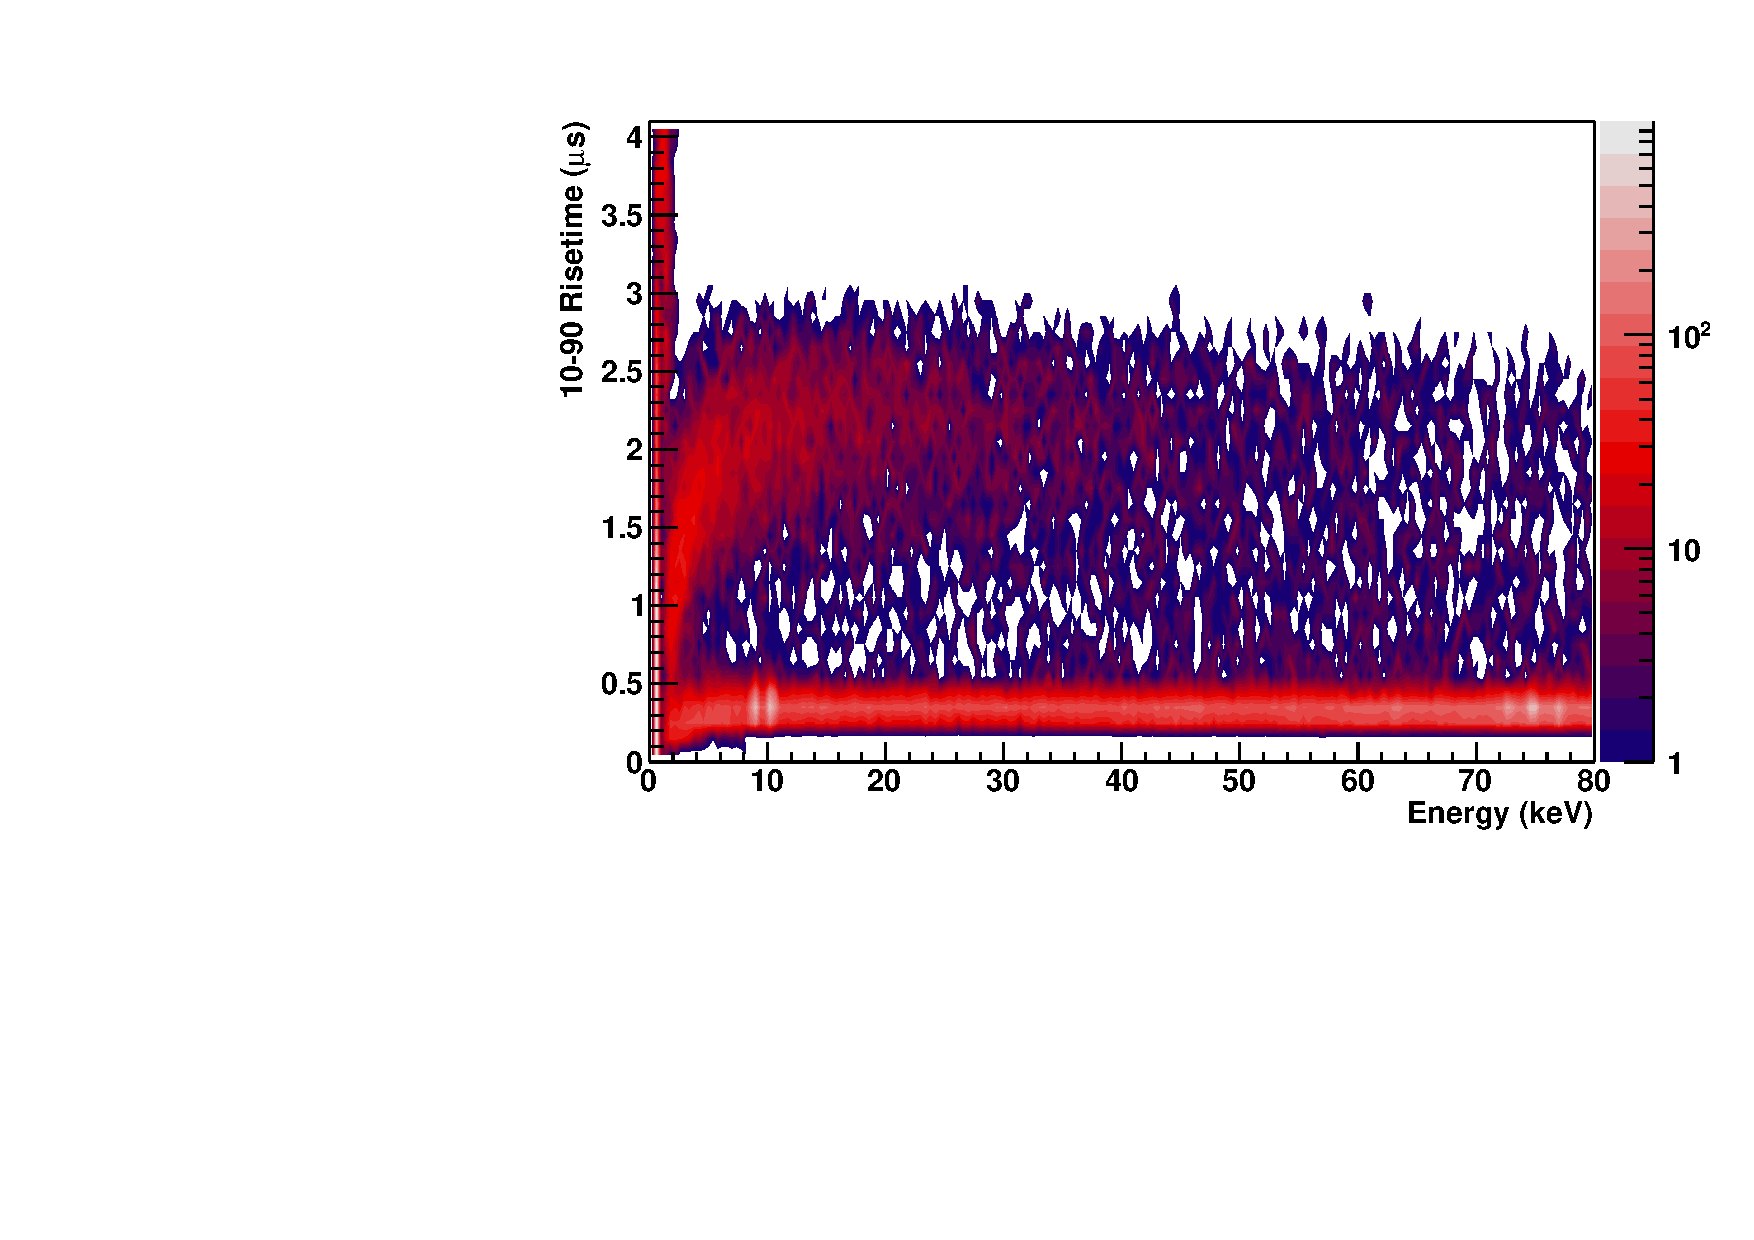
\includegraphics[width=0.8\textwidth]{RiseTimeVsEnergyChannel0}
						\label{fig:PPC2RisetimeCalculationsLow}
					}
					\subfigure[Low-gain channel.]{
						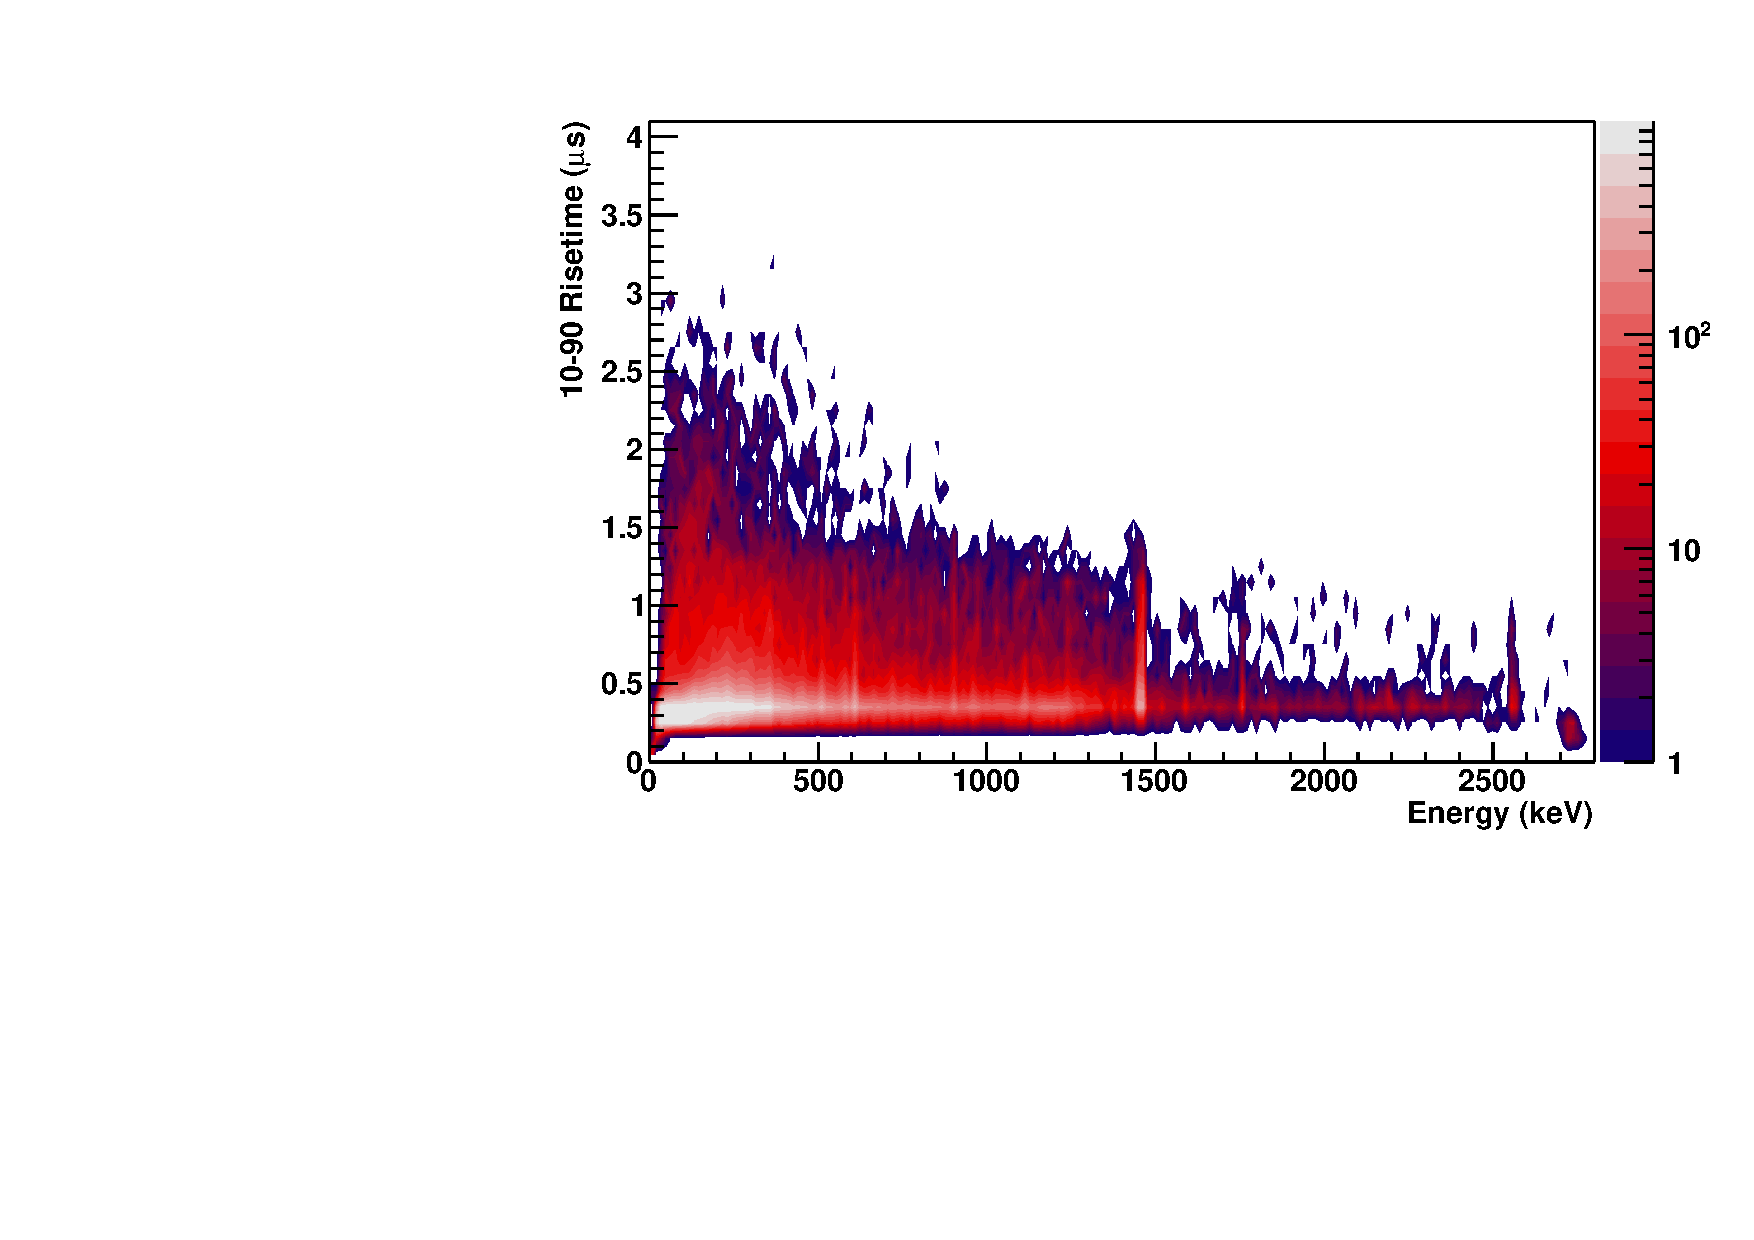
\includegraphics[width=0.8\textwidth]{RiseTimeVsEnergyChannel8}
						\label{fig:PPC2RisetimeCalculationsHigh}
					}	
					\caption[Rise-time measurements for high- and low-gain channels]
					{Risetime measurements for both high- and low-gain channels given in time from 10\%$\to$90\% 
					pulse amplitude.}
					\label{fig:PPC2RisetimeCalculations}
				\end{figure}		
	
				\begin{figure}
					\centering
					\subfigure[Fast pulse.]{
						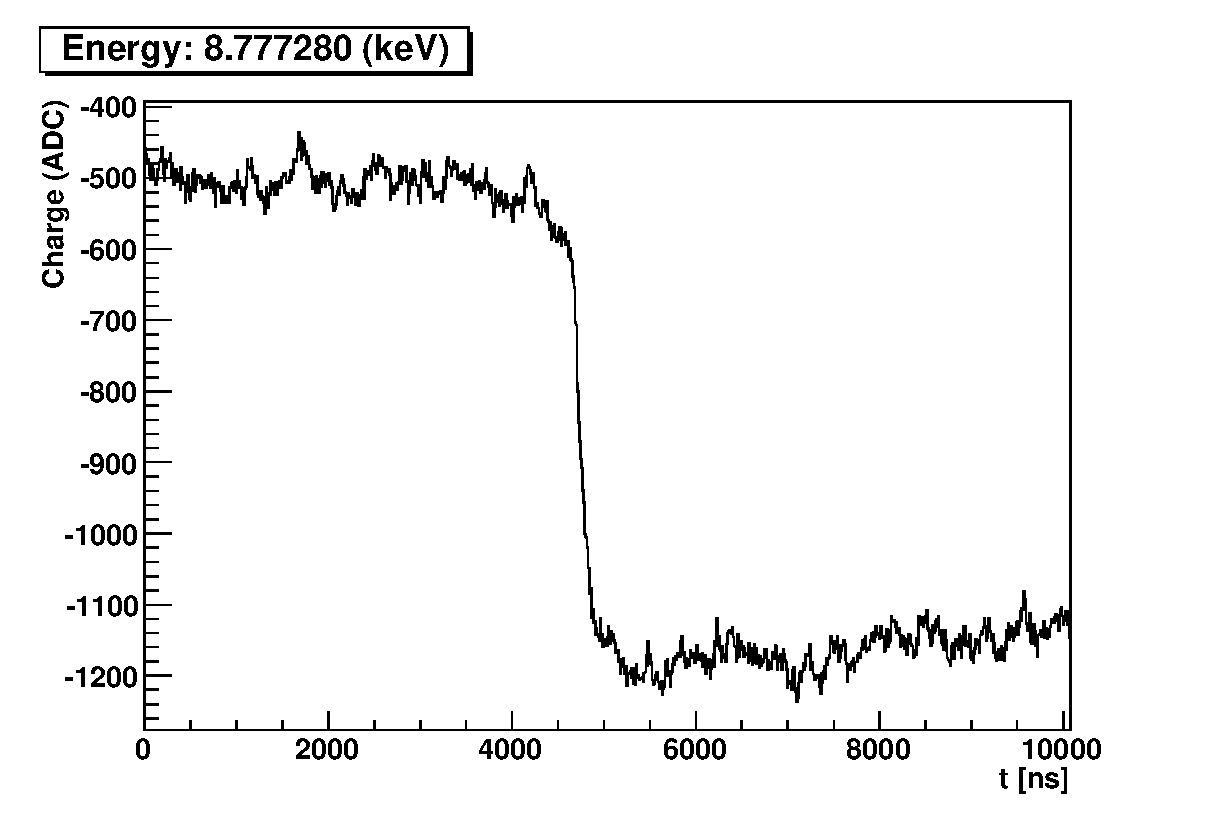
\includegraphics[width=0.45\textwidth]{fast_pulse_example}
						\label{fig:PPC2PulseExampleFast}
					}
					\subfigure[Slow pulse.]{
						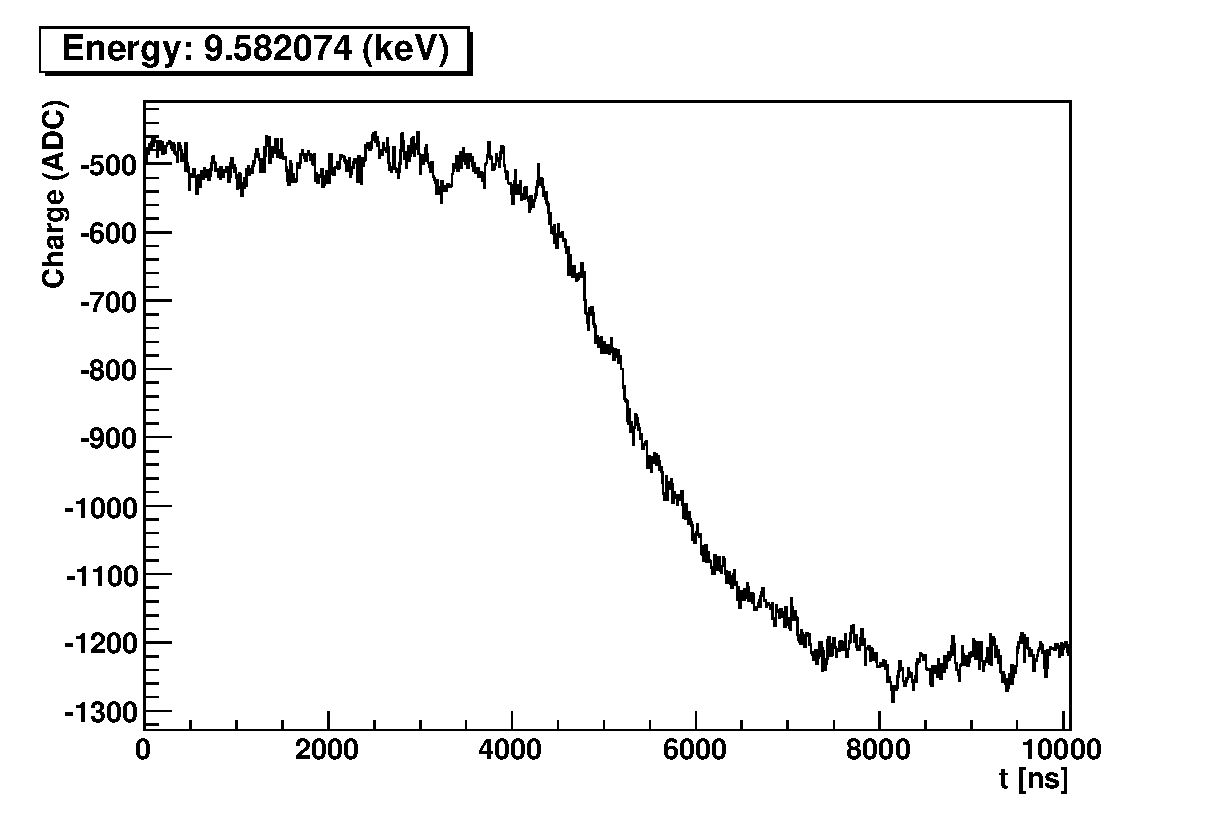
\includegraphics[width=0.45\textwidth]{slow_pulse_example}
						\label{fig:PPC2PulseExampleSlow}
					}					
					\caption[Examples of slow and fast rise-time pulses]
					{Examples of slow and fast rise-time pulses.}
					\label{fig:PPC2RisetimeExamplePulses}
				\end{figure}		
			
	    	\subsection{Energy spectra}
		\label{sec:DeploymentPPC2SoudanAnalysisEnergySpectra}    	
			
	Studies on the high-energy channel were performed by A.~Schubert to identify peaks and study the resolution of the detector with higher energy gamma lines~\cite{Schubert:2009ff}.  The spectrum was calibrated using prominent peaks in the spectra.  The resolution was fit to a second-order polynomial function of energy and determined to be:
				\begin{equation}
					\sigma = \sqrt{(0.242 \pm 0.016)^{2} +  E (4.04 \pm 0.1 \times 10^{-3})^{2} + E^{2} (9.2 \pm 0.0004 \times 10^{-4})^{2}} 
				\label{eqn:HighEnergySigma}
				\end{equation}			
with $E$, energy in keV.  It was found that the 2614.5~keV peak of the $^{208}$Tl decay was shifted down in energy to 2561~keV and had a larger-than-expected sigma (given Equation~\ref{eqn:HighEnergySigma}) of 8.6~keV.  This was explained by noting that large energy depositions in the crystal could saturate the pulse-reset preamp introducing either clipped or distorted pulses into the digitizer.  A selection of a few prominent lines fit in~\cite{Schubert:2009ff} is given in Table~\ref{tab:PPC2HighEnergyGammaLines}.  Results from this suggest that the linearity of the high-energy channel can not be trusted past the 1764~keV line of $^{214}$Bi.  This conclusion highlights a concern regarding the difficulty of using low-noise preamps with reset electronics while simultaneously looking at high-energy data $>$3-4~MeV as the \MJ~\minmod~will do.  Preamp solutions will have to address the optimization problem of ensuring enough dynamic range to search for $\nonubb$ while retaining low noise and threshold.  
	
				\begin{figure}
					\centering
					\subfigure[High-gain channel.]{
						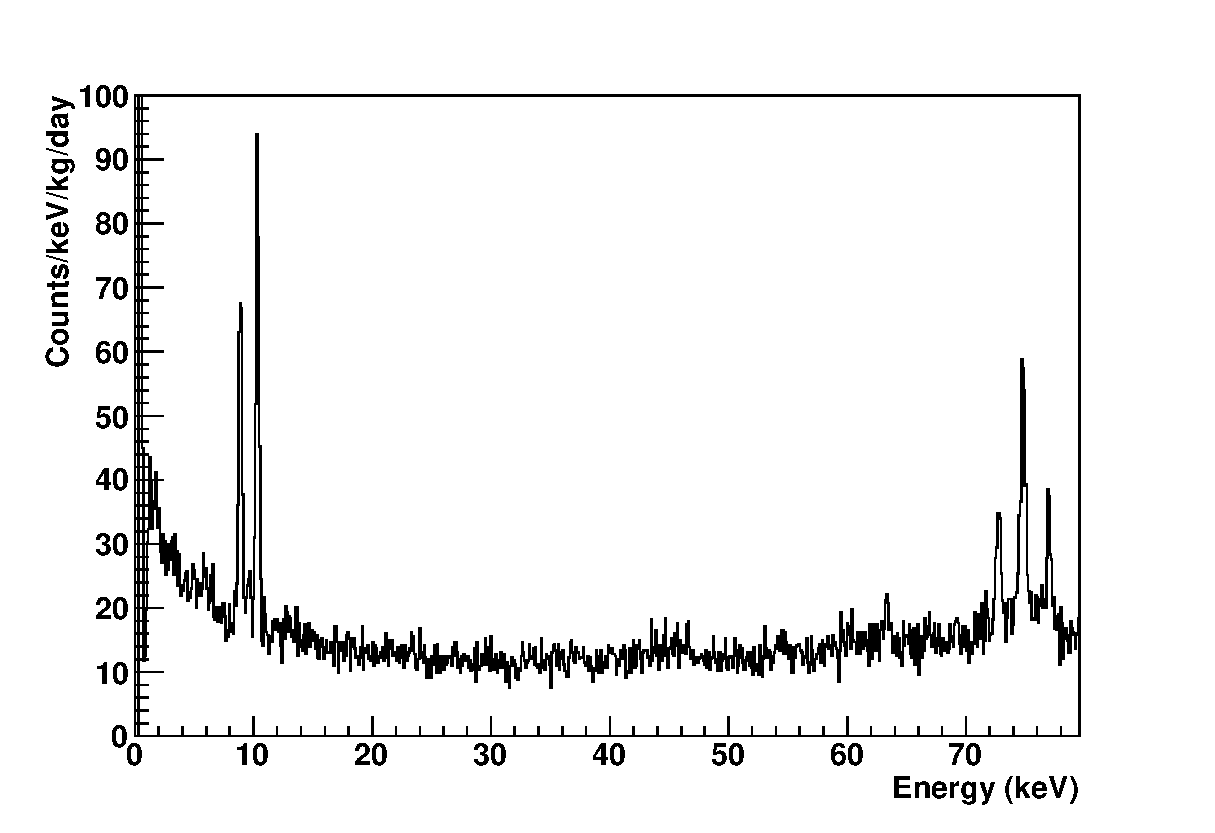
\includegraphics[width=0.8\textwidth]{LowEnergySpec}
						\label{fig:PPC2EnergySpecLow}
					}
					\subfigure[Low-gain channel.]{
						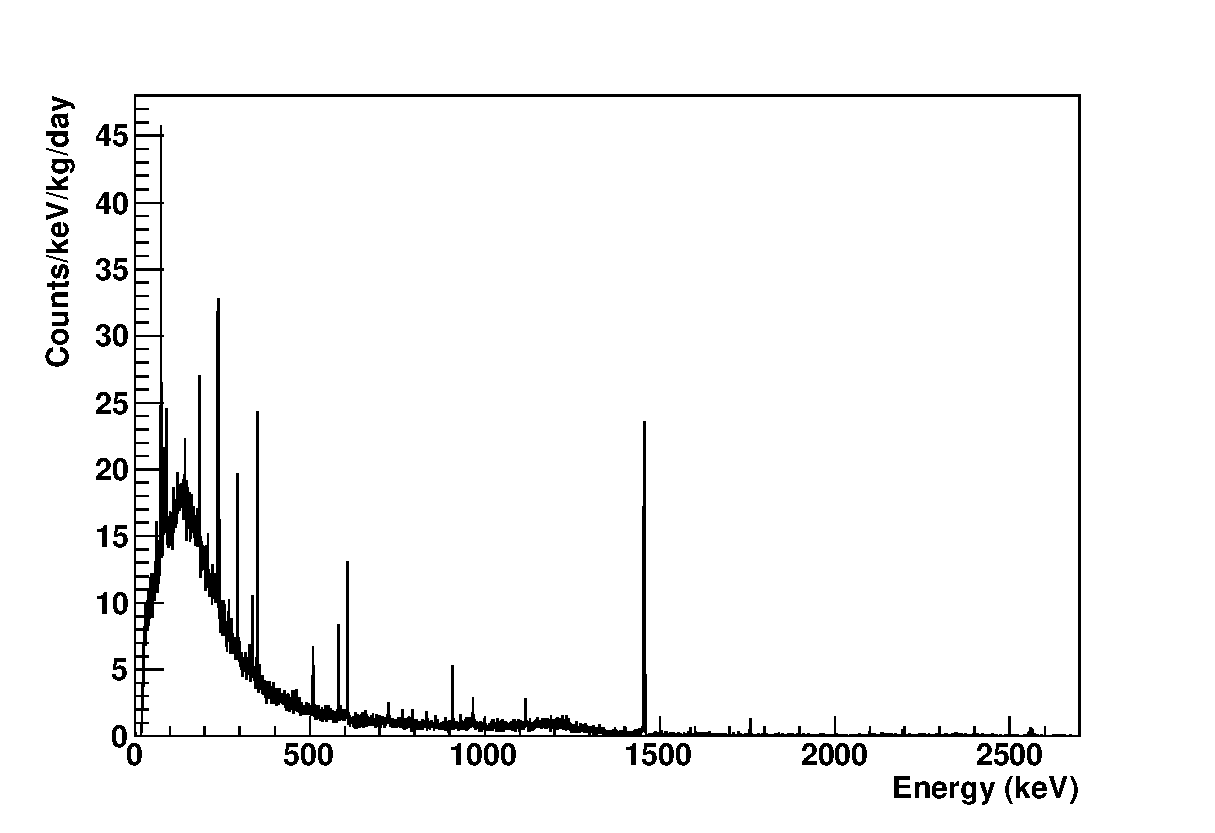
\includegraphics[width=0.8\textwidth]{HighEnergySpec}
						\label{fig:PPC2EnergySpecHigh}
					}
					\caption[Energy spectra of \ppc2.]
					{Energy spectra of \ppc2.}
					\label{fig:PPC2EnergySpectra}
				\end{figure}	
	
				\begin{table}
					\centering
					\begin{tabular}{  c  r  r  c  }
					\toprule
					{\bf Source} & {\bf Energy [keV]} & {\bf Fit centroid [keV]} & {\bf Sigma [keV]} \\  
					\midrule
					% fit of 1-degree polynomial continuum + 0 sawtooths + 1 gaussian(s) without  tail(s), wit\\
					$^{226}$Ra     & 186.2     ~ & 185.7      ${\pm}$ 0.04       ~ & 0.37       ${\pm}$ 0.03       \\
					% fit of 1-degree polynomial continuum + 0 sawtooths + 3 gaussian(s) without  tail(s), wit\\
					$^{212}$Pb     & 238.6     ~ & 238.5      ${\pm}$ 0.04       ~ & 0.32       ${\pm}$ 0.01       \\
					% fit of 1-degree polynomial continuum + 0 sawtooths + 3 gaussian(s) without  tail(s), wit\\
					$^{214}$Pb     & 242.0     ~ & 241.9      ${\pm}$ 0.04       ~ & 0.30       ${\pm}$ 0.06       \\
					% fit of 1-degree polynomial continuum + 0 sawtooths + 1 gaussian(s) without  tail(s), wit\\
					$^{214}$Pb     & 295.2     ~ & 295.1      ${\pm}$ 0.04       ~ & 0.41       ${\pm}$ 0.02       \\
					% fit of 1-degree polynomial continuum + 0 sawtooths + 1 gaussian(s) without  tail(s), wit\\
					$^{228}$Ac     & 338.3     ~ & 338.1      ${\pm}$ 0.04       ~ & 0.42       ${\pm}$ 0.04       \\
					% fit of 1-degree polynomial continuum + 0 sawtooths + 1 gaussian(s) without  tail(s), wit\\
					$^{214}$Pb     & 351.9     ~ & 351.7      ${\pm}$ 0.04       ~ & 0.38       ${\pm}$ 0.01       \\
					% fit of 1-degree polynomial continuum + 0 sawtooths + 1 gaussian(s) without  tail(s), wit\\
					$^{208}$Tl     & 583.2     ~ & 583.5      ${\pm}$ 0.04       ~ & 0.58       ${\pm}$ 0.03       \\
					% fit of 1-degree polynomial continuum + 0 sawtooths + 1 gaussian(s) without  tail(s), wit\\
					$^{214}$Bi     & 609.3     ~ & 609.6      ${\pm}$ 0.04       ~ & 0.60       ${\pm}$ 0.02       \\
					% fit of 1-degree polynomial continuum + 0 sawtooths + 1 gaussian(s) without  tail(s), wit\\
					$^{228}$Ac     & 911.2     ~ & 911.6      ${\pm}$ 0.1       ~ & 0.71       ${\pm}$ 0.06       \\
					% fit of 1-degree polynomial continuum + 0 sawtooths + 1 gaussian(s) without  tail(s), wit\\
					% fit of 1-degree polynomial continuum + 0 sawtooths + 1 gaussian(s) without  tail(s), wit\\
					$^{228}$Ac     & 969.0     ~ & 969.3      ${\pm}$ 0.1       ~ & 0.79       ${\pm}$ 0.10       \\
					% fit of 1-degree polynomial continuum + 0 sawtooths + 1 gaussian(s) without  tail(s), wit\\
					$^{214}$Bi     & 1120.3    ~ & 1120.5     ${\pm}$ 0.1       ~ & 1.03       ${\pm}$ 0.11       \\
					% fit of 1-degree polynomial continuum + 0 sawtooths + 1 gaussian(s) without  tail(s), wit\\
					$^{40}$K       & 1460.8    ~ & 1460.7     ${\pm}$ 0.04       ~ & 1.33       ${\pm}$ 0.02       \\
					% fit of 1-degree polynomial continuum + 0 sawtooths + 1 gaussian(s) without  tail(s), wit\\
					$^{214}$Bi     & 1764.5    ~ & 1764.3     ${\pm}$ 0.2       ~ & 1.72       ${\pm}$ 0.22       \\
					% sigma = sqrt( A^2 + energy*B^2 + energy^2*B^2 )\\
					% A = 1.8463 +/- 0.1859 E-1\\
					% B = 1.0921 +/- 0.2098 E-2\\
					% C = 8.4401 +/- 0.2725 E-4\\
					% 26 peaks were fit\\
					% chi-squared/dof: 83.3478 / 23.0000 ( 3.6238), p-val: 9.0378E-9\\
					% fit of 1-degree polynomial continuum + 0 sawtooths + 1 gaussian(s) without  tail(s), wit\\
					$^{214}$Bi     & 2204.2    ~ & 2201.5     ${\pm}$ 0.5       ~ & 1.94       ${\pm}$ 0.36       \\
					% sigma = sqrt( A^2 + energy*B^2 + energy^2*B^2 )\\
					% A = 1.8464 +/- 0.1857 E-1\\
					% B = 1.0918 +/- 0.2094 E-2\\
					% C = 8.4406 +/- 0.2711 E-4\\
					% 27 peaks were fit\\
					% chi-squared/dof: 83.3481 / 24.0000 ( 3.4728), p-val: 1.7660E-8\\
					% fit of 1-degree polynomial continuum + 0 sawtooths + 1 gaussian(s) without  tail(s), wit\\
					$^{208}$Tl    & 2614.5    ~ & 2560.6     ${\pm}$ 0.8       ~ & 8.59       ${\pm}$ 0.70       \\
					% fit of 1-degree polynomial continuum + 0 sawtooths + 1 gaussian(s) without  tail(s), wit\\
					% sigma = sqrt( A^2 + energy*B^2 + energy^2*B^2 )\\
					% A = 1.9182 +/- 0.1804 E-1\\
					% B = 9.5840 +/- 2.3753 E-3\\
					% C = 8.6656 +/- 0.2641 E-4\\
					% 29 peaks were fit\\
					% chi-squared/dof: 217.5429 / 26.0000 ( 8.3670), p-val: 3.7087E-32\\
					\bottomrule
					\end{tabular}

				
					\caption[Selection of gamma lines in the high-energy channel of \ppc2.]
					{Selection of gamma lines in the high-energy channel of \ppc2.  Table courtesy A.~Schubert.}
					\label{tab:PPC2HighEnergyGammaLines}
				\end{table}
	
	The calibration of the low-energy channel was refined using the \gersixeight~and \znsixfive~K-capture lines plus the non-overlapping x-ray lines from Pb and Bi (see the observed energy spectra in Figure~\ref{fig:PPC2EnergySpectra}).  The final maximum likelihood fits to these lines, means and sigmas and their expected value, are given in Table~\ref{tab:PPCLowEnergyLines}.  The x-ray lines from Pb and Bi come from the $\beta$-decays of $^{208}$Tl and $^{214}$Pb in the $^{232}$Th and $^{238}$U decay chains.  The two lines at $\sim$73~keV were fit with one gaussian which generated a wider width.  
				\begin{table}
					\begin{tabular}{l c c c}
						\toprule
						Source & Energy (keV) & Fit Mean (keV) & Fit Sigma (eV) \\
						\midrule						
						\znsixfive~K-capture & 8.979 & 8.95$\pm7.6\times10^{-3}$ & $139 \pm 7.3$ \\
						\gersixeight~K-capture & 10.367 & $10.394\pm5.8\times10^{-3}$ & $119 \pm 7.3$ \\
						$^{(208)}$Pb K$_{\alpha2}$ & 72.805 & $72.86\pm2.1\times10^{-2}$ & $188 \pm 19.7$ \\
						$^{(208)}$Pb K$_{\alpha1}$, $^{(214)}$Ba K$_{\alpha2}$ & 74.969, 74.815 & $74.92\pm1.3\times10^{-2}$ & $234 \pm 19.7$ \\
						$^{(214)}$Ba K$_{\alpha1}$ & 77.107& $77.11\pm1.9\times10^{-2}$ & $163 \pm 19.7$ \\		
						\bottomrule
					\end{tabular}
					\caption[Lines in the low-energy channel of \ppc2.]
					{Lines in the low-energy channel of \ppc2.}
					\label{tab:PPCLowEnergyLines}
				\end{table}

	\section{Estimate of \gersixeight~surface production}       
	\label{sec:Ge68ProdPPC}
	
       \gersixeight~is a cosmogenically-produced isotope inside germanium detectors which is a well-known background to $\nonubb$ (see e.g.~\cite{Ceb06aa}) due to the fact that the decays of its \galsixeight~daughters can deposit energy in the $\nonubb$ region-of-interest.  A schematic of the decay chain is shown in Figure~\ref{fig:GE68Decay}.  The decay of \gersixeight~proceeds via electron-capture with a half-life of 271~days to \galsixeight, which subsequently decays to $^{68}$Zn with a half-life of 68~minutes.  The latter decay has a Q-value of 2921~keV which could deposit energy at 2039~keV, the $\nonubb$ Q-value.  This background can be reduced two ways: (1) an analysis cut which tags the initial decay of \gersixeight~and vetoes the detector for a specified multiple of \galsixeight~half-lives, and/or (2) reduce the intrinsic \gersixeight~content in germanium detectors by either storing them in a low-cosmic-ray-flux environment (i.e.~underground) and waiting or by actively removing \gersixeight~through isotopic depletion.  Because \gersixeight~decays inside the detector, the total energy emitted through Auger electrons and x-rays is summed to lines of the K-, L-, or M-electron binding energy of the daughter nuclei (see Table~\ref{tab:GE68decayinfo}).  These lines can then be used to tag events likely to belong to a \gersixeight~decay.  Tagging the \gersixeight~decays to reduce the \galsixeight~background is dependent on the decay rate of \gersixeight, $\lambda^{(^{68}Ge)}$, and is not a viable solution until $\lambda^{(^{68}Ge)} \tau_{1/2}^{(^{68}Ga)} \ll 1$.   Estimations of the \gersixeight~activation rate at the earth's surface in both natural and enriched (86\% $^{76}$Ge) have been performed previously (see e.g.~\cite{Avi92,Elliott:2009cw}).  % FixME, second Elliott paper

       
       			\begin{table}
				\centering
				\begin{tabular}{ l c r }
					\toprule
					\gersixeight~decays & Percent & Energy (keV) \\
					\midrule
					     K-capture & $86.25\pm0.22$\% & 10.367 \\
					     L-capture & $11.45\pm0.20$ \% & 1.299 \\
					     M-capture & $1.92\pm0.08$\% & $\sim$0.1 \\
					\bottomrule
				\end{tabular}
				\caption[Decay information of\ \gersixeight]
				{Decay information of\ \gersixeight.  Capture probabilities are adapted from 
				reference~\cite{Schonfeld1994955}, characteristic energies from~\cite{Bea67}.}
				\label{tab:GE68decayinfo}
			\end{table}	
			\begin{figure}
				\centering
				\begin{tikzpicture}[node distance=0.4\textwidth]
		    			\node[circle] (GE68) {$^{68}$Ge};
					\node[circle, right of=GE68] (ga68) {$^{68}$Ga};
					\node[circle, right of=ga68] (zn68) {$^{68}$Zn};
					    
					\path[draw,->] (GE68) -- node[above] {\scriptsize $\epsilon$, T$_{1/2}=$271~d} (ga68);
					\path[draw,->] (ga68) -- node[above] {\scriptsize $\epsilon$, T$_{1/2}=$68~m, Q=2921~keV} (zn68);
					\draw (ga68) node[draw, rectangle, color=red, minimum height=0.1\textheight, minimum width=0.9\textwidth] {};
		 		\end{tikzpicture}
				\caption[Decay chain of $^{68}$Ge]
				{Decay chain of $^{68}$Ge.}
				\label{fig:GE68Decay}
			\end{figure}
			      
     The \ppc2 detector provided an excellent opportunity to measure the \gersixeight~activation rate at the surface.  Though the background rate at the L-capture energy of \gersixeight~was too high to resolve any peak, the K-capture line at 10.367~keV provided a means to measure the activation rate.  At the surface, the detector was assumed to be at equilibrium: that is, the decay rate of the cosmogenic isotopes were equal to the population rates.  This was a good approximation since the detector had been kept at the surface for a period on the order of the lifetime of \gersixeight.  Once the detector is brought underground, the cosmogenic isotopes are being populated at a rate much lower than that at the surface and it is a safe to assume at the depths of Soudan ($\sim2000$~m.w.e.) that this rate is 0.  Therefore, an underground measurement of the decay rate of \gersixeight~in counts/day can be used to determine the activation rate in counts/day at the surface.  The measurement was performed beginning 7~months after the detector had been deployed underground and after \gersevenone, a short-lived cosmogenic ($\tau_{1/2}=11.4$~days) which also populates the same capture peaks, had decayed.
		
	To perform the measurement, an energy window was selected around the K-capture peak from 10$\to$10.73~keV as the ``signal'' region -- chosen as symmetric around the expected signal mean -- and from 11$\to$15 as the ``background'' region, nearby and without any x-ray lines.  The average rate, in counts/keV/kg/day, was computed for each 72~hours of live-time in both regions and fit simultaneously to the function:
	
			\begin{equation}
				f(E,t) = \left\{ 
				\begin{array}{lr} 
 					a + b e^{-\left( \log{2} \right) t/\tau_{1/2}} & 10 \leq E \leq 10.73~\textrm{(keV)}\\
					\\
					a & 11 \leq E \leq 15~\textrm{(keV)}\\
				\end{array} \right.			
			\end{equation}
with the free parameters $a$ (flat background rate), $b$ (\gersixeight~rate), and $\tau_{1/2}$ (\gersixeight~half-life).  Fit results of this are summarized in Table~\ref{tab:Ge68FitResults} and plotted in Figure~\ref{fig:GE68Production}.  At the beginning of the counting runs, the detector had already been underground 212~days, meaning that the estimated decay rate, $b$, must be multiplied by the value $e^{(\log(2)~212 d/270.95 d)} = 1.72$ as well as  the energy window (0.73~keV) to get the counts-per-day-per-kilogram the day the detector was brought underground.  It was necessary to estimate the acceptance of the energy window using parameters ($\mu$ and $\sigma$) found from a maximum likelihood fit to the data (see, e.g.~Section~\ref{sec:DeploymentPPC2SoudanAnalysisEnergySpectra}); this acceptance was measured as $0.99797\pm0.001$.  Finally, since only the K-capture line was used in this estimation, the percentage of decays into this channel must be taken into account (see Table~\ref{tab:GE68decayinfo}).  The final result was then determined to be $53.3\pm4.3$~counts/kg/day which can also be interpreted as the activation rate for \gersixeight.  A comparison of this value to previous results is given in Table~\ref{tab:Ge68PreviousResults}.  It should be noted that this detector was fabricated in Europe and then shipped via airplane to Richland, WA, USA so that additional activation would have occurred during transportation.  Therefore, the calculated activation rate of $53.3\pm4.3$~\gersixeight~atoms/kg/day should be considered conservative since the detector would not have reached equilibrium from its original shipment date until its deployment underground ($\sim1$~year).

       			\begin{table}
				\centering
				\begin{tabular}{l r}
					\toprule
					Parameter & Fit Value \\
					\midrule
					$a$ & $16.166\pm0.33$ (counts/keV/kg/d)  \\
					$b$ & $36.54\pm2.94$ (counts/keV/kg/d)  \\
					$\tau_{1/2}$ & $192\pm96$ (days) \\
					$\chi^{2}$/NDF & 32.3/45 \\					
					\bottomrule
				\end{tabular}
				\caption[Fit information for \gersixeight~analysis]
				{Fit information for \gersixeight~analysis.}
				\label{tab:Ge68FitResults}	
			\end{table}	
			
			\begin{figure}
				\centering
				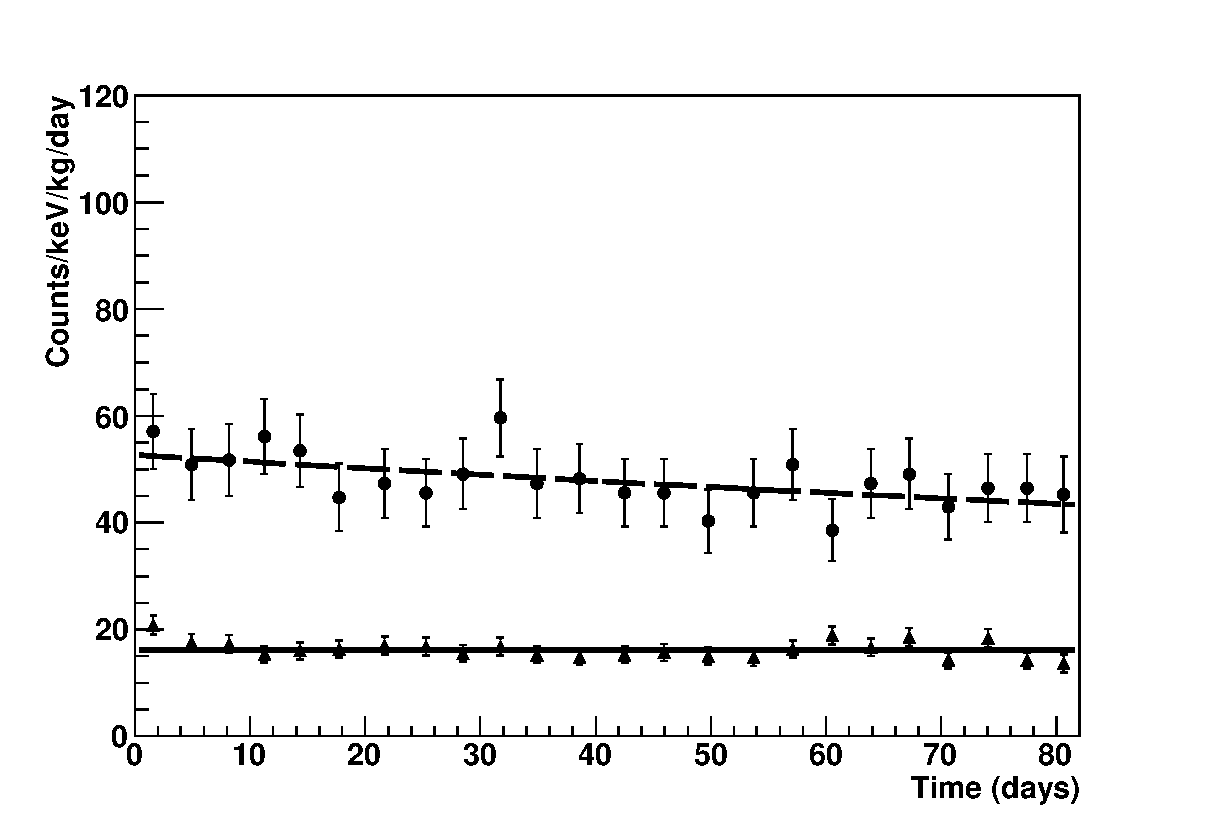
\includegraphics[width=0.7\textwidth]{G68_results}
				\caption[Estimation of $^{68}$Ge production at the surface]
				{Estimation of $^{68}$Ge production at the surface.  Data and fit for two regions:
				(1) 10$\to$10.73~keV, fit to exponential + constant (circles); and (2) 11$\to$14~keV, 
				fit to constant (triangles).  See text for fit details.}
				\label{fig:GE68Production}
			\end{figure}			
			
	          
	          	\begin{table}
				\centering
				\begin{tabular}{l r}
					\toprule
					Rate (\gersixeight~atoms/kg/day) & Reference \\
					\midrule
					29.6 (Calculation) & \cite{Avi92}\\
					$30\pm7$ (Experiment) & \cite{Avi92}\\
					58.4 & \cite{KlapdorKleingrothaus2002149}\\
					82.8 & \cite{Barabanov2006115}\\
					89 & \cite{Ceb06aa} \\
					45.8 & \cite{Back2008286}\\
					41.3 & \cite{Mei2009417}\\
					\bottomrule
				\end{tabular}
				\caption[Summary of previous estimates of \gersixeight~surface activation rates in natural Ge.]
				{A summary of previous estimates of \gersixeight~surface activation rates in natural Ge, 
				adapted from Table~1 in~\cite{Elliott:2009cw}.}
				\label{tab:Ge68PreviousResults}
	          	\end{table}			
			
	\section{Conclusions}
	
	A \MJ-like data acquisition system operated stably in a deployed environment for over a half year, demonstrating software and hardware robustness required for the \MJ~\minmod.  A tiered analysis framework was constructed that allowed automated processing and management of data from the deployed system.  This flexible framework was applied to data from two other detectors, including one analyzed in Chapter~\ref{chap:AnalysisBeGe}.  Several parameters of the data were tracked and exhibited deviations over time, underscoring the need to monitor channel rates, electronic noise, and trigger efficiency throughout the life of a deployed system.  Although the backgrounds seen in the detector were too large to provide competitive limits on dark matter signals, two important results from the data were made including a measurement of rise-time versus energy for low-energy pulses and an estimation of \gersixeight~surface activation in natural germanium.  The measurement of the former determined a potential source of background for applications such as the \MJ~\minmod~using PPCs for direct dark matter detection.  Results from this deployment reaffirmed conclusions made in Chapter~\ref{chap:DAQDevel}, namely that the trigger efficiency and electronic noise measured with this system were insufficient for dark matter searches or for sensitivity to the L-capture line of \gersixeight~and would require an update in hardware for improvement.

 
\clearpage

% ========== Chapter 4
 
\input{Chapters/AnalysisofDigitalBeGeData} 
\clearpage

% ========== Chapter 5
 
% In this chapter, I will perform calculations to determine
% sensitivity of Majorana, given the backgrounds discussed
% in the previous chapter, to dark matter and low-energy
% physics.  A number of different models of dark matter will be covered


% JFW has seen this and commented.  All comments incorporated, except for FixME statements.
\chapter{Limits on Light Weakly-Interacting Massive Particles (WIMPs)}
\label{chap:DMWIMPLimits}
	%\section{Calculating limits on a dark matter signal}
	%\label{sec:CalcLimitsOnDarkMatterSignal}

	As discussed in Chapter~\ref{chap:IntroChapter}, p-type point-contact detectors have sensitivity to low-mass WIMPs given their intrinsic low noise and low-energy thresholds.  This chapter presents the framework and methodology required for deriving limits on these particles given the data taken with the modified-\bege~detector at Soudan Underground Laboratory.  Emphasis is given on handling the difficulties described in the previous chapter related to unknown backgrounds at low energy.  

	\section{Signal from WIMP Dark Matter}
	\label{sec:CalcLimitsOnWIMPSignal}	

	A WIMP from the dark matter halo of the galaxy may interact with matter by recoiling off nuclei.  This interaction is in general dependent upon properties of the halo -- e.g.~density, escape velocity -- and characteristics of the detector -- e.g.~detector mass, atomic number.  The mathematical form has been derived in several reviews~\cite{Lew96,Jun96}.  The WIMP signal used in this analysis was the most generic parameterized form from Lewin and Smith~\cite{Lew96} given as a differential rate per recoil energy of the nucleus:

		\begin{eqnarray}
			\begin{aligned}
			\lefteqn{\frac{dR (v_{E}, v_{esc})}{dE_{rec}} = } \\ 
				& & \frac{k_{0}}{k_{1}} \frac{R_{0}}{E_{0} r} 
				\left\{ 
			 		\frac{\pi^{1/2}}{4} \frac{v_{0}}{v_{E}(t)} 
					\left[ 
						\operatorname{erf} \left( \frac{v_{min} + v_{E}(t)}{v_{0}} \right) - 
							   \operatorname{erf} \left( \frac{v_{min} - v_{E}(t)}{v_{0}} \right) 
					\right] 
					- e^{-v_{esc}^{2}/v_{0}^{2}} 
				\right\}
			\label{eqn:WIMPMasterEqn}
			\end{aligned}
		\end{eqnarray}
with 
		\[
		v_{E}(t) = v_{E_{0}} + v_{E_{1}}\sin (2 \pi t)
		\]
		\[
		\frac{k_{0}}{k_{1}} = \left[
			\operatorname{erf} \left( \frac{v_{esc}}{v_{0}} \right ) - 
			\frac{2}{\sqrt{\pi}} \frac{v_{esc}}{v_{0}} e^{-v_{esc}^{2}/v_{0}^{2}}
		\right]^{-1}
		\]
$R_{0}$ is related to the WIMP-nucleus cross section, $\signuc$ by:

		\[
			R_{0} = \frac{2}{\sqrt{\pi}} \frac{N_{A}}{A} \frac{\rho_{D}}{M_{W}} \signuc v_{0}
		\]
The above equations have a number of parameters which are described as follows:

		\begin{itemize}
			\item[$E_{rec}$]  -- Recoil energy of the nucleus. 
			\item[$E_{0}$] -- Energy of WIMP moving with velocity $v_{0}$
			\item[$r$] 	-- Dimensionless reduced mass given by 
					$\frac{4 M_{W} M_{T}}{(M_{W} + M_{T})^{2}}$
			\item[$v_{0}$] -- Velocity parameter in the Maxwellian velocity distribution of 
						the dark matter halo
			\item[$v_{min}$] -- Minimum WIMP velocity which can give a recoil energy $E_{rec}$
			\item[$v_{esc}$] -- Dark matter halo escape velocity
			\item[$v_{E_{0}}, v_{E_{1}}$] -- Parameters describing the velocity of the earth
			\item[$M_{W}$] -- Mass of a WIMP
			\item[$M_{T}$] -- Mass of a nucleus in the detector material
			\item[$A$] -- Atomic number of a nucleus in the detector material
			\item[$\rho_{D}$] -- Dark matter halo density	
			\item[$N_{A}$] -- Avogadro's number
			\item[$\signuc$] -- WIMP-nucleus cross section at zero velocity
		\end{itemize}			
This distribution is generally approximated using a single exponential in energy~\cite{Lew96}:
		\begin{equation}
\frac{dR (v_{E}, v_{esc})}{dE_{rec}} = 
				\frac{k_{0}}{k_{1}} \frac{R_{0}}{E_{0} r} 
				\left(  
					c_{1} e^{-c_{2}E_{R}/E_{0}r} 
					- e^{-v_{esc}^{2}/v_{0}^{2}} 
				\right)
		\end{equation}
 with constants, $c_{1}, c_{2}$ slightly varying with time.  The complete form (Equation~\ref{eqn:WIMPMasterEqn}) was chosen to allow eventually performing two-dimensional fits over both time and energy.  For these results the time dependence of the WIMP interaction is ignored and $t\to0$, which is an excellent approximation of the average of Equation~\ref{eqn:WIMPMasterEqn}.  

The WIMP-nucleus cross section is valid at small momentum transfers, $q = \sqrt{2 M_{T} E_{rec}}$, when $h/q$ is large compared to the size of the nucleus.  As the momentum transfer increases, the cross section for a coherent-nuclear-recoil interaction decreases.  This reduction in cross section is parameterized with a form factor to account for the dependence on momentum transfer: $\signuc \to \signuc F^{2} (q r_{n})$ where $r_{n}$ is the effective nuclear radius.  In this analysis, the Woods-Saxon/Helm form factor~\cite{Helm56} was used:

		\begin{equation}
			F (q r_{n}) = 3 \frac{j_{1}(q r_{n})}{q r_{n}} e^{-(q s)^{2}/s}
			\label{eqn:WSHelmFF}
		\end{equation}
with (from~\cite{Lew96})
		\[
			q r_{n} = \frac{\sqrt{2  M_{T} E_{rec}}}{197.3} 1.14 A^{1/3}
		\]
and $s$ is the nuclear skin thickness.  In practice, this correction is implemented by replacing all $\signuc$ with $\signuc F^{2}$ or, equivalently, by multiplying the differential rate by the form factor squared.  A plot of this form factor for germanium is shown in Figure~\ref{fig:HelmFF}, indicating that the form factor can provide a significant correction to the cross-section for ionization energies above $\sim10$~keV and a $\sim10$\% correction in the 0$\to$3~keV region.  

The WIMP-nucleus cross section, $\signuc$, is defined for a particular nucleus.  However, it is common to scale this parameter to a WIMP-nucleon cross section, $\sigman$, to compare between experiments using different detectors and therefore distinct nuclei.  The relationship from~\cite{Alner2005444} is given as: 
		\begin{equation}
			\sigman = \left( \frac{\mu_{1}}{\mu_{A}} \right)^{2}\frac{1}{A^{2}} \signuc 
			\label{eqn:SigmaConversion}
		\end{equation}
where $\mu_{A} = \frac{M_{W} M_{T}}{M_{W} + M_{T}}$ and $\mu_{1}$ is defined at $A=1$.  All exclusion plots will be presented in terms of $\sigman$, but all other results will be presented in terms of $\signuc$.

		\begin{figure}
			\centering
			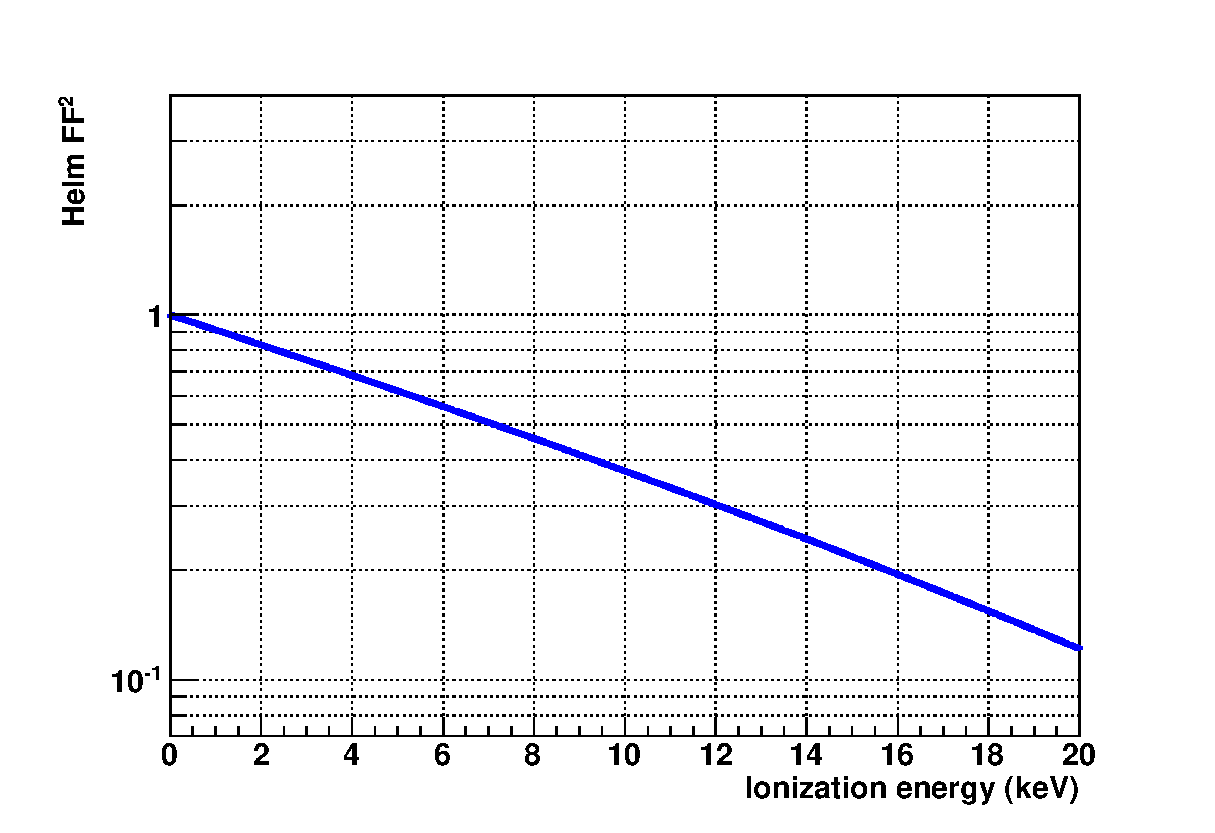
\includegraphics[width=0.7\textwidth]{HelmFormFactor}
			\caption[A plot of the Ge form factor versus ionization energy]
			{A plot of the Ge form factor versus ionization energy.  For a discussion of the 
			conversion from nuclear recoil energy to ionization energy, see 
			Section~\ref{sec:ResultsQuenching}.}
			\label{fig:HelmFF}.
		\end{figure}
	\section{Quenching}
	\label{sec:ResultsQuenching}
In ionization detectors, the calibration relating the energy deposited per
amount of charge collected is generally performed by using gamma lines from a
known source.  However, since photons interact by recoiling off electrons in
the detector, this calibration is only valid for other processes which deposit
energy in a similar manner.  In contrast, a particle that deposits energy in a
detector by recoiling off a nucleus (such as a WIMP) does not
generate the same amount of charge per amount of energy deposited as an
electron-recoil interaction.  The relationship between the `seen' ionization
from a nuclear recoil and the `seen' ionization from an electron recoil at the
same energy is referred to as quenching.  For ionization detectors, a theory
has been developed by Lindhard et al.~\cite{Lindhard:1961fa} to parameterize
this relationship:

		\begin{equation}
			E_{ion} =  \frac{k E_{rec} g(\epsilon)}{1 + k g(\epsilon)}
			\label{eqn:LindhardFunction}
		\end{equation}
with 
		\begin{eqnarray*}
			g(\epsilon) & = & 3 \epsilon^{0.15} + 0.7\epsilon^{0.6} + \epsilon \\		
			\epsilon & = & 11.5 E_{rec} Z^{-7/3} \\
		\end{eqnarray*}
For germanium detectors, the constant, $k$, has been recently estimated as 0.2 by Barbeau, et al.~\cite{Barbeau:2009fk} in the energy region $\lesssim4$~keV.  In a single-mode readout detector (e.g.~reading out \emph{only} ionization), nuclear recoil and electron recoil events are indistinguishable and so it is necessary to transform all theoretical spectra defined in recoil energy to ionization energy.  Unfortunately, accomplishing this requires inverting the Lindhard equation which is impossible to do analytically and so it essential to either obtain it numerically or to estimate this function with another function.  The function $E_{ion} =  \alpha E_{rec}^{\beta}$ provides an excellent approximation to this equation and can be easily inverted and differentiated.  Results from a fit of this function to the Lindhard equation (Eqn.~\ref{eqn:LindhardFunction}) for germanium detectors are shown in Figure~\ref{fig:LindhardFitResults}.  Fit values for $\alpha$ and $\beta$ are $0.204971$ and $1.13615$, respectively.

		\begin{figure}
			\centering
			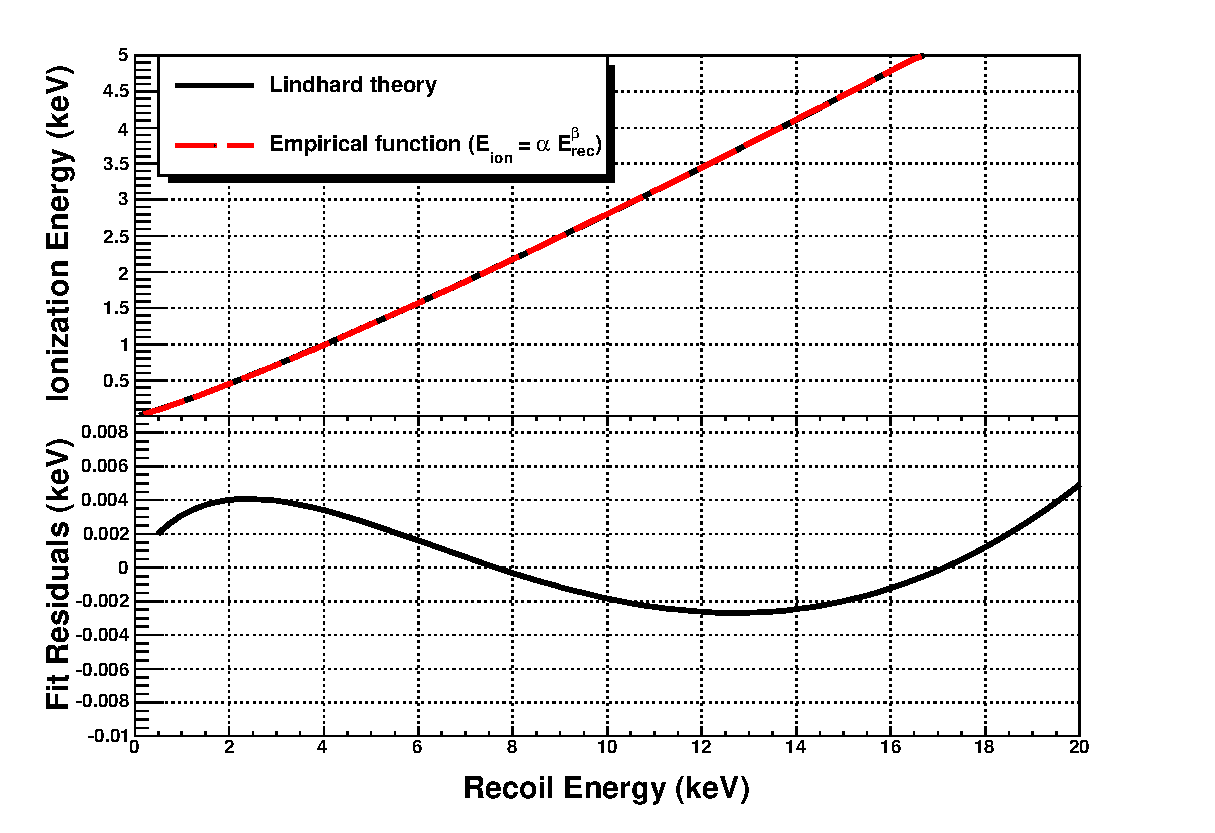
\includegraphics[width=0.7\textwidth]{quenching}
			\caption[Lindhard function with a fit to $E_{ion} =  \alpha E_{rec}^{\beta}$]
			{Lindhard function with a fit to $E_{ion} =  \alpha E_{rec}^{\beta}$.  
			The bottom plot displays the residuals, 
			indicating that the estimating function is good to better than 1\% in the 
			ionization energy range 0.5$\to$3.5~keV.}
			\label{fig:LindhardFitResults}
		\end{figure}
Combining this all together to determine the WIMP time and energy spectrum in terms of ionization energy yields the final differential rate:
		\begin{equation}
				\frac{dR}{dE_{ion}}  = \left(\frac{dR}{dE_{rec}} \right) \left(\frac{dE_{rec}}{dE_{ion}} \right) F^{2}
			\label{eqn:FinalFitSpectrum}
		\end{equation}	
A summary of the parameters used is given in Table~\ref{tab:BeGeFitParameters}.  The effect of including the escape velocity and the form factor for a low-mass (10~GeV) WIMP is shown in Figure~\ref{fig:1DDMSignal} where $t=0$.  This plot demonstrates the importance of a low threshold for detecting low-mass WIMPs since the escape velocity effectively truncates the WIMP spectrum above a certain energy.  Therefore, count rates for low-mass WIMPs become negligible for detectors with high enough thresholds.  The small correction from the form factor can be seen as a reduction in the count rate.  An example two-dimensional (energy and time) WIMP spectrum is shown in Figure~\ref{fig:2DDMSignal}.  In both of these plots, the differential rate is divided by the WIMP-nucleus cross-section.

		\begin{table}
			\centering
			\caption[Summary of parameters used in the WIMP exclusion fits]
			{Summary of parameters used in the WIMP exclusion fits.}
			\label{tab:BeGeFitParameters}
			\smallskip
			\begin{threeparttable}
				\begin{tabular}{l r}
					\toprule
					Parameter & Value (unit) \\
					\midrule
					\multicolumn{2}{l}{\emph{Fit parameters}} \\
					Atomic Mass & 72.96 (amu) \\
					$\rho_{D}$  &  0.4 (GeV cm$^{-3}$) \\
					Average velocity, $v_{0}$ & 230 (km s$^{-1}$) \\
					DM escape velocity, $v_{esc}$ & 600 (km s$^{-1}$) \\
					Velocity of the earth, $v_{E_{0}}$ & 244 (km s$^{-1}$) \\
					%Variational velocity of the earth, $v_{E}_{1}$\footnote{Not used in this fit} & 15 km s$^{-1}$ \\
					Detector mass &  0.33, 0.4\tnote{a} (kg) \\
					Nuclear skin thickness $s$ & 0.9 (fm) \\
					\multicolumn{2}{l}{\emph{Data set limits}} \\					
					Threshold & 0.5 (keV) \\
					Max energy & 3.5 (keV) \\					
					\bottomrule
				\end{tabular}	
				 \begin{tablenotes}
				       \item[a] {The smaller mass value is used when rise-time cuts are applied, see 
				       Section~\ref{sec:RisetimeCuts}.}
			     	\end{tablenotes}
			\end{threeparttable}
		\end{table}
		\begin{figure}
			\centering
			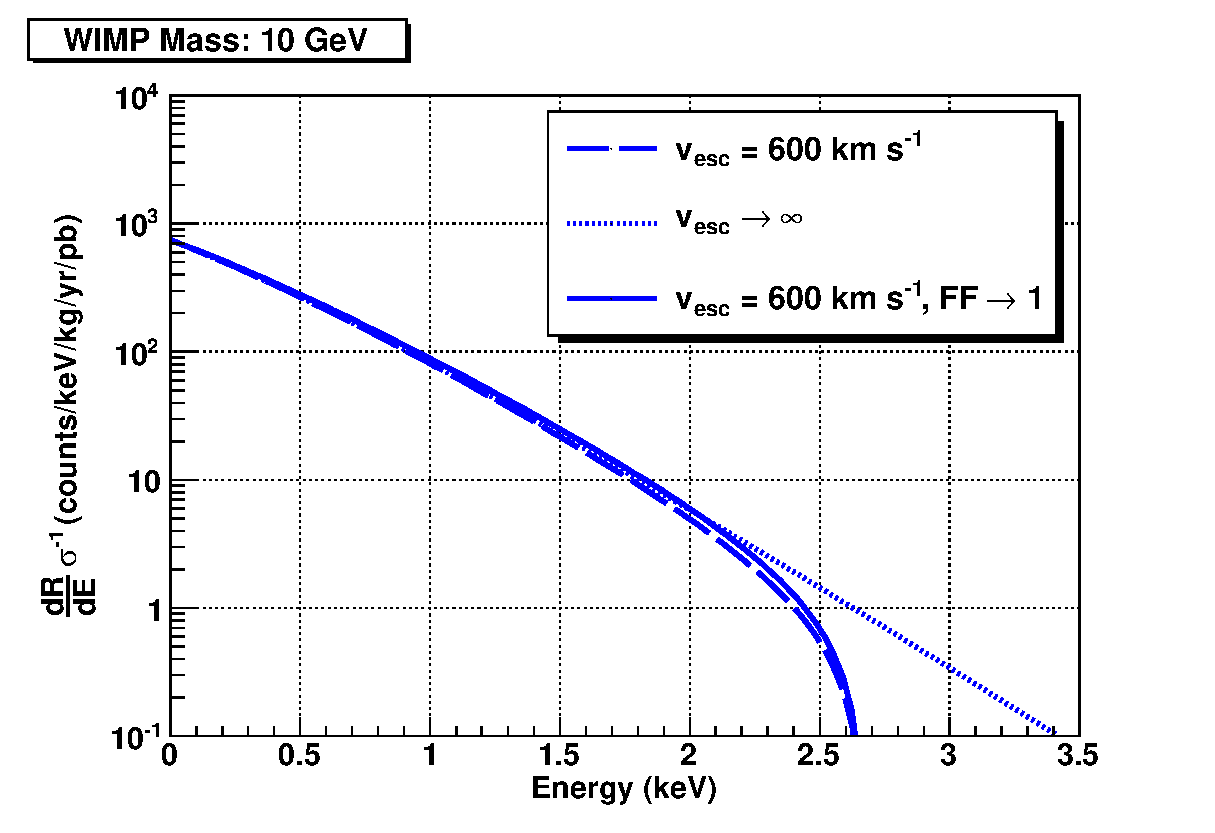
\includegraphics[width=0.9\textwidth]{WIMPMass10GeVExample}
			\caption[Count rate/cross section vs.~ionization energy for a 10~GeV WIMP]
			{Count rate/cross section vs.~ionization energy for a 10~GeV WIMP for 3 different model 
			variations: (1) Finite escape velocity and Helm form factor, (2) infinite escape velocity, 
			and (3) finite escape velocity and a form factor of 1.}
			\label{fig:1DDMSignal}
		\end{figure}
		
		\begin{figure}
			\centering
			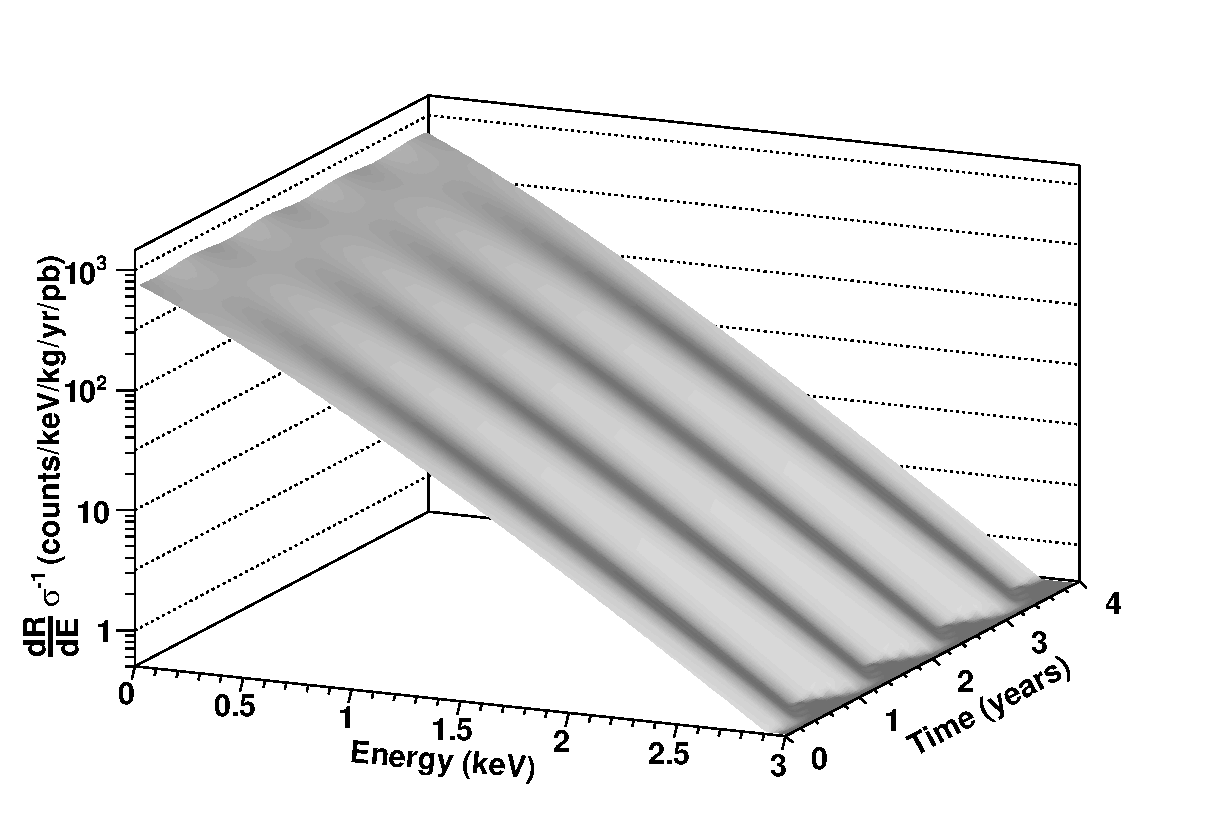
\includegraphics[width=0.9\textwidth]{WIMPModel}
			\caption[2-dimensional WIMP dark matter signal]
			{2-dimensional WIMP dark matter signal, $M_{WIMP} = $10~GeV.}
			\label{fig:2DDMSignal}
		\end{figure}


\section{Fit Methodology} 

	The analysis of the modified-\bege~data presented in the previous chapter, in particular Section~\ref{sec:BeGeLowEnergyFeatures}, uncovered several difficulties which must be addressed when determining limits with the data.  This section discusses the extraction of a signal limit using the maximum-likelihood method and explores the necessary mechanisms for dealing with unknown backgrounds.  
	
	\subsection{Obtaining Limits Using Maximum Likelihood}
	\label{sec:LimitsML}		

A maximum-likelihood analysis provides a mechanism for estimating the parameters of a model given a set of data.  There also exist standard techniques within the maximum-likelihood framework for hypothesis testing or searching for and generating limits on a signal that may exist in the data set.  In contrast to using $\chi^{2}$-minimization for parameter estimation, maximum likelihood does not require the binning of data
% though it does accommodate it
 and it does not provide a mechanism for estimating the goodness-of-fit.  The procedure for determining the set of parameters which best describes a data set involves constructing a likelihood function as the following:
		\begin{equation}
		L = \prod^{n} f({\tbf}, x_{n})
		\label{eqn:loglikelihood}
		\end{equation}
where $f(\theta, x)$ is a probability distribution function (pdf) describing the data, $x_{n}$, with parameter set $\tbf$.  The true values of the parameters, $\boldsymbol{\theta_{T}}$, are then estimated by maximizing $L$, or, equivalently, by minimizing $-\log L$.  For some more-trivial pdfs, it is possible to find an analytical solution to the equation set: $-\frac{\partial ( \log L )}{\partial\tbf} = 0$, but normally the minimization of the function is handled numerically.  

Hypothesis testing defines a mechanism by which one compares two models to the same data to find the favored model.  It is useful when searching for limits on a signal since one can compare the null hypothesis (no signal) versus the model with signal included.  Hypothesis testing using likelihood functions is performed by using a profile-likelihood test which involves the construction of a profile-likelihood function over a parameter or set of parameters, $\theta_{0}$:
		\begin{equation}
		\lambda(\theta_{0}) = \log L_{max}  - \log L_{max}(\theta_{0}, \boldsymbol{\theta_{n}})
		\end{equation}
assuming that $\theta_{0}$ is a subset of $\tbf$, or $\tbf = \{\theta_{0}, \boldsymbol{\theta_{n}}\}$.  $L_{max}$ is the likelihood function maximized for all parameters, and $ L_{max}(\theta_{0}, \boldsymbol{\theta_{n}})$ is the likelihood function at parameter value $\theta_{0}$ maximized over all other parameters except $\theta_{0}$.  The profile-likelihood function, $\lambda$ is asymptotically distributed according to a $\chi^{2}$ distribution with number-of-degrees-of-freedom (NDF) equal to the dimensionality of $\theta_{0}$, so that:
		\begin{equation}
		2 \lambda (\theta_{0}) \sim \chi^{2}_{dim(\theta_{0})}
		\end{equation}
  This relationship can be used to determine a confidence interval for $\theta_{0}$.		

To demonstrate this methodology, consider the search for a signal, $S$, in some background with distribution, $B$, so that the log-likelihood function, following Equation~\ref{eqn:loglikelihood}, is:
		\begin{equation}
		-\log L (\alpha, \boldsymbol{\beta}) = -\sum^{n} \log (\alpha S (x_{n}) + B(\boldsymbol{\beta}, x_{n}))
		\end{equation}
where we have assumed that the only variable parameterizing the signal, $S$, is its amplitude, $\alpha$.  The true values of the model parameters are estimated by maximizing $L$ to obtain $\alpha_{0}$ and $\boldsymbol{\beta_{0}}$.  The upper and lower limits of $\alpha$ are then determined by finding the values $\alpha_{upper}$ and $\alpha_{lower}$ so that $\lambda(\alpha_{0} + \alpha_{upper}) =  P_{\chi^{2}_{1}} (CL)/2 = \lambda(\alpha_{0} - \alpha_{lower})$.  $P_{\chi^{2}_{1}} (CL)$ is the $\chi^{2}$ quantile for 1 degree-of-freedom at the CL (confidence level) percentage.  For example, if we assume a confidence level of 90\%, we solve the equations $\lambda(\alpha_{0} + \alpha_{upper}), \lambda(\alpha_{0} - \alpha_{lower}) = 2.71/2$ to find $\alpha_{lower}$ and $\alpha_{upper}$.  Typically, these solutions are found by scanning the parameters of interest  ($\alpha$ in this case) in the profile-likelihood function around the global extremum on a grid size determined by the desired precision.  More information regarding the profile-likelihood method and calculating confidence intervals with it can be found in~\cite{Venz1988}.

	\subsection{Obtaining Limits in the Presence of Unknown Backgrounds}
	\label{sec:LimitsUnknownBackgroundML}	
	
In some experiments it is sometimes difficult or impossible to determine precisely the background contamination in a region-of-interest for a signal.  This could arise for several reasons: e.g.~(1) poorly understood systematics from simulation, (2) overlapping signal and background in the region of interest, or (3) the inability to perform independent measurements of background by, for example, performing background-only data runs.  Especially in dark matter experiments, some or all of these could present an issue when attempting to understand data and generate limits on potential signals.  This is largely due to several factors, including that detectors looking for dark matter might operate at or close to their noise limits in poorly understood regions (e.g.~near threshold), signal can not be `turned off' to get a pure-background measurement, and simulations in low-energy regions might not offer precise estimates of backgrounds.  Several methods have been proposed to deal with poorly understood or unknown backgrounds, including the Maximum-gap method described in~\cite{Yell02} and a method proposed by Rolke et al.~\cite{Rolke2001} to treat the uncertainties in the background as statistical errors.  These methods are generally applicable to experiments with very low count rates in the signal region.  A method used by the CRESST experiment~\cite{Anglo2002} proceeded by initially fitting the spectrum to an empirically determined function using maximum likelihood and then using a profile-likelihood-like technique to determine the exclusion on a WIMP signal.  Another method similar to the CRESST method but with deeper numerical study has been proposed by Rolke et al.~to handle uncertainties in background by using a profile-likelihood technique~\cite{Rol05}.  The Rolke method is used in this analysis.  

The Rolke method treats the background as a nuisance parameter in the likelihood analysis, essentially using the data to estimate both the background and the signal simultaneously.  The technique itself is roughly equivalent to the profile-likelihood method, but accommodates boundary cases such as when the best estimate of a parameter constrained to be greater than 0 (e.g.~as in the case of a cross-section or number of counts) is less than 0, or when the likelihood function has no maximum as is the case when the signal and background look very similar or the number of data seen is less than that expected in background.  Rolke et al.~presented two techniques for dealing with these issues: an unbounded-likelihood method and a bounded-likelihood method; this analysis makes use of the latter.  The bounded-likelihood method is no different than the profile-likelihood method if the best fit of the parameter is in a physical or `acceptable' region.  However, if the best-fit parameter moves into an unphysical region, then the parameter is forced to its nearest physical boundary and the maximum likelihood is set as the value of the profile likelihood at that boundary.  

This can be made clearer by considering the example in Section~\ref{sec:LimitsML}:  In this example, $\alpha$ must be greater than or equal to 0 since a negative signal has no physical meaning.  However, it is possible that a best fit can yield an estimate for $\alpha$ of $\alpha_{0}<0$.  In this case, $\alpha_{0}$ would be quoted as 0 and, for purposes of calculating an upper limit, $L_{max}$ would be replaced with the likelihood function $L$ maximized at $\alpha = 0$.  This can be summarized with the following equations:
		\begin{equation}
			\begin{array}{rcl}
				\alpha_0^{\prime} & = & \alpha_0 H (\alpha_0) \\
				\lambda' (\alpha) & = & \lambda(\alpha) - \lambda(\alpha \to 0) (1 - H(\alpha_0))
			\end{array}
		\end{equation}
where the primed values are used in the bounded-likelihood method and $H(x)$ is the Heaviside step function.  In this formalism, it is clear that the primed variables become the original unprimed variables for $\alpha_{0}\geq0$.  The upper limit on $\alpha$ is calculated similarly as before by increasing $\alpha$ until the profile likelihood, $\lambda'(\alpha)$, reaches the value of the desired $\chi^{2}$ quantile. 

 Especially when the parameters of the fit are near or at their boundaries, it is not ensured that $\lambda'$ follows a $\chi^{2}$ distribution and so it is essential to perform Monte Carlo studies to investigate the coverage of this technique for a particular model.  This can be done, for example, by the following:
		\begin{itemize}
			\item Scan the allowed parameter space of a model, 
			generating a data set at each point in parameter space via Monte Carlo
			\item Perform a likelihood analysis using the Rolke method, calculating limits at an 
			assumed confidence level, $CL$
			\item Determine if the calculated limits include the `true' value(s) (i.e.~those values of 
			the model used to generate the data set) of the parameter(s) of interest 
			\item Repeat many times to measure how often the calculated limits include the true values
		\end{itemize}			
% FixME JFW: I'm not sure I understand this sentence?    Doesn't one use the MC method above to actually generate the CL?
In essence, this is a guess-and-check test: one initially \emph{assumes} that the profile likelihood follows a $\chi^{2}$ distribution and then performs tests to ensure that it in fact does.  A model is over covered if the percentage of times the calculated limits include the true values is greater than $CL$ and is under covered if the opposite is true.  Rolke et al.~provide several concrete models where they demonstrate that their technique properly covers the model parameter space, i.e.~that the calculated coverage is at least the expected $CL$.  In practice, determining and scanning the allowed parameter space for coverage tests is difficult: for this analysis, this is discussed in Section~\ref{sec:LimitsCoverageTests}.


\section{Dark Matter Limits Using Data from a Low-background Modified-\bege~Detector at Soud\-an Underground Laboratory} 
\label{sec:DMLimitsWithSoudan}

	The data described and analyzed in Chapter~\ref{chap:AnalysisBeGe} were used to calculate limits on light dark matter following the procedures outlined in previous sections.  This section describes the data and model used during fitting and explores difficulties that arose during generation of these results.  Several systematic tests were performed to investigate how details of the fitting procedure might affect the results.  For systematic tests, a smaller subset of the data with $\sim$2~months of live-time was used, however the conclusions derived from this limited data set remain valid when considered for the entire data set.

	\subsection{Data and Model}
	\label{sec:LimitsDataAndModel}	

The likelihood fitting was performed using the RooFit~\footnote{See \url{http://roofit.sourceforge.net/}.} framework developed by Wouter Verkerke and David Kirkby within the ROOT analysis package~\cite{Bru97}.  RooFit provides an abstract framework to perform different types of fitting, including both binned and unbinned maximum likelihood as well as chi-square minimization.  The package includes a set of pdfs from which one can construct more complex models and enables the user to generate his or her own models which could not have otherwise been constructed from the provided building blocks.  A toolkit extension was built within the RooFit framework including several pdfs of WIMP interactions.  More information on this constructed WIMP fitting framework can be found in Section~\ref{sec:WIMPPDFs}.  RooFit takes the built pdf models, automatically normalizes them, and constructs the appropriate negative log-likelihood or $\chi^{2}$ function which can then be minimized using numerical algorithms (i.e.~Minuit~\cite{James:1975dr}).


The likelihood function for the fit was constructed from the following pdfs (normalization not shown):	
		\begin{itemize}
			\item Flat background --  $f_{flat}(E) = 1$
			\item Exponential background --  $f_{exp}(E) = \exp\left(c_{1} E\right)$				
			\item Ge L-capture line -- $f_{Ge}(E) = \frac{1}{\sigma_{Ge}\sqrt{2 \pi}} 
								\exp\left(-\frac{(E - \mu_{Ge})^{2}}{2 \sigma_{Ge}^{2}}\right)$
			\item Zn L-capture line -- $f_{Zn}(E) = \frac{1}{\sigma_{Zn}\sqrt{2 \pi}} 
								\exp\left(-\frac{(E - \mu_{Zn})^{2}}{2 \sigma_{Zn}^{2}}\right)$				
								
			\item WIMP pdf -- $f_{WIMP}(E) = $Function~\ref{eqn:FinalFitSpectrum}				
		\end{itemize}			
These pdfs were combined additively, each with an associated parameter -- $N_{flat}$, $N_{exp}$, $N_{Ge}$, $N_{Zn}$, $N_{WIMP}$  -- measuring the number of events in each distribution.  The sum of these parameters, $\sum N_{x}$, was included in the likelihood function so that the final extended likelihood function (with each pdf, $f_{x}$, automatically normalized over the range of the fit) was:
		\begin{equation}
			- \log L = -\log \left( f_{Pois} \left( \sum_{x} N_{x}, N_{obs} \right) \right) 
					- \sum_{i} w_{i} \log \left( 
						\frac{1}{\sum_{x} N_{x}} 
							\left( \sum_{x} N_{x} f_{x} (E_{i})
							\right) 
						\right)
		\end{equation}
where the sums over $x$ are over the pdfs in the distribution, the sum over $i$ is over each data point or bin, and $w_{i}$ is the weighting for a particular data point with $N_{obs} = \sum_{i} w_{i}$.  The weight of each event, $i$, is determined by the inverse of the total efficiency function (see Section~\ref{sec:BeGeLowEnergyFeatures}) at the energy of the event, $E_{i}$.  The formulation of the WIMP pdf in Equation~\ref{eqn:FinalFitSpectrum} actually provides counts/kg/keV/day and so the number of counts, $N_{WIMP}$, in this pdf is not an independent parameter but rather equal to the integration of $f_{WIMP}$ over the fit energy range multiplied by the time of the experiment and the mass of the detector.  This meant that $N_{WIMP}$ was proportional to the WIMP-nucleus cross section, $\signuc$, and so constraints on the number of WIMP interactions directly related to a limit on the cross section.  Therefore, the profile-likelihood function for $\signuc$, $\pll$, was calculated directly.  The mass of the WIMP, $M_{W}$ is also a free parameter which defines the shape of the distribution.  To determine limits on $\signuc$ for a range of WIMP mass values, $M_{W}$ was stepped through a range from $\sim4\to100$~GeV, calculating limits on $\signuc$ at each mass value.  

The mean values of the L-capture lines ($\mu_{Zn}, \mu_{Ge}$) were fixed (1.1 and 1.299~keV) and the sigmas ($\sigma_{Zn}, \sigma_{Ge}$) were fixed according to the empirically determined resolution function from Equation~\ref{eqn:SigmaEqn}.  All other parameters were allowed to float, though the numbers of the flat and exponential background, $N_{exp}, N_{flat}$, were constrained greater than or equal to 0 and the shape parameter, $c_{1}$, of the exponential was allowed to float only slightly positive.  A summary of the parameters and their ranges is given in Table~\ref{tab:WIMPFitParameterRanges}. 
		\begin{table}
			\centering				
			\caption[Allowed ranges and values of parameters used in the WIMP fit]
			{Allowed ranges and values of parameters used in the WIMP fit.  Limits were chosen to avoid obtaining best-fit 	
			parameters near limit boundaries.  Therefore, some parameters -- e.g.~cross sections -- were allowed to float to 
			unphysical regions.}
			\label{tab:WIMPFitParameterRanges}
			\smallskip
			\begin{threeparttable}
				\begin{tabular}{l c r }
				\toprule
				Parameter & Range & Unit \\
				\midrule
				Ge L-capture mean, $\mu_{Ge}$ & 1.299 (fixed) & keV \\
				Ge sigma, $\sigma_{Ge}$ & 7.55$\times10^{-2}$ (fixed) & keV \\				
				Zn L-capture mean, $\mu_{Ge}$ & 1.1 (fixed) & keV \\
				Zn sigma, $\sigma_{Ge}$ & 7.48$\times10^{-2}$ (fixed) & keV \\
				WIMP-nucleus cross section, $\signuc$ & $-10\to100$\tnote{a} & pb \\
				Exponential shape parameter, $c_{1}$ & $-100\to5$ & keV$^{-1}$ \\				
				$N_{flat}$ & $0\to10^{5}$ & counts \\			
				$N_{exp}$ & $0\to10^{5}$ & counts \\	
				$N_{Ge}$\tnote{b} & $0\to10^{5}$ & counts \\			
				$N_{Zn}$\tnote{b} & $0\to10^{5}$ & counts \\						
				\bottomrule
				\end{tabular}		
				 \begin{tablenotes}
				       \item[a] {The upper limit was expanded dynamically to ensure that $\pll$ would exceed
				       the desired $\chi^{2}$-quantile value.}
				       \item[b] { For fits when the relative amplitude of the two L-lines was constrained, these two 
				       parameters became a single parameter with the same limits.}
			     	\end{tablenotes}
			\end{threeparttable}
		\end{table}
The inclusion of the exponential background in the null model was not due to any \emph{a priori} assumption or background simulation, but instead was a mechanism to quantify our agnosticism as to the source of 
this shape in the data.  The cause could be from several factors in indeterminate combination: (1) noise fluctuations -- deviations in noise could manifest as a widening of the noise pedestal (Gaussian) which would appear exponential; (2) untagged microphonics -- microphonics can generate an exponential at low energies~\cite{Morales1992410}; (3) slow-rise-time-event contamination -- an incomplete rejection of slow events could induce this shape, see Section~\ref{sec:RisetimeCuts}; (4) other unknown environmental (electronic and/or temperature) variations; (5) low-mass WIMP interactions.  The source of this shape is discussed in more detail in Section~\ref{sec:BeGeLowEnergyFeatures}.  Only after all sources of background have been independently and conclusively measured can one determine a more precise background model to feed back into the likelihood function.  To generate limits using this data given our current state of knowledge, it must suffice to treat the shape and amplitude of this background as nuisance parameters and follow the prescription of Rolke et al.~\cite{Rol05} as described in Section~\ref{sec:LimitsUnknownBackgroundML}.  However, since the WIMP signal is almost indistinguishable from an exponential in energy space, the inclusion of an unconstrained exponential posed some difficulties during the fits; these and other difficulties are outlined in Section~\ref{sec:LLPathologies}.
Fits with different constraints and methodologies were performed to investigate systematics of the fit and to determine how different constraints affected the calculated limits.  Three main sets of fits were performed:
		\begin{itemize}
			\item Unbinned fit -- No additional constraints on parameters
			\item Binned fit -- A particular binning was chosen
			\item Fixed relative amplitudes of the Ge and Zn L-capture lines (with both binned and unbinned fits)
		\end{itemize}			
In each of these fit sets, exclusions were calculated using data with different cuts applied, including rise-time cuts of varying acceptance efficiency and microphonics cuts:
	\begin{enumerate}	
		\item Microphonics and LN-fill cuts
		\item Microphonics, LN-fill cuts \emph{and} one of: 40\%, 50\%, 60\%, 70\%, 80\%, 90\%, 95\%, and 99\%
		acceptance rise-time cuts.
	\end{enumerate}
These cuts and associated data are described in detail in Sections~\ref{sec:MicroCuts} and~\ref{sec:RisetimeCuts}.  The results of the different fit sets are outlined in Sections~\ref{sec:LimitsUnbinned} and~\ref{sec:LimitsConstrained}.  

	\subsection{Fit Difficulties and Likelihood-function Pathologies}
	\label{sec:LLPathologies}
			
While performing the exclusion fits, a number of issues were encountered with the log-likelihood and profile-likelihood functions.  In particular, the profile likelihood did not always exhibit a parabolic shape due to three main reasons: (1) similarity of signal and background -- background (both exponential and flat) could be similar to a WIMP signal at certain WIMP masses; (2) parameters at bounds during the calculation of $\pll$; and (3) unconstrained background exponential shape, leading to local minima away from the global minima.  Examples of profile-likelihood functions are given in Figure~\ref{fig:FitPathologies} and will be referred to throughout this section.  These functions were generated with data with 99\% rise-time cuts applied and unbinned fits performed with constraints on the relative amplitudes of the Ge and Zn L-capture lines (see Section~\ref{sec:LimitsConstrained}), but are exemplary of $\pll$ for all types of fits performed.  This data set and model combination has been used to generate all the example results in this section.
		
		\begin{figure}
			\centering
			\subfigure[WIMP masses 40$\to$100~GeV]{
				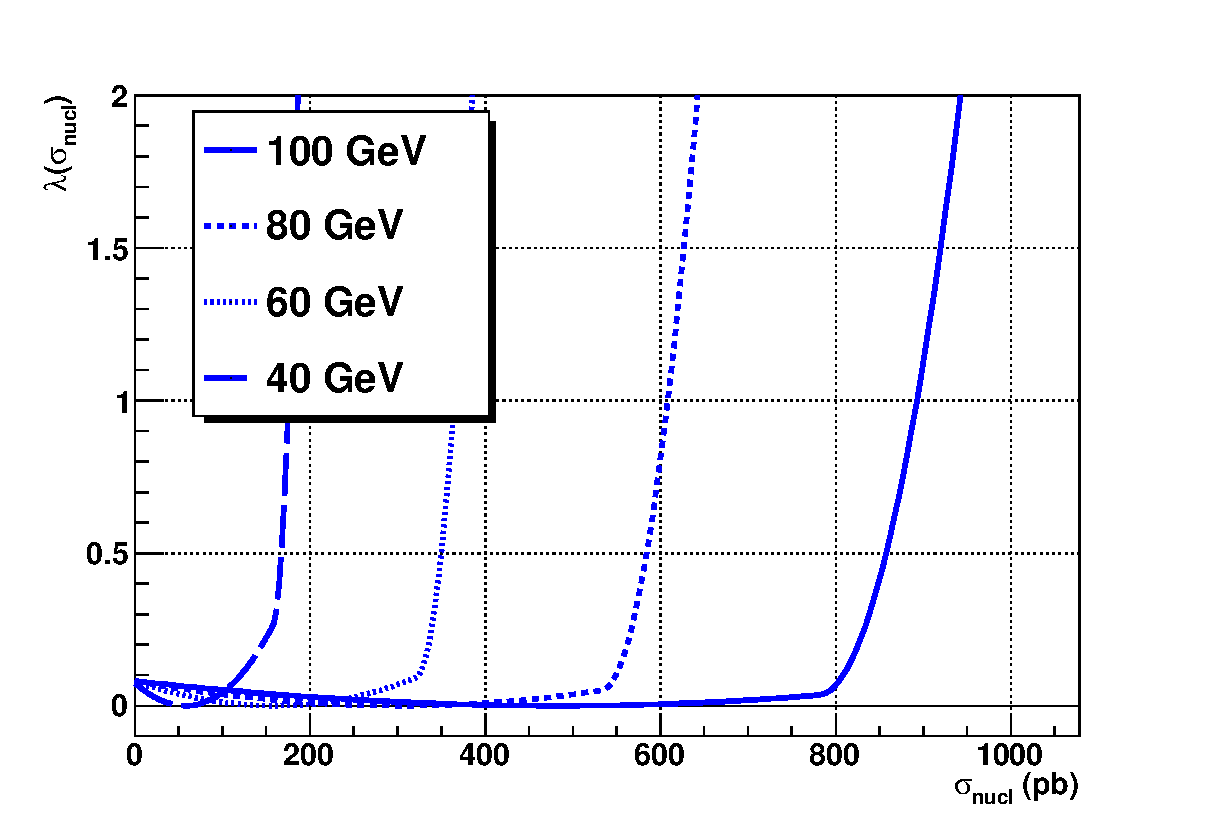
\includegraphics[height=0.4\textheight]{PLLCompare40.0}
				\label{fig:PLLRangeForty}
			}
			\subfigure[WIMP masses 4$\to$11~GeV]{
				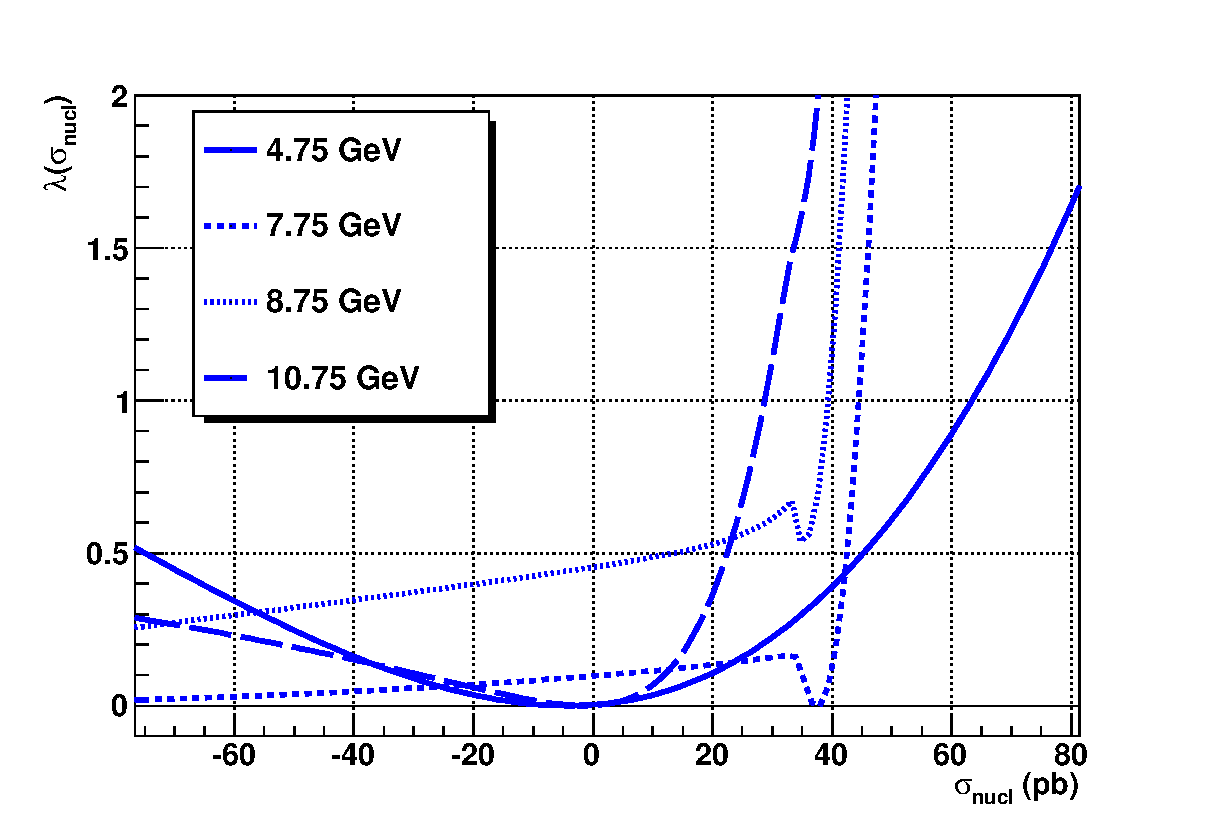
\includegraphics[height=0.4\textheight]{PLLCompare10.75}
				\label{fig:PLLRangeSeven}						
			}				
			\caption[$\pll$ for a range of WIMP Masses]
			{$\pll$ for a range of WIMP Masses.  See text for discussion of the shapes
			seen.}
			\label{fig:FitPathologies}
		\end{figure}
		
		\subsubsection{Signal, Background Similarity}
		\label{sec:LLPathoSBSimilarity}
			
			\begin{figure}
				\centering
				\includegraphics[width=0.9\textwidth]{WIMPModelCompare}
				\caption[Similarity of WIMP signal and background]
				{Similarity of signal and background, comparing the exponential and flat components of the background with a WIMP signal.  
				The shape parameter of the exponential function is set to -3.3 keV$^{-1}$, the best-fit value from data.  Flat and exponential backgrounds have 
				arbitrary normalizations for comparison to the WIMP signals.}
				\label{fig:SBSimilarity}
			\end{figure}			
			
			\begin{figure}
				\centering
				\subfigure[WIMP mass 100~GeV]{
					\includegraphics[height=0.4\textheight]{Summary100.0}
					\label{fig:SBCounts100}
				}
				\subfigure[WIMP mass 8.75~GeV, with zoom in on count region $0\to30$.]{
					\includegraphics[height=0.4\textheight]{Summary8.75}
					\label{fig:SBCounts8.75}						
				}				
				\caption[Counts in background components versus $\signuc$]
				{Counts in background components versus $\signuc$.  The values of the 
				components are determined during a profile-likelihood scan of $\signuc$.}
				\label{fig:SBCountsInComponents}
			\end{figure}	
		
For certain values of WIMP masses, the background and 	signal can appear very similar.  This can be seen, for example, in Figure~\ref{fig:SBSimilarity} which is a plot displaying WIMP signals of $M_{W}=8.75$ and 100~GeV together with an exponential spectrum ($e^{-3.3 E}$, the best-fit shape parameter for the model without included WIMP signal to data with a 99\% rise-time cut applied) and a flat spectrum both with arbitrary normalization adjusted for comparison.  Because $\pll$ includes an implicit maximization of the likelihood for different values of $\signuc$, it is instructive to consider how the components of those fits depend on $\signuc$.  Figure~\ref{fig:SBCountsInComponents} includes two plots of counts in background components (flat, exponential and L-line amplitudes) versus $\signuc$, where the background components are the parameters which maximize the likelihood for a given value of $\signuc$.  %These plots can help us understand features in the likelihood functions.  
If we first consider Figure~\ref{fig:SBCounts100} ($M_{W}$ = 100~GeV), it is clear that L-line background components vary only slightly with $\signuc$ whereas the exponential and flat components vary almost linearly with the flat component changing more quickly than than the exponential component.  When the limit of the flat background is reached at 0, it generates a kink in the likelihood function visible in Figure~\ref{fig:PLLRangeForty}.  Generally, parameters are allowed to float beyond their physically-allowed values to avoid such features in the likelihood function.  However, due to the similarity of the signal and background it was found that the flat background component would continue decreasing if it were allowed to float below zero leading to a very flat profile-likelihood function.  The linear variation of the flat and exponential background components with $\signuc$ coupled with the relative independence of the other parameter indicates that the variation of $\pll$ is dominated by the extended parameter\footnote{It can be shown that a minimization of this term leads to a linear dependence between the counts and $\signuc$.  If other terms in $\pll$ contribute, then the relationship becomes non-linear.}: $-\log \left( f_{Pois} \left( \sum_{x} N_{x}, N_{obs} \right) \right)$.  Therefore, the upper limit on $\signuc$ calculated using the profile-likelihood method is essentially equivalent to calculating a Poisson upper limit on true counts given number of counts seen, and assuming that all these counts come from signal.  %This equivalence gives confidence in this method.  

We can then consider lower WIMP mass (8.75~GeV) where the shape of the WIMP signal is roughly equivalent to the shape of the exponential background component in the data.  The relevant plots for this are Figure~\ref{fig:SBCounts8.75} and Figure~\ref{fig:PLLRangeSeven}, focusing on $M_{W}$=8.75~GeV in the latter.  It is important to note the $\pll$ for this mass does not intersect 0 in Figure~\ref{fig:PLLRangeSeven}; this is because no minimum of the $-\log L$ was found in the scanned region for $\signuc$ and was therefore defined as the value of $-\log L$ at the lowest scanned value of $\signuc$ (-100~pb).  To define an upper limit with this function, the Rolke prescription outlined in Section~\ref{sec:LimitsUnknownBackgroundML} would be followed, defining the minimum of $-\log L$ to be at $\signuc$ = 0.  It is clear that, in contrast to the previous case with signal of a WIMP at $M_{W}$=100~GeV, the flat and L-line components of the background are largely independent of $\signuc$, whereas the exponential component varies almost linearly below 35~pb and reaches its lower bound of 0 around 40~pb.  (The transition region between 35 and 40~pb which manifests a local minimum will be discussed in the following section.)  As before, the linear variation indicates that the likelihood is dominated by the extended term because the signal and background have a roughly equivalent shape.  The transition at higher $\signuc$ (50~pb) is due to the exponential shape constant floating to  $\sim0$ and taking over the contributions from the flat component.  This can be seen in Figure~\ref{fig:FitExpoShapeVsSigma}.
	
		\subsubsection{Local Minima of \texorpdfstring{$\pll$}{Profile-likelihood Function}}
		\label{sec:LLPathoLocalMinima}
			
			\begin{figure}
				\centering
				\includegraphics[width=0.9\textwidth]{ExpConst8.75}
				\caption[Exponential constant (shape parameter) versus $\signuc$]
				{Exponential constant (shape parameter) versus $\signuc$ for WIMP mass 8.5~GeV.
				The value of the exponential constant is determined during a profile-likelihood scan
				of $\signuc$.}
				\label{fig:FitExpoShapeVsSigma}
			\end{figure}
	
			\begin{figure}
				\centering
				\subfigure[$\signuc$ = 33.3~pb]{
					\includegraphics[height=0.36\textheight]{DataExclusionWIMPMass:8.75GeV33.3}
					\label{fig:ExpoFit33.3}
				}
				\subfigure[$\signuc$ = 34.8~pb]{
					\includegraphics[height=0.36\textheight]{DataExclusionWIMPMass:8.75GeV34.8}
					\label{fig:ExpoFit34.8}						
				}					
				\caption[Abrupt changed of exponential background shape during fitting]
				{Example of how the exponential background shape changes abruptly during a profile 
				likelihood scan for a WIMP Mass of 8.75~GeV.  The separate components of the fit are shown: 
				WIMP signal (dashed), L-capture lines (solid), exponential + flat background (dotted), and the 
				sum (solid). }
				\label{fig:FitExpoFitExample}
			\end{figure}	

The $\pll$ for $M_{W}$ = 8.75~GeV in Figure~\ref{fig:PLLRangeSeven} includes a local minimum contained in the range $34\leq\signuc\leq40$~pb.  From Figure~\ref{fig:SBCounts8.75}, it is clear this feature does not arise from the exponential background being at its limit since the amplitude does not reach its lower bound until $\signuc>$40~pb.  Instead, this characteristic is due to the fact that the exponential shape parameter is allowed to float to very negative numbers, producing a background function sharply decreasing with energy.  (The lower limits of this parameter were kept low enough so that no fit would push the parameter to its bound.)  This can be seen clearly in Figure~\ref{fig:FitExpoShapeVsSigma} where the exponential shape parameter decreases sharply around 30~pb after remaining largely constant for lower values of $\signuc$.  A complementary set of plots in Figure~\ref{fig:FitExpoFitExample} provide a visualization of this abrupt change.  This issue occurred when the shape of the exponential background was very similar to the shape of the applied WIMP signal which meant, for example, that the affected WIMP mass range was different for fits generated with data with rise-time cuts applied and for fits made on data with only microphonics cuts applied.  In particular, the rise-time-cut data exhibited a sharper exponential decline (more negative exponential shape constant) than the microphonics-cut data yielding an affected range of $\sim$6-9~Gev versus 7-10.5~GeV, respectively.  The abrupt variations in the exponential shape parameter also induced features in exclusion plots for $\sigman$; these are discussed in Sections~\ref{sec:LimitsUnbinned} and~\ref{sec:LimitsConstrained}.

		\subsubsection{Conclusions}
		\label{sec:LLPathoConclusions}

The realization of several non-parabolic features underscores the care which must be taken when deriving limits from models with similar background and signal.  Some methods (e.g.~the HESSE functionality in MINUIT~\cite{James:1975dr}) estimate the error on the parameter by assuming a parabolic shape and extrapolating $\pll$ around its minimum by using the measured second derivative at the extremum.  For non-parabolic $\pll$ functions it is clear this won't work, and could possibly yield inappropriate bounds on $\signuc$.  For example, in Figure~\ref{fig:PLLRangeSeven} the $\pll$ for $M_{W}$ = 7.75~GeV indicates a minimum at $\sim$37~pb: a parabolic estimate of the lower bound would be significantly non-zero 
whereas an estimate using the Rolke method would define the lower bound as 0!  Of course, as with all Frequentist methods it is essential to estimate the performance of the method using Monte Carlo tests; results of such an investigation are presented in Section~\ref{sec:LimitsCoverageTests}.

	\subsection{Coverage Tests}
	\label{sec:LimitsCoverageTests}			

		\begin{sidewaysfigure}
			\centering
			\subfigure[4.25$\to$8.25~GeV]{
				\includegraphics[width=0.46\textheight]{CoverageWithLastWIMP8.5}
				\label{fig:Coverage8.5}
			}
			\subfigure[8.5$\to$11~GeV]{
				\includegraphics[width=0.46\textheight]{CoverageWithLastWIMP13}
				\label{fig:Coverage13}						
			}
			\subfigure[13$\to$22~GeV]{
				\includegraphics[width=0.46\textheight]{CoverageWithLastWIMP50}
				\label{fig:Coverage50}						
			}												
			\subfigure[50$\to$100~GeV]{
				\includegraphics[width=0.46\textheight]{CoverageWithLastWIMP100}
				\label{fig:Coverage100}						
			}	
			% FixME JFW, why the different x axis ranges?				
			\caption[Coverage test results for WIMP mass range 4.25$\to$100~GeV]
			{Coverage test results for WIMP mass range 4.25$\to$100~GeV, see text for details. The range of the x axes ($\signuc$) differs since the coverage scans only
			cover values of the profile likelihood that satisfy $\pll \leq 2$.}
			\label{fig:CoverageTestResults}
		\end{sidewaysfigure}

Rolke et al.~emphasize that correct application of their method~\cite{Rol05} must be accompanied by a coverage test analyzing its effectiveness.  The protocol for this test is outlined in Section~\ref{sec:LimitsUnknownBackgroundML} where it is made clear that the \emph{entire} range of possible parameter space must be scanned.  For all but the most simple models, this is essentially impossible and so it is necessary to reduce the parameter space to a manageable size by selecting those parameter combinations which are the most `likely'.  Since we are primarily concerned with the coverage of the model versus the amount of included signal (proportional to $\signuc$), it is reasonable to use $\pll$ to define the considered parameter space.  $\pll$ provides a 1-dimensional path parameterized by $\signuc$ along an extremum in likelihood space, basically allowing the data to define which parameters of the model are the most likely.  It also reduces the scanned space to one dimension\footnote{In practice, the dimension is still 2 taking into account the variation of the WIMP mass.} thereby reducing the numerical problem to something tractable.  
To perform these tests, a model and a set of data were chosen to be the same as used throughout this section: the model used constrained the relative amplitudes of the Ge and Zn L-capture lines (see Section~\ref{sec:LimitsConstrained}) and the data used was that with a 99\% rise-time cut applied.  Each fit during this procedure was unbinned.  For each WIMP mass, a profile-likelihood function was calculated for $\signuc$ by calculating the maximum likelihood along a grid in $\signuc$-space.  At each point on this grid, the results of the fit (i.e.~parameter values maximizing $L$) were saved for later use.  Points were then selected from the $\pll$, first taking the best-fit result ($\pll = 0$) and then sampling the remainder of the space $\signuc > 0$ and $\pll \leq 2$ for 14 more points.  For each of these 15 points, 2400 toy simulations were run\footnote{For WIMP masses 5.5, 11, 70, and 100~GeV only 2000 toy simulations were run.  This was solely due to scheduling issues on the computer cluster used.} generating events according to the distributions defined by the parameters.  Since the models used an extended-likelihood formalism, the number of events generated for each simulation was Poisson distributed according to model parameters.  For each simulation, limits were calculated at 90\% confidence level using the Rolke technique.  The $\sim1$M simulations took roughly 1~year of 2.5~GHz CPU clock time, running on the Athena cluster at the University of Washington~\cite{Athena}.  

Results of these simulations are shown in Figure~\ref{fig:CoverageTestResults}, where the coverage is defined as the percentage of time the calculated limits included the `true' parameter value of $\signuc$, the value used to simulate the data set.  The results from the range of WIMP masses are split into four different plots and grouped together according to similar mass.  Each plot includes a line at 0.9, designating the expected coverage percentage as defined by the input confidence level.  These results indicate in general good coverage with under- and over-coverage mostly limited to within 5\% of the expected value.  The significant over-coverage for larger WIMP mass suggests that over the lower range values of $\signuc$, the signal is completely indistinguishable from background.  The coverage does tend back to 90\% at larger values of $\signuc$.  The under-coverage in Figure~\ref{fig:Coverage13} is likely due to the similarity of exponential background and WIMP signal and could also be affected by the profile-likelihood features discussed in Section~\ref{sec:LLPathologies}.  It is encouraging, however, that despite the fit difficulties and likelihood features discussed in Section~\ref{sec:LLPathologies}, the coverage remains close to 90\%.  This suggests that the Rolke method as applied to this model and data set is robust and that exclusions determined at 90\% confidence level are valid.

		\subsection{Limits from Unbinned and Binned ML Fits.}
		\label{sec:LimitsUnbinned}

Limits were calculated using data described in Chapter~\ref{chap:AnalysisBeGe} and the model in Section~\ref{sec:LimitsDataAndModel}.  The RooFit framework includes an abstracted interface for all data sets, making a transition between using a binned and unbinned analysis very simple and enabling a comparison between the two types of results.  Therefore, both binned and unbinned limits were calculated, selecting a bin size of 23.4~eV over the energy range (0.5$\to$3.5~keV, bin number: 128).  
Fits were performed for chosen values of $M_{W}$ in the range $3.75\to100$~GeV, sampling different ranges of the mass with a variable step size, $\Delta$: $3.75\to11$, $\Delta=0.25$~GeV; $11\to25$, $\Delta=1$~GeV, $30\to100$, $\Delta=10$~GeV.  Given the large amount of fits required to generate, the calculation method was parallelized for submission to the Athena cluster~\cite{Athena} at the University of Washington.  
			\subsubsection{Fit Components versus \texorpdfstring{$\signuc$}{sigma\_nuc}}
When running a large number of fits, it is challenging to provide effective quality control to ensure that the limit calculation has proceeded correctly.  To check this, the parameters of the values were tracked at their best-fit value (defined as the minimum $-\log L$ in the region $\signuc\geq0$) and at the 90\% exclusion limit of $\signuc$.  Examples of two of these plots are given in Figures~\ref{fig:UnbinnedResultsNoConstrain} and~\ref{fig:BinnedResultsNoConstrain} which are for unbinned and binned results, respectively.  The top three plots in each of these figures includes the individual components of the background events: the counts-per-kilogram-per-day in the exponential, flat, and separate L-line backgrounds.  The bottom plot includes the sum of the flat and exponential background and the sum of the Ge and Zn L-capture lines.  The parameters are generally smoothly varying versus $\signuc$ except in the region $\sim6\to10$~GeV where a significant amount of oscillation can be seen in the amplitudes of the flat and exponential components.  This oscillation is due mainly to the fact that the exponential shape constant is allowed to float positive and therefore can become indistinguishable from the flat background.  This is also confirmed by the largely-smooth behavior of the sum of the exponential and flat background components.  An example of the variation of the exponential shape parameter is discussed in Section~\ref{sec:LLPathologies} and shown in Figure~\ref{fig:FitExpoShapeVsSigma}.  However, some large variations do remain in the best-fit values of the sum components; these are due to the appearance in this WIMP mass region of local extrema away from the global minimum (see Figure~\ref{fig:PLLRangeSeven}).  Since the global extremum may be in the disallowed region (i.e.~$\signuc<0$), it is possible that the local minima are then interpreted as the global minima (i.e.~the best fit), but this is dependent on the granularity of the scanned $\signuc$ space and the size of the local minimum since it is possible to not sample fully the local minimum if it has a small width.  In other words, it is possible to `skip over' the local minimum and therefore interpret $\signuc=0$ as the best fit.  However, despite the sharp features in the best-fit values of the exponential and flat components it is clear that the value of the sum of these components at the 90\% exclusion of $\signuc$ varies smoothly.  

The amplitudes of each L-line component vary quite little versus $\signuc$.  Additionally, there is little to no difference between the amplitudes of these components at the global minimum and at the 90\% exclusion of $\signuc$.  This indicates that this portion of the background has little effect on the calculation of limits on a WIMP signal.

All of the same conclusions may be drawn from the binned analysis of the same data, results of which are shown in Figure~\ref{fig:BinnedResultsNoConstrain}.  As with the unbinned data, it is clear that some sharp features exist in the best fit of the sum of the flat and exponential components.  Regardless, the smoothness of the sum of the parameters at the 90\% exclusion of $\signuc$ implies that any sharp variation in the best-fit parameters are irrelevant.  The similarity between binned and unbinned results indicates the robustness of the maximum-likelihood technique and also suggests that an unbinned analysis could be unnecessary for data with this number of counts.
  
			\begin{figure}
				\centering				
				\includegraphics[width=0.85\textwidth]{unconstrained_unbinnedresults_rt_95AllComponentsLN+microphonicscuts,Rise-timecut:95}				
				
				\caption[Fit results using unbinned data with 95\% rise-time cut (+ microphonics cut) applied]
				{Results from an unbinned fit using data with 95\% rise-time cut (+ microphonics cut) applied.
				The top three figures contain the variation of all independent parameters at their best-fit value and at the 90\% exclusion
				limit of $\signuc$.  The bottom figure contains a sum of the background components (flat + exponential) and
				the L-lines.  See text for details.  Lines between points are included to guide the eye.}
				\label{fig:UnbinnedResultsNoConstrain}
			\end{figure}
			\begin{figure}
				\centering				
				\includegraphics[width=0.95\textwidth]{unconstrained_binnedresults_rt_95AllComponentsLN+microphonicscuts,Rise-timecut:95}				
				
				\caption[Fit results using binned data with 95\% rise-time cut (+ microphonics cut) applied]
				{As Figure~\ref{fig:UnbinnedResultsNoConstrain} but with binned data.}
				\label{fig:BinnedResultsNoConstrain}
			\end{figure}
			
			\begin{sidewaysfigure}
				\centering
				\subfigure[Unbinned]{
					\includegraphics[width=0.46\textheight]{unconstrained_unbinnedall_exclusion_plots80}
					\includegraphics[width=0.46\textheight]{unconstrained_unbinnedall_exclusion_p1000}
					\label{fig:UnconstrainedLimitsUnbinned}						
					
				}												
				\subfigure[Binned]{
					\includegraphics[width=0.46\textheight]{unconstrained_binnedall_exclusion_plots80}
					\includegraphics[width=0.46\textheight]{unconstrained_binnedall_exclusion_p1000}				
					\label{fig:UnconstrainedLimitsBinned}						
				}
				\caption[90\% CL limits on $\sigman$ for various data sets]
				{90\% CL limits on $\sigman$ for various data sets.}
				\label{fig:UnconstrainedLimits}
			\end{sidewaysfigure}			
			
			\subsubsection{Exclusion Limits}	
Exclusion limits at 90\% confidence level for $\sigman$ are shown in Figure~\ref{fig:UnconstrainedLimits}, with $\sigman$ calculated from $\signuc$ given the relationship in Equation~\ref{eqn:SigmaConversion}.  Results for both binned and unbinned data are split into two plots each to allow clearer visualization of exclusions calculated for data sets with different cuts applied.  
It is clear that there exists very little distinction between limits on binned and unbinned data; however, several features are apparent among the different data sets.  In the low-WIMP-mass range, 4-5.5~GeV, all the curves are very similar suggesting the limits in this small region are robust against cuts to the data.  At higher WIMP mass, 20-100~GeV, the slope of the curves is very similar, though the normalizations are somewhat different.  As expected, in this region the microphonics-cut data exhibits more conservative limits than the rise-time cut-data.  The variation in the limits calculated from rise-time-cut data is expected to arise from systematic errors on the estimation of the efficiencies of these cuts as well as from the unknown ratio, (signal)/(signal + background), for each cut.  

The mass range 6-9~GeV exhibits sharp features in the exclusion plots, existing in WIMP-mass regions where the shape of the signal is very similar assumed to the shape of the background.  These features also appear in the microphonics-cut data, but at a slightly higher mass range from $\sim7\to10.5$~GeV.  These characteristics are essentially an indication that the calculated exclusion limit comes when the amplitude of the WIMP signal completely takes over the contribution from the exponential fit component.  An example of this is given in Figure~\ref{fig:WIMPFitExampleSigLikeBgd} which displays the fit at the 90\% CL exclusion of $\sigman$.  It is clear that at this value of $\sigman$, the WIMP signal fits to the low-energy data without any contribution from the exponential background.  Close inspection also reveals that the exponential shape parameter has transitioned to a positive value, resulting in a mildly increasing background with energy.  

			\begin{figure}
				\centering
				\includegraphics[width=0.9\textwidth]{WIMPMass8GeVFinalFit}
				\caption[Signal exclusion fit at 90\% CL.]
				{Fit at 90\% CL exclusion, $\sigman = 1.2 \times 10^{-4}$~pb.  
				WIMP signal is blue dashed, L-lines in solid red, flat + exponential background in dotted red, and 
				sum of all the pdfs is blue solid.
				This is an unbinned fit with 95\% rise-time cut data.  }
				\label{fig:WIMPFitExampleSigLikeBgd}
			\end{figure}

At low-mass range the microphonics-cut data demonstrates a stronger limit than the 80\%$\to$99\% rise-time-cut data.  Initially this seems counter-intuitive, but can be explained due to the fact that the microphonics-cut data includes a larger contamination of slow-rise-time pulses which is not well fit with a single exponential.  This indicates that the background distribution coming from slow rise-time pulses is not properly included in the set of background pdfs.  Since this distribution is not known a-priori, the proper inclusion would require a source measurement to estimate its shape.  It is interesting to note that the exclusion calculated using 99\% rise-time cut data demonstrates a transition between the microphonics cut data and the 95\% rise-time cut data around 6~GeV.  The shape and coverage of the rest of the rise-time cut exclusions are similar, suggesting that the rise-time cut retains a consistent shape in the data as the acceptance is decreased from 99\%.  It also implies that some slow-rise-time-pulse background remains at 99\% acceptance, consistent with results from Section~\ref{sec:RisetimeSystematicTests} which demonstrated a slightly less-negative exponential constant with the 99\% rise-time-cut data as compared to rise-time cuts with less acceptance.  This final conclusion indicates that data with at least a 95\% rise-time cut should be used to generate exclusions since these data will have as little slow-rise-time-pulse contamination as possible.  

		\subsection{Constrained Ge and Zn Relative Amplitudes}
		\label{sec:LimitsConstrained}
	
The relative amplitudes of the Zn and Ge L-capture lines may be constrained by
the K-capture lines of the same isotopes since the K- to L-capture ratio has
been well understood through independent
measurements~\cite{Schonfeld1994955,Ocampo1962}, see Table~\ref{tab:LKRatios}.
The amplitudes (in counts) of the Ge and Zn K-lines were measured using an
unbinned fit of the 99\% rise-time-cut data\footnote{The 2~month live-time data
was used to calculate this ratio.} and determined to be 945.1$\pm28.2$ and
349.7$\pm19.1$, respectively\footnote{This measurement was performed using a
smaller subset of data with 2~months of live-time.}.  Therefore, the expected
ratio of the Ge and Zn lines (Zn/Ge) was 0.33$\pm$0.02.  The relative
amplitudes of these lines in the fitting model were then constrained by this
value, reducing the number of parameters in the fit by one.  In general, it
would be more desirable to tie this ratio to the amplitudes of the K-capture
lines and perform a simultaneous fit, but since the relative amplitudes of the
lines did not vary significantly when allowed to float independently and since
the measurements of each set of lines were in separate channels (high-,
low-gain channels for L-,K-lines, respectively), it was not expected that
proceeding in such a manner should have a significant impact.  Final results of
the fit supported this initial assumption.
	
			\begin{table}
				\centering
				\caption[L/K capture ratios for \gersixeight~and \znsixfive]
				{L/K capture ratios for \gersixeight~and \znsixfive.  The theory of Brysk and Rose~\cite{Bry58}
				has corrections applied via Bahcall~\cite{Bah63}.  
				Useful tabulations for calculating L/K values are found in~\cite{Wap59}.}
				\label{tab:LKRatios}
				\begin{tabular}{lcr}
					\toprule
					Atom & Value & Ref.\\
					\midrule
					\gersixeight & 0.1328$\pm$0.002 & \cite{Schonfeld1994955}\\
					\znsixfive & 0.119$\pm$0.007 & \cite{Ocampo1962}\\
					\gersixeight~(theory, corrected) & 0.126 & \cite{Bry58,Bah63} \\
					\znsixfive~(theory, corrected) & 0.108 & \cite{Bry58,Bah63} \\
					\bottomrule
				\end{tabular}	
			\end{table}
			
			\begin{figure}
				\centering				
				\includegraphics[width=0.95\textwidth]{constrained_unbinnedresults_rt_95AllComponentsLN+microphonicscuts,Rise-timecut:95}				
				\caption[Unbinned fit results, constraints on relative amplitude of Ge and Zn lines]
				{As Figure~\ref{fig:UnbinnedResultsNoConstrain}, but with a constraint on the relative amplitudes 
				of the Ge and Zn lines.  Therefore, only the sum of the L-lines (and not each contribution) is included.  }
				\label{fig:UnBinnedResultsConstrain}
			\end{figure}
					
			\begin{figure}
				\centering				
				\includegraphics[width=0.95\textwidth]{constrained_binnedresults_rt_95AllComponentsLN+microphonicscuts,Rise-timecut:95}
								
				\caption[Binned fit results, constraints on relative amplitude of Ge and Zn lines]
				{As Figure~\ref{fig:UnBinnedResultsConstrain}, but with binned data.}
				\label{fig:BinnedResultsConstrain}
			\end{figure}
			
			\begin{sidewaysfigure}
				\centering
				\subfigure[Unbinned]{
					\includegraphics[width=0.46\textheight]{constrained_unbinnedall_exclusion_plots80}
					\includegraphics[width=0.46\textheight]{constrained_unbinnedall_exclusion_p1000}			
					\label{fig:ConstrainedLimitsUnbinned}						
				}												
				\subfigure[Binned]{
					\includegraphics[width=0.46\textheight]{constrained_binnedall_exclusion_plots80}
					\includegraphics[width=0.46\textheight]{constrained_binnedall_exclusion_p1000}			
					\label{fig:ConstrainedLimitsBinned}						
				}
				\caption[Limits on $\sigman$ constraining the relative amplitudes of Ge and Zn L-lines]
				{Limits on $\sigman$ constraining the relative amplitudes of Ge and Zn L-lines.}
				\label{fig:ConstrainedLimits}
			\end{sidewaysfigure}		
			
Results are presented as in Section~\ref{sec:LimitsUnbinned}, with a representative set of plots of parameters versus WIMP mass (Figures~\ref{fig:UnBinnedResultsConstrain},~\ref{fig:BinnedResultsConstrain}) and exclusion limits in Figure~\ref{fig:ConstrainedLimits}.  As before, it was determined that very few differences manifested between the binned and unbinned results.  The amplitude of the sum of the L-lines appears very similar ($\sim6$~Counts/kg/d) as with the unconstrained fit (Figure~\ref{fig:UnbinnedResultsNoConstrain}).  However, this comes as little surprise given the relative independence and lack of variation of these parameters in the unconstrained fits.  Because of the clear similarity between the constrained and unconstrained results, the conclusions regarding this set are equivalent to the previous.  However, the results of this section further emphasize that the amplitudes of the L-lines have little effect on the exclusion of a low-mass-WIMP signal since the sum of the L-lines varies so minimally with WIMP mass.  Also, little difference exists between the amplitude of the L-line at best fit and at 90\% exclusion, indicating that these parameters have very little sensitivity to $\signuc$.

	\section{Conclusions and Discussion}
	\label{sec:LowMassWIMPConclusions}


		\begin{figure}
			\centering
			\includegraphics[width=0.9\textwidth]{MGM_Thesis_Compare_plot}
			\caption[Comparison of exclusions to CDMS, DAMA, and previous CoGeNT results.]
			{Comparison of results from this analysis to other results.  Included lines are 90\% CL 
			exclusion limits using 95\% (black dashed) and 70\% (black solid) rise-time-cut data sets, 
			results from the previous CoGeNT detector~\cite{Aalseth:2008aa} (red dotted), 
			most recent CDMS results~\cite{Ahmed:2009zw} (gray solid), and acceptance regions
			from DAMA data as interpreted in~\cite{Savage:2008er} ($3\sigma$ dark green region,
			$5\sigma$ light green region).  Plot generated with dmtools.brown.edu~\cite{Gai03}.}
			\label{fig:BeGeLimitsComparedToOtherDataSets}
		\end{figure}		

The data from the modified-\bege~detector deployed underground at Soudan Underground Laboratory have been used to generate limits on spin-independent WIMP interaction cross-section.  A framework has been developed that should prove useful in generating limits using other R\&D detectors and the \MJ~\minmod.  The results of the data from this detector may be compared to other experimental results as well.  For example, in Figure~\ref{fig:BeGeLimitsComparedToOtherDataSets}, limits from these results are compared to previous results with a similar detector from CoGeNT~\cite{Aalseth:2008aa}, the most recent published data from the CDMS collaboration~\cite{Ahmed:2009zw}, and regions of acceptance for the DAMA data as interpreted in~\cite{Savage:2008er}.  

The DAMA experiment is a NaI-based experiment that has observed an annual
modulation in their data.  Interpreting this feature in their data as
interactions of low-mass WIMPs yields the acceptance regions presented in
Figure~\ref{fig:BeGeLimitsComparedToOtherDataSets}.  The germanium-based CDMS
experiment has the ability to distinguish between electron and nuclear recoils,
enabling it to achieve far lower bounds on $\sigman$.  However, the threshold
of the CDMS detectors limits their sensitivities to WIMP masses above
$\sim7$~GeV.  It is clear that results from this analysis fully exclude the
DAMA $3\sigma$ acceptance region at low WIMP mass and remove almost all of the
allowed space of the $5\sigma$ region save some space at mass below
$M_{W}=4$~GeV and some mass regions from $6\to10$~GeV.  Accessing the region at
low mass will require a further reduction of threshold below 0.3~keV. 
%FixME, put in a WIMP plot here to demonstrate this?
The exclusion of the still-accessible $5\sigma$ region $6\to10$~GeV will demand
a clearer understanding of the unknown exponential background since the
similarity between this background and a WIMP signal forces the limits high in
this region.  Rejecting this background as a possible WIMP signal can also come
from looking at the time behavior of the data to see if it exhibits any annual
oscillation characteristic of moving through the WIMP halo.  The
\MJ~\minmod~will have an enhanced sensitivity to a rate modulation given its
larger mass and exposure time.  The physics reach of the \MJ~\minmod~and 
additional analyses related to other dark matter candidates will be 
explored in the following chapter.



%Things to discuss:
%Also, expect to apply the methods to R\&D detectors around the collaboration.
%Outlined a generic WIMP signal for application in 2-D time and energy space.

%Outlined and explored a methodology for generating limits in the presence of unknown background. 

%Explored the coverage of this methodology, found that it behaved well even given the difficulties found.

%Performed the fits, performed systematic tests, found robust against modification of binned, and un-binned results, constraining L-capture lines

%Apply these data to other data sets, in particular compare to the results of other experiments (DAMA, CDMS, etc.)
%In the context of Majorana, a set of tools and a procedure was developed for generating dark matter limits.  In particular, given the small data rate expected from the \minmod~and the large detector mass, we expect to be able to apply these results and methods to MJ.  
 
\clearpage


% ========== Chapter 6
 
\chapter{Other low-energy physics with P-type point contact detectors}

%In this section, we basically discuss two things: Heavy non-relativistic axions, the signal, and the exclusion limit as calculated with the data from the previous chapter.
	
%Also, making some reasonable assumptions about Majorana, we make some estimates as to the sensitivity of the Majorana experiment to WIMP dark matter and axion dark matter (via the axioelectric effect).  

	The high resolution and low threshold of p-type point-contact detectors makes them sensitive to other dark matter signals in addition to those from WIMPs.  This chapter explores this, deriving limits on the inelastic scattering of pseudoscalar dark matter candidates off of electrons.  The \MJ~\minmod~will deploy an array of \ppc~detectors with a significantly lower background ($\gtrsim10^{3}$ reduction in count rate) than seen in the data set presented in this thesis.  The latter half of the chapter estimates the sensitivity the \MJ~experiment to dark matter candidates making some conservative assumptions on the shape and magnitude of the expected background.  
		
	\section{Other dark matter candidates: keV-scale bosons}
	\label{sec:CalcLimitsOnHeavyAxions}		

	The lack of understanding as to how a dark matter particle couples with normal `Standard Model' matter has motivated wide theoretical investigation resulting in candidate particles in addition to WIMPs.  As well, results from the NaI-based DAMA experiment~\cite{Bernabei:2005ca} have demonstrated a clear annual modulation signal which could be interpreted as arising from the earth's movement through a galactic cloud of dark-matter particles.  Because other experiments sensitive to WIMP interactions have failed to reproduce this result, the possibility remains that some non-WIMP-like process could underly the cause.  However, the results of the DAMA experiment are not the sole motivation for studying dark matter candidates beyond WIMPs.  Whereas most dark matter experiments focus their sensitivity on looking for one type of signal (i.e.~a nuclear recoil from a WIMP interaction), it is still essential to consider other possibilities.  
	
	Pospelov et al.~have completed a study~\cite{Pospelov:2008jk} analyzing the possibility of keV-mass bosons as dark matter candidates.  In particular, they outline the expected interactions and rates for scalar, pseudoscalar, and vector bosons incident upon modern detectors.  In general, Pospelov et al.~avoid in-depth discussions regarding theoretical motivation of each bosonic type, but the mathematics behind the pseudoscalar are the same as that for an axion, the particle responsible for preserving CP in QCD (see, e.g.~\cite{Amsler20081}).  Because of this equivalence, other work deriving axion processes or limits on such processes remains relevant in this case.  The following sections consider the coupling of a pseudoscalar to electrons in a detector and therefore refer to this process as an `axioelectric' effect and the originating particle as an `axion.'  

	\subsection{Axioelectric signal}
	\label{sec:CalcLimitsOnHeavyAxionSignal}		

	The signal for a non-relativistic axion interacting via the axioelectric effect has been derived in~\cite{Pospelov:2008jk}.  This particular inelastic interaction involves the deposition of the \emph{complete} energy of the axion, which in the non-relativistic case is essentially equal to the mass of the particle.  Since the excitation of the electron via the axioelectric effect is similar to the process mediated by a photon in the photoelectric effect, the signal is a delta function centered at the mass of the axion, $m_{a}$.  Convolved with the detector resolution, the signal would appear gaussian with width exactly that of a gamma or x-ray of energy equivalent to $m_{a}$.  The rate of this interaction has been estimated in~\cite{Pospelov:2008jk} as:
	
		\begin{equation}
			R \left[ \text{kg}^{-1} \text{day}^{-1} \right]\simeq \frac{1.2\times 10^{19}}{A} \gaa^{2} m_a \sigma_{photo}
			\label{eqn:AxioelectricRate}
		\end{equation}

where $A$ is the atomic mass, $m_{a}$ is the mass of the axion in keV, $\sigma_{photo}$ is the measured photoelectric cross section in barns, and $\gaa$ is the dimensionless coupling constant related to the normal axion coupling constant $f_{a}$ by $\gaa \equiv 2 m_{e}/ f_{a}$ ($m_{e}$ is the mass of the electron).  In the derivation of this result, the value of the density of dark matter was used: $\rho_{D}$ = 0.3~GeV~cm$^{-3}$.  Also, Pospelov et al.~noted that this interaction rate should not exhibit a significant annual modulation from the earth's orbital velocity and therefore no time dependence was included in the equation.  The rate calculated for a germanium detector ($A=72.96$) with a chosen coupling constant, $\gaa = 10^{-11}$, is shown in Figure~\ref{fig:HeavyAxionSignalRate}.  The rate calculation used well-known cross sections obtained from the NIST FFAST database located online~\cite{chantler:597}.  The sharp feature in the plot around $m_{a}\sim1.3$~keV arises from the L-line resonance at this energy.  Other sharp features similarly relate to the energy levels of electrons in a germanium atom.  

The low noise of \ppc~detectors yields excellent sensitivity to non-relativistic axions with masses $\leq10$~keV due their sharp resolution at low energies.  This enhanced performance is especially clear when considering the capabilities of NaI detectors used in the DAMA experiment.  A comparison of an axioelectric signal at a given $\gaa$ is provided in Figure~\ref{fig:ResCompare} for characteristic resolutions of NaI and germanium detectors.  In this plot, it is clear that the improved resolution of the germanium detector allows less smearing of the signal, forcing more counts into a narrower peak.  The enhanced resolution enables superior distinction of the signal in the presence of background.

		\begin{figure}
			\centering
			\includegraphics[width=0.9\textwidth]{GeRate}
			\caption[Axioelectric interaction rate in germanium]{Non-relativistic axion axioelectric 
			interaction rate in germanium.  The photoelectric cross section for germanium was obtain
			from the NIST database~\cite{chantler:597}.}
			\label{fig:HeavyAxionSignalRate}
		\end{figure}

		\begin{figure}
			\centering
			\includegraphics[width=0.9\textwidth]{DAMARes}
			\caption[Axion signal at $m_{a}$ = 3.2~keV]{Axion signal at $m_{a}$ = 3.2~keV comparing 
			the detector responses of germanium (blue, dashed) and NaI (red, solid) to an equivalent
			$\gaa$.  }
			\label{fig:ResCompare}
		\end{figure}

	\subsection{Limits on the axioelectric effect}
	\label{sec:CalcLimitsOnHeavyAxionLimits}		
		
	Limits were calculated using the profile-likelihood method described in Section~\ref{sec:LimitsML}.  Fits were performed on the complete number of data sets described in Chapter~\ref{chap:AnalysisBeGe}, with a total live-time of 150.6~days.  All data sets yielded similar results and so one data set was chosen with 95\% rise-time acceptance cuts and microphonics cuts applied.  As outlined before, assumptions about the source of slow-rise-time events reduced the fiducial mass to 0.33~kg (see Section~\ref{sec:BeGeLowEnergyFeatures}).  Additionally, results with unbinned and binned maximum-likelihood fits were consistent and so the former was used for the final result.  The limit calculation followed the same procedure as a peak search in the data and is outlined as follows:
		\begin{itemize}
			\item Define the gaussian signal $f_{axion}$: 
			\begin{itemize}
				\item Choose mass $m_{a}$ of the axion defining $\mu$ of gaussian
				\item Determine $\sigma$ at $E = m_{a}$ using resolution in Equation~\ref{eqn:SigmaEqn}.
			\end{itemize}
			\item Fit to the function $B + N_{axion} f_{axion}$ where $B$ is the background defined in Section~\ref{sec:LimitsDataAndModel} and determine the profile likelihood $\plln$.
			\item Determine the 90\% upper limit on $N_{axion}$ using $\plln$.
			\item Repeat for other values of $m_{a}$
		\end{itemize}		
	
	During the fits, the $\mu$ and $\sigma$ of the gaussian signal, $f_{axion}$, were kept fixed and only the amplitude, $N_{axion}$ was kept as a free parameter of the signal.  For the background, the behavior of the parameters was the same as during WIMP exclusion fits (see Section~\ref{sec:LimitsDataAndModel}) and the relative amplitude of the \gersixeight~and \znsixfive~L-lines was kept fixed as described in Section~\ref{sec:LimitsConstrained}.  Fixing this relative amplitude served to minimize the impact of the L-lines in the exclusion fits since a signal centered at 1.1 or 1.3~keV would look exactly like either L-capture line.  The difficulties seen while determining limits on low-mass WIMPs did not appear in these calculations because the signal (gaussian centered at $m_{a}$) was not similar to the background except for the case of the L-lines.  The value of the axion mass was scanned from 0.1~keV to 7.8~keV in steps of 0.2~keV using both high- and low-gain channels: high-gain channel, $0.1\to2.9$~keV; low-gain channel, $3\to7.8$~keV.  The axion mass was allowed to vary below threshold (0.5~keV) because the finite resolution of the detector would allow portions of the expected gaussian signal to be detected above threshold.  An example of an exclusion fit in the high-gain channel is shown in Figure~\ref{fig:ExampleHeavyAxionFit} for $m_{a}=3$~keV.  

		\begin{figure}
			\centering
			\includegraphics[width=0.9\textwidth]{AxioelectricFitExample}
			\caption[Example of an excluded non-relativistic axioelectric signal at $m_{a}=3$~keV at 
			90\% CL]{Example of an excluded non-relativistic axioelectric signal at $m_{a}=3$~keV at 
			90\% CL.  In this fit performed in the high-gain channel, the excluded value $N_{axion}$ 
			is 36.1 counts.  
			The components of the fits are split: red solid, L-Lines; red dotted, flat plus exponential
			background; blue dashed, excluded axioelectric signal.}
			\label{fig:ExampleHeavyAxionFit}
		\end{figure}
			
	The 90\% CL excluded rate in counts/kg/day, $R_{axion}(m_{a})$, was determined from $N_{axion}$
and from this value the upper limit of $\gaa$ could be determined.  The exclusion calculated from this result is presented in Figure~\ref{fig:HeavyAxionLimits} 
along with a comparison to other results, including previous results of the CoGeNT collaboration~\cite{Aalseth:2008aa}, the CDMS 
collaboration~\cite{Ahmed2009}, and an acceptance region from the DAMA collaboration~\cite{Bernabei:2005ca}.  As noted in both 
references~\cite{Collar:2009sp,Pospelov:2008jk}, the limit calculation performed in~\cite{Bernabei:2005ca} did not correctly treat the 
leading term in the Hamiltonian, producing instead a reduced rate around 3 orders of magnitude lower for a given $\gaa$.  An estimation 
of the corrected result from DAMA as outlined in~\cite{Collar:2009sp} appears in Figure~\ref{fig:HeavyAxionLimits}.  A comparison to 
limits derived from both solar neutrinos~\cite{Gondolo09} and globular clusters~\cite{Raffelt95} is included as well.  

The strongest limits obtained from astronomical observation arise from determining how much `hidden energy' may be carried off by axions from the solar 
core (in the case of solar neutrinos) and similarly from the cooling observed in the evolution of red-giant stars in globular clusters.  All 
direct measurements provide stronger limits than those from solar neutrinos, but the mass-independent limits from globular-cluster 
stars still exceed all others.  Supernovae generally provide the best constraints on axions and other exotic particles, but their high temperatures ($O$(10~MeV)) mean that axion-electron interactions are suppressed according to $m_{e}^{2}/T^{2}$~\cite{Pospelov:2008jk}.  Other limits on pseudoscalars from cosmological observations are possible, including searches for decays to photons and estimates of axion abundance from the big bang.  These limits are discussed with respect to the sensitivity of the \MJ~\minmod~in Section~\ref{sec:MJSensitivityToAxions}.  Even though the presented direct-detection limits are already well within the space disallowed by astronomical constraints, it is still important to explore these parameter regions since limits from both cosmological observation and experiment can depend strongly on choices of models and their parameters.
			
	Pospelov et al.~noted the axioelectric process should be to first order invariant to the velocity of the incoming dark matter particle and so would not generate an appreciable annual modulation.  This would limit any interpretation of the DAMA annual modulation as due to an axioelectric interaction and would therefore disallow the DAMA acceptance region in Figure~\ref{fig:HeavyAxionLimits}.  Collar et al.~point out the possibility of recovering the annual modulation effect by considering the axioelectric interaction rate as not arising from changes in incident dark matter velocity but rather from the annual variation of the number density of the particles~\cite{Collar:2009sp}. 
			
		\begin{figure}
			\centering
			\includegraphics[width=0.9\textwidth]{axion_constrained_unbinnedall_exclusion_plots_final}
			\caption[Limits on the axioelectric coupling constant $\gaa$]{Limits on the axioelectric 
			coupling constant $\gaa$.  Results from this work appear in comparison to previous 
			results from CoGeNT~\cite{Aalseth:2008aa}, CDMS~\cite{Ahmed2009}, and 
			DAMA~\cite{Bernabei:2005ca}.  The DAMA results have been corrected per 
			reference~\cite{Collar:2009sp}.  Limits derived from both solar neutrinos~\cite{Gondolo09} and globular clusters~\cite{Raffelt95} are included as noted, see text for details.}
			\label{fig:HeavyAxionLimits}
		\end{figure}
		
	\subsection{Conclusions and Discussion}
	\label{sec:DiscOnHeavyAxionLimits}	

%	Note what we've done here, in particular looking at an axioelectric signal in data.  Also note that this is one very small detector that's comparable to a large array.  Talk about how this could be better with MJ and how the limits from astrophysical observations still need to be checked.  
	
	The results from this section underscore and emphasize the physics reach of \ppc~detectors.  In particular, a limited amount of data from a small `table-top' detector (mass exposure $\sim50$~kg-days) yielded results comparable to and in some cases better than results from CDMS which had more than a factor of 5 greater exposure time (443.2~kg-days).  Though limits derived from astronomical observations still exceed those from direct-detection experiments, it remains important to verify these limits and, if possible, better them with larger exposure times and smaller backgrounds.  The need to explore dark matter candidates beyond those offered by WIMP theories remains evident and the only method to ensure experimental sensitivity to rare events with an \emph{a priori} unknown signature is to reduce known backgrounds through appropriate shielding and detector component radio-purity.  The \MJ~experiment seeks to do this to search for $\nonubb$, but the same efforts to reduce backgrounds in the double-beta decay signal region ($\sim2$~MeV) should benefit searches for dark matter in low-energy regions.  The following sections discuss and calculate the sensitivity of the \MJ~\minmod~for such searches.
							
	\section{Sensitivity of the \MJ~\minmod~to dark matter signals}
	\label{sec:MJSensitivity}
	
	Since a framework was established to determine exclusion limits for low-mass WIMPs and for the axioelectric coupling constant, it is simple to apply this same framework to determine the sensitivities of the \MJ~\minmod~to these two dark matter signals.  The ultra-clean composition of the \minmod~should provide an excellent detector for searching for dark matter without relying upon significant background reduction cuts (e.g.~discrimination between nuclear and electron recoils).  Calculating the sensitivity of the experiment involves making some assumptions of the background at low energies and of the makeup of the experiment.  A discussion about the estimation of the background follows in Section~\ref{sec:MJLowEnergyBackgroundModel}.  The general prescription for calculating the sensitivity is outlined:
	
		\begin{itemize}
			\item Generate a background model, including an expected rate of background
			\item Simulate a spectrum according to the background model
			\item Fit to the simulated spectrum the background model plus a signal model (e.g.~WIMP or axioelectric spectrum)
			\item Calculate the upper limit on the amplitude of the signal at 90\% CL.
			\item Repeat a large number of times ($O$(1000)) to generate an ensemble of limits.
		\end{itemize}	
		
The generated ensemble of limits for a particular signal would create a distribution of limits.  The 90\% CL limit was chosen as the limit which was above 99\% of the entries in this distribution.  Details of the \MJ~\minmod~are given in Section~\ref{sec:MJExperiment}, but for these purposes we have conservatively assumed that the \MJ~\minmod~will be composed of 20~kg of material and that it will run to accumulate between 1 and 5~years of live-time.  
	
		\subsection{Low-energy background model}
		\label{sec:MJLowEnergyBackgroundModel}
		
The estimation of background generally comes from verified simulations and from extrapolations from previous experiments.  In this work, the background is estimated by assuming it arises from two main sources: (1) a continuum from higher energy processes, and (2) counts from the beta decay of cosmogenically-produced tritium in the detector.  A simulation to estimate (1) is wrought with challenge since a large number of contributions can affect the result.  However, it is possible to use previous results from low-background germanium-based experiments to produce an estimate of this background.  The IGEX experiment measured a flat background rate of $\sim0.1$~counts/keV/kg/day in this low energy region ($4\to10$~keV)~\cite{Ira01}.    The \MJ~\minmod~plans to reduce background above 200~keV by a factor of 100~\cite{Gaitskell:2003zr} and so it is reasonable to expect the flat background at low energies will follow this same reduction to be roughly 0.001~counts/keV/kg/day.  This background was assumed stable in time as well, so that it was flat in both time and energy.

The estimate of a background to tritium involves understanding the activation rate of tritium for germanium at the surface of the earth.  This activation rate has been estimated to be $\lesssim200$~\hthree-atoms-per-kilogram-of-Ge-per-day for natural germanium at the surface of the earth, and almost a factor of 2 less for germanium with enriched \gersevensix~content~\cite{Avi92}.  The exposure is determined by the time of manufacture beginning with the pulling of the germanium crystal since the tritium content is `reset' at this point.  For example, if the entire process from crystal pulling to detector development and then final deployment (or storage) underground takes 15~days, then this integrated time is the the total tritium activation period for the detector.  For a kilogram natural-germanium detector created over such a time scale, we would expect there to be $15\times200\sim3000$ atoms of \hthree~within the detector.  Given the slow time of decay of \hthree~(12.32~years), it is critical to minimize the time above ground and certainly necessary to avoid any time at high altitudes, e.g.~storage or transport via airplane.  In this simple background model, two optimistic exposure times are chosen -- 15 and 30~days -- and it is assumed that the detectors begin taking data immediately after arriving underground.  In practice, the assumption of immediate detector commissioning is justified due to the long decay time of tritium: the detector will not significantly cool down during a period of time underground much shorter than the lifetime.  The average rates due to these exposures once underground are then roughly 0.03 and 0.06~counts/keV/kg/day for 15 and 30~days, respectively.  

The pdf of the tritium decay function was constructed in both time and energy using the uncorrected kinematic equation:
		\begin{equation}
			f_{^{3}\text{H}}\left(E, t\right)  =  g_{^{3}\text{H}}\left(E\right) \times h_{^{3}\text{H}}\left(t\right) 
		\end{equation}
		with
		\begin{eqnarray}
		g_{^{3}\text{H}}\left(E\right) & = & \sqrt{(E + M_e)^2 - M_e^2} \left(
			E + M_e \right) \left( Q_{^3\text{H}} - E \right)^2 \\
h_{^{3}\text{H}}\left(t\right) & = & e^{-t/\tau_{^3\text{H}}}
		\end{eqnarray}
		and $Q_{^3\text{H}}=18.6$~keV, $M_{e}=511$~keV, and $\tau_{^3\text{H}} = 12.32 / \log(2)$~years.
		
	The background from neutrons has been estimated previously for the IGEX experiment~\cite{Carmona2004523} located at the Canfranc underground laboratory.  This reference considered both neutrons from cosmic-ray muons interacting in the rock as well as neutrons arising from spontaneous fission and ($\alpha$, n) reactions.  Estimates from this (see Figure~7 and Tables 2,3 in\cite{Carmona2004523}, Figure~7 is reproduced here in Figure~\ref{fig:IGEXNeutrons}) suggested that contributions to IGEX from both sources should be below 0.01~counts/keV/kg/day down to 0~keV.  Additionally, it was demonstrated that neutrons from rock radioactivity could be effectively eliminated with additional shielding.  Though the \MJ~\minmod~will have a different geometry to that of the IGEX experiment, it is expected that these numbers are a conservative upper limit due to the fact that the \minmod~will be in a deeper location (DUSEL ($\lesssim4500$~m.w.e.) vs.~Canfranc (2500~m.w.e.)).  From these conclusions and because the background from \hthree~should at least initially dominate the \minmod, any background contribution from neutrons was omitted from the background model.
	
			\begin{figure}
				\centering
				\includegraphics[width=0.9\textwidth]{IGEXNeutronsFromMuons}
				\caption[Simulated muon-induced-neutron spectrum for IGEX.]{Simulated muon-induced-neutron 
				spectrum for IGEX, reproduced from Figure~7 in reference~\cite{Carmona2004523}.  A, B, C, and D are different
				neutron moderator configurations for the IGEX experiment, and the lines are exponential fits to guide the eye.
				A conservative extrapolation suggests that the smallest of these spectra (A) 
				should be well below 0.01~counts/keV/kg/day at
				0.5~keV and that all the spectra are much less than 0.001~counts/keV/kg/day above 10~keV.}
				\label{fig:IGEXNeutrons}
			\end{figure}
	
	In general, the detector response must be convolved with the spectrum to get a realistic shape.  However, since point-contact detectors have such excellent energy resolution ($\sigma\sim70$~eV), the response has limited effect on the spectra.  Therefore, no correction for finite resolution was taken into account.  

		\subsection{Sensitivity Fitting}
		\label{sec:MJSensitivityFitting}
	
	The fitting procedure used binned maximum likelihood instead of an unbinned fit to reduce the time required in estimating an upper limit for each toy data model.  Three parameters affecting the fits were varied: tritium exposure time, threshold, and exposure time of the \minmod.  Each of these parameters could take two different values (see Table~\ref{tab:SensFitValues}) so that for each signal eight different sets of fits were done.  The data sets and fitting PDFs were both fully two-dimensional in energy and time and were fit over a range from threshold to 20~keV.  The binning was chosen as follows: 256~bins for energy and 16~bins for time.  For each of the eight set of fits for a signal, an ensemble of upper limits with a population $\gtrsim1500$\footnote{ An exact population number was not specified for the ensembles to maximize the efficiency of the calculation.  It was more efficient to specify the \emph{time} for the calculation to run than to define a specific number of iterations.} was generated on the Athena cluster at the University of Washington~\cite{Athena}.  The final sensitivity calculations outlined in the following sections took roughly 1500~hours of real-time or 460~cpu-days.
	
			\begin{table}
				\centering
				\begin{tabular}{l r}
					\toprule
					Variable & Values \\
					\midrule
					\hthree~exposure time & 15, 30~days \\
					Threshold & 0.3, 0.5~keV \\
					\minmod~exposure & 1, 5~years (20, 100~kg-years) \\
					\bottomrule 
				\end{tabular}				
				\caption[Variations on background and fitting for \MJ~\minmod~sensitivity calculations]
				{Variations on background and fitting for \MJ~\minmod~sensitivity calculations}
				\label{tab:SensFitValues}
			\end{table}		
		
		\subsection{Sensitivity to WIMPs}
		\label{sec:MJSensitivityToWIMP}
		
	The sensitivity calculations for WIMPs employed the 2-dimensional (time, energy) signal described in the previous chapter; more details can be found in Section~\ref{sec:CalcLimitsOnWIMPSignal}.  The values for all constants in the WIMP signal were used as previously noted.  The fits proceeded as outlined in the previous section (Section~\ref{sec:MJSensitivityFitting}).  The shape of the WIMP signal was parameterized solely by the mass of the WIMP, $M_{W}$, and so fits were performed with different values of this parameter on a variable grid (in GeV) of spacing given in $\Delta M_{W}$, $M_{W}=$ 2.9; 3; 3.5; $4\to10, \Delta M_{W} = 1$; $12\to24, \Delta M_{W} = 2$; $30\to100, \Delta M_{W} = 10$; $100\to1000, \Delta M_{W} = 100$.  An example sensitivity fit to a WIMP signal at $M_{W}=10$~GeV is given in Figure~\ref{fig:MJSensitivityToWIMPExample}.  In this particular example, the threshold was 0.3~keV, \hthree~exposure time was 15~days, and the total exposure time was 1~year.  It is clear that the amplitude of the excluded signal is very small and perhaps smaller than one might expect given the average count rate dominated by the \hthree~decay.  However, the shape of a WIMP signal is significantly different from that of a tritium beta spectrum making a stronger exclusion possible because the shape of the spectra are taken into account.  A simple integration analysis looking solely at counts in a defined energy window should not produce the same limits.  
		
			\begin{figure}
				\centering
				\includegraphics[width=0.9\textwidth]{MJDemoExampleSensFit}
				\caption[\MJ~\minmod WIMP sensitivity fit example.]{A sensitivity fit example with WIMP  
				signal at $M_{W}=10$~GeV, with $\signuc$ excluded at 90\% CL with value
				 $8.6\times10^{-9}$~pb.  Components of the fit are broken out including WIMP 
				 signal (blue dashed) and flat background (red dotted).  The beta spectrum from \hthree~dominates the fit.}
				\label{fig:MJSensitivityToWIMPExample}
			\end{figure}
	
	The final results of the sensitivity calculation are presented in Figure~\ref{fig:MJSensitivityToWIMP}.  This figure includes results from the eight different sets of fits with the modification of the exposure times and the threshold.  The factor of 2 increase in exposure time doesn't have a significant impact other than softening the exclusion limits as the WIMP mass increases.  The threshold has a fairly significant impact below 10.5~GeV yielding better exclusions for WIMP masses and pushing the exclusion region diagonally left and down in the plot.  This is certainly due to the sharp reduction of the tritium spectrum at low energies and to the sharp turn on of the exponential-like WIMP spectrum.  As expected, the reduced threshold of 0.3~keV enables limits to be made down to $M_{W}=3.5$~GeV.  
	
			\begin{figure}
				\centering
				\def\figheight{0.41\textheight}				
				\subfigure[1~year (20 kg-yr) exposure time]{
					\includegraphics[height=\figheight]{20TimeExposureMJ}
					\label{fig:20TimeExposureMJ}						
				}
				\subfigure[5~year (100 kg-yr) exposure time]{
					\includegraphics[height=\figheight]{100TimeExposureMJ}
					\label{fig:100TimeExposureMJ}						
				}				
				\caption[\MJ~\minmod~sensitivity to a WIMP signal]{\MJ~\minmod~sensitivity.  Lines are 90\% confidence level exclusions.}
				\label{fig:MJSensitivityToWIMP}
			\end{figure}		
	
	It is instructive to compare the estimated sensitivity of the \minmod~to that of other WIMP dark matter experiments.  The \MJ~experiment is distinct from most dark matter experiments since, for one, it is not primarily seeking to detect dark matter, but also because it will not rely upon any significant background reduction technique to enhance its sensitivity to WIMP-induced nuclear recoils.  That is, the \MJ~experiment will not have the ability to distinguish between nuclear and electron recoils.  Despite this, it can still be competitive because it can access parameter space unreachable by other experiments with higher thresholds.  A comparison of the sensitivity of the \MJ~\minmod~(assuming 0.3~keV threshold, 15~day tritium exposure, and 100~kg-yr exposure) to two characteristic dark matter experiments is given in Figure~\ref{fig:MJSensitivityToWIMPCompare}.  These two experiments include Phase A of SuperCDMS~\cite{Akerib2006411} and the 300~kg LUX experiment~\cite{LUX300}.  The former is a proposed Ge-based dual-mode bolometer and ionization detector, the latter a proposed liquid-Xe-based detector that would read out both scintillation light and ionization.  The dual-mode nature of these detectors gives them the ability to tag nuclear recoils and reject the electron recoils which dominate the background spectrum.  Whereas it is obvious that the reach of these experiments in the higher-WIMP-mass range ($>10.5$~GeV) far exceeds that of the \MJ~\minmod, the low-energy threshold of the \minmod~enables it to push well into the lower-WIMP-mass region.  
		
			\begin{figure}
				\centering
				\includegraphics[width=0.9\textwidth]{MGM_MJ_Sensitivity_Compare}
				\caption[\MJ~\minmod~sensitivity to a WIMP signal, comparing to SuperCDMS Phase A and LUX 300.]
				{\MJ~\minmod~sensitivity to a WIMP signal (blue solid), comparing to SuperCDMS Phase A~\cite{Akerib2006411}(red dashed) and LUX 300~\cite{LUX300}
				(black dotted).  Plot generated with DMTools~\cite{Gai03}, lines are 90\% CL exclusions.}
				\label{fig:MJSensitivityToWIMPCompare}
			\end{figure}			
			
		\subsection{Sensitivity to axioelectric effect}
		\label{sec:MJSensitivityToAxions}
		
	The sensitivity calculations for the axioelectric effect employed the signal model outlined earlier in Section~\ref{sec:CalcLimitsOnHeavyAxionSignal}.  For simplicity and because it is expected that the rate of interaction does not vary significantly in time~\cite{Pospelov:2008jk}, this model was only 1-dimensional in energy.  The mass of the axion, $m_{a}$, was chosen on a variable grid (in keV) with spacing given in $\Delta m_{a}$: $0.1\to1, \Delta m_{a} = 0.1$; $1\to9, \Delta m_{a} = 0.2$.  An example sensitivity fit to an axioelectric signal centered at $m_{a}=5$~keV is shown in Figure~\ref{fig:MJSensitivityToAxionExample}.  In this example fit, a threshold of 0.3~keV and and a tritium exposure time of 15 days is assumed.  As before, components of the fit appear separately for comparison.   
		
			\begin{figure}
				\centering
				\includegraphics[width=0.9\textwidth]{MJDemoExampleSensFitAxion}
				\caption[\MJ~\minmod axioelectric sensitivity fit example.]{A sensitivity fit example 
				with axioelectric signal at $m_{a}=5$~keV, with $\gaa$ excluded at 90\% CL with
				value
				 $2.4\times10^{-11}$~pb.  Components of the fit are broken out including axioelectric 
				 signal (blue dashed) and flat background (red dotted).  }
				\label{fig:MJSensitivityToAxionExample}
			\end{figure}
	
	The sensitivity for the \MJ~\minmod~to the axioelectric effect is presented in Figure~\ref{fig:MJSensitivityToAxion}.  All of the exclusion plots have similar characteristics, including a sharp drop at $m_{a}=1.3$~keV and a rise at low $m_{a}$.  The former arises from the corresponding feature in the rate (Figure~\ref{fig:HeavyAxionSignalRate}) due to the L-capture line resonance.  The latter comes as the signal moves below threshold and the `leakage' of signal from lower energies pushes above threshold due to the finite energy resolution of the detector.  Larger tritium exposure time softens the sensitivity, but not significantly because $\gaa$ appears squared in the rate equation (Equation~\ref{eqn:AxioelectricRate}).  Also, as expected at higher $m_{a}$ the sensitivity has no dependence on the threshold.
	
			\begin{figure}
				\centering
				\def\figheight{0.41\textheight}
				\subfigure[1~year (20 kg-yr) exposure time]{
					\includegraphics[height=\figheight]{1TimeExposureMJAxion}
					\label{fig:20TimeExposureMJAxion}						
				}
				\subfigure[5~year (100 kg-yr) exposure time]{
					\includegraphics[height=\figheight]{5TimeExposureMJAxion}
					\label{fig:100TimeExposureMJAxion}						
				}				
				\caption[\MJ~\minmod~sensitivity at 90\% CL to an axioelectric signal]{
				\MJ~\minmod~sensitivity at 90\% CL to an axioelectric signal.  Exposure time for \hthree~and threshold were varied and results displayed as noted
				in the figure legends.}
				\label{fig:MJSensitivityToAxion}
			\end{figure}	
				
	%A comparison plot to other experiments has not been generated because no experiments have published sensitivities to the axioelectric effect.  However, since most other dark matter experiments rely upon background reduction through electron and nuclear recoil discrimination, it is possible that these experiments will not have a significant sensitivity to an axioelectric signal because the process appears as an electron recoil event.  
	To help compare with results presented before in Figure~\ref{fig:HeavyAxionLimits}, Figure~\ref{fig:MJSensitivityToHeavyAxionsCompare} is shown including exclusion limits from %solar neutrinos~\cite{Gondolo09} and 
	globular clusters~\cite{Raffelt95}.  Additional limit estimates from~\cite{Pospelov:2008jk} are included, in particular those from searching for decays of exotic particles to photons and for big bang dark matter abundance considerations.  For the first limit, the lifetime of the decay of the axion to 2 photons is given by (see~\cite{Pospelov:2008jk}):
	
			\begin{equation}
				\Gamma_{a \to 2 \gamma} = \frac{C_\gamma}{4 \pi f_a^2} m_a^3
			\end{equation}
with
			\begin{equation}
				C_\gamma \sim \frac{\alpha}{\pi} \frac{m_{a}^{2}}{m_{e}^{2}}
			\end{equation}
Following~\cite{Pospelov:2008jk} and references therein, evidence from astronomical searches for monochromatic photons puts a limit in the 10~keV region of $\Gamma_{a \to 2 \gamma} < 10^{-27} s^{-1}$ which yields an expected exclusion of 
			\begin{equation}
				\gaa < 10^{-11} \left(\frac{\text{keV}}{m_{a}}\right)^{7/2}
			\end{equation}
As well, Pospelov et al.~considered abundance limits on dark matter axions generated from $b$-quarks after the big bang, estimating that 
			\begin{equation}
				\gaa < 10^{-13} \sqrt{
					\left( 2 \frac{\Omega_a}{\Omega_{\text{baryon}}} \right)
					\left( \frac{\text{keV}}{m_a}\right)
				}
			\end{equation}
where $\Omega_{a}$ is estimated as $\Omega_{DM}$ so that $\Omega_a/\Omega_{\text{baryon}} \sim 10$ and therefore:
			\begin{equation}
				\gaa < 4.5 \times 10^{-13} \sqrt{\frac{\text{keV}}{m_a}}
			\end{equation}
	It is interesting to note that the \MJ~experiment will demonstrate a better sensitivity to $\gaa$ than limits derived from astronomical observation in the limited $m_{a}$ mass range $0.2\to2.5$~keV.  Additionally, the sensitivity of the experiment will provide an important verification of the limits from globular clusters as well as of the constraints from the primordial abundance of axions and from the galactic $\gamma$-background.
					
			\begin{figure}
				\centering
				\includegraphics[width=0.9\textwidth]{MJAxionCompare}
				\caption{\MJ~\minmod~sensitivity at 90\% CL (blue curved lines, dotted 20~kg-yr exposure, solid 100~kg-yr exposure) to an axioelectric signal, 
				comparing to limits derived from astronomical observations including globular clusters~\cite{Raffelt95}, 
				axion abundance after the big bang, and constraints from observed galactic $\gamma$ 
				backgrounds~\cite{Pospelov:2008jk}.}
				\label{fig:MJSensitivityToHeavyAxionsCompare}
			\end{figure}							

	\section{Conclusions and Discussion}
	\label{sec:OtherLowEnergyConclusions}	
	
	The results of this chapter indicate the usefulness of \ppc~detectors for putting limits on dark matter, both for standard WIMP interactions as well as for more exotic interactions such as those from pseudoscalars.  The \MJ~\minmod~will play an important role in the dark matter field especially since it will provide an experimental platform for searching for dark matter particles other than WIMPs and should be competitive with limits from astronomical observation.  Of course, this chapter was unable to fully treat the rich landscape of available dark matter parameter space and some obvious candidates of study remain.  A spin-dependent WIMP interaction could be studied using the \minmod~since there exists one species of Ge with a non-zero nuclear spin:(\gerseventhree, $J=9/2^{+}$).  Since the relative content of this isotope in the detectors will be reduced by \gersevensix~enrichment, a comparison with detectors with natural \gerseventhree~abundance (7.7\%) could provide an opportunity for systematic studies.  The size of the detector array should also make it an excellent candidate for searching for a generic annual modulation signature of interactions with velocity dependence (e.g.~WIMP nuclear recoils).  As well, other more exotic hypothesis might already exist for which \MJ~could generate constraints, but those theories and analogous analyses of \MJ's sensitivity are left for the next thesis.
	
%This will be one of the more final discussions, but I can add to it later.  For now, focus on how these detectors can access different styles of dark matter because of their excellent energy resolution and threshold.  
 
\clearpage

% ========== End of chapters

\printendnotes

%
% ==========   Bibliography
%
%\nocite{*}   % include everything in the uwthesis.bib file
\bibliographystyle{hplain}
\bibliography{MGM_Thesis}
%
% ==========   Appendices
%
\appendix
\raggedbottom\sloppy
 
% ========== Appendix A

% Here, focus on the development of MGDO (waveform processing
% framework, data objects), OrcaROOT, and other tools 

\chapter{Waveform processing toolkit for \MJ}
\label{app:MGDO}

	\section{\MJ~GERDA Data Objects (MGDO)}
    \label{sec:WaveformProcMGDO}

    \section{Analysis database and processing framework}
    \label{sec:AnalysisDBProcFramework}

    \section{WIMP PDFs software framework}
    \label{sec:WIMPPDFs}
 
\clearpage

% Discuss some of the hardware-related work done
% Touch on development of the Gretina card, SBC,
% ORCA, etc.

\chapter{Development of DAQ Hardware for \MJ}
\label{app:ORCASoftwareChapter}

	\section{Tundra Universe IID PCI-VME Bridge Driver}
	\label{sec:TundraUniverse}

This section describes a Linux driver for PCI-VME Tundra Universe II bridge chip.  This
driver is used in Linux kernels newer than 2.6.20 and has been used extensively
with the x86-based lightweight CRUX distribution (\url{http://www.crux.nu}) as
well as Fedora Core (\url{http://fedoraproject.org/}).  The driver is available
at a git repository~\url{http://github.com/mgmarino/VMELinux} as well as in the ORCA subversion
repository~\url{svn://orca.physics.unc.edu/Drivers/SBCDrivers}.  Installation instructions
are given in the code package, so those details are not covered here.

	\lstset{language=csh,
			   backgroundcolor=\color{white},
			   extendedchars=true,
			   basicstyle=\footnotesize\ttfamily,
			   %keywordstyle=\bfseries,
			   showstringspaces=false,
			   showspaces=false,
			   numbers=none,
			   numberstyle=\footnotesize,
			   numbersep=9pt,
			   tabsize=2,
			   breaklines=true,
			   showtabs=false,
			   captionpos=t}
		\subsection{Char Driver}

The linux driver package installs a kernel-space driver and installs several devices in 
\lstinline!/dev!, including:
		\begin{lstlisting}
/dev/vme_m[0-7]
/dev/vme_ctl
/dev/vme_dma
		\end{lstlisting}
for the 8~slave image windows of the Universe II chip, a control device, and a DMA transfer device.  The devices can be accessed directly using the Linux \lstinline!ioctl, read, write! 
system calls, though the simpler method for interaction is via the exported API, described later (see Section~\ref{app:DriverAPI}).  The possible ioctl calls are:
	\lstset{language=C++,
			   backgroundcolor=\color{white},
			   extendedchars=true,
			   basicstyle=\footnotesize\ttfamily,
			   %keywordstyle=\bfseries,
			   showstringspaces=false,
			   showspaces=false,
			   numbers=none,
			   numberstyle=\footnotesize,
			   numbersep=9pt,
			   tabsize=4,
			   breaklines=true,
			   showtabs=false,
			   captionpos=t}


		\begin{lstlisting}
UNIVERSE_IOCSET_CTL         // Set CTL of device, but device specific
							// i.e. DMA sets CTL of DMA device, etc.
							// See code for more details 
UNIVERSE_IOCSET_BS			// Set base offset of image 
UNIVERSE_IOCSET_BD			// Set bound (top) of image 
UNIVERSE_IOCSET_VME         // Set VME address offset 
UNIVERSE_IOCSET_IOREMAP     // Set to use ioremap (instead of mmap) 
UNIVERSE_IOCCHECK_BUS_ERROR // Check for an error on the VME bus 

// The following are for the control device ONLY:
UNIVERSE_IOCSET_HW_BYTESWAP // Set the HW byteswap (board specific
							// to Concurrent Technologies boards) 
UNIVERSE_IOCGET_MEM_SIZE    // Get size of PCI memory set aside by driver 
UNIVERSE_IOCGET_BOARD_TYPE  // Return board type 
UNIVERSE_IOCIO_PORT_READ    // Read the IO Port specified by input address 
UNIVERSE_IOCIO_PORT_WRITE   // Write the IO Port at input address 
		\end{lstlisting}
The initialization procedures for each image should be followed:
		\begin{lstlisting}
For a normal image minor, initialize it by (in this order):
	UNIVERSE_IOCSET_CTL: Set control register (address space, data space, etc.)
	UNIVERSE_IOCSET_IOREMAP: set to ioremap pci mem to kernel memory.
	UNIVERSE_IOCSET_BS:	Set base (offset) of window.	The driver will 
        automatically determine where this is within its allowed PCI space.
	UNIVERSE_IOCSET_BD:	Set bound (size) of window.
	UNIVERSE_IOCSET_VME: Use this to set the desired VME address the base
		of the window will point to.

For a DMA minor, initialize it by (in this order):
	UNIVERSE_IOCSET_CTL: Set control register (address space, data space, etc.)
	UNIVERSE_IOCSET_VME: Use this to set the desired VME address from which the 
		DMA will start. 

		\end{lstlisting}
The CTL settings for each image device can be found in the Tundra Universe II manual.  
However, it is much simpler to use the API since this abstracts the behaviour of the
driver.


% Outline the setup, i.e. char devices, dma device, etc.
% ioctl commands

		\subsection{API}
		\label{app:DriverAPI}

The Universe driver API provides a C and \cpp~interface for programming simplicity.
The C interface is simpler, providing a functional-based interface and will be described first.
To use both, add 
		\begin{lstlisting}
#include "universe_api.h"
		\end{lstlisting}
to your code and make sure the API library is in your search path of your compiler, e.g.:
		\begin{lstlisting}
g++ myprog.c -o myprog -L/use/local/universe/lib -luniverse_api
		\end{lstlisting}

			\subsubsection{C API}
The C API is outlined in the following.  If an error occurs during the function, the specified error is set in 
the \lstinline!errno! global.
			\begin{itemize}
			\item\begin{lstlisting}
	extern TUVMEDevice* get_new_device(uint32_t vmeAddress, uint32_t addressModifier, uint32_t dataWidth, uint32_t sizeOfImage = 0);
			\end{lstlisting}
  This function grabs a new device with the given specifications. It will return \lstinline!NULL! if there is any error. 
  An error can be caused if there are no more available devices, or if something is wrong with the input parameters. 
  If \lstinline!sizeOfImage! is 0, then the driver attempts to make the size of the returned device 1/8 of the total pci memory
  space allocated to the Universe II chip. 
  The size of the image specifies how many addresses from the base vmeAddress can be read/written. 
  vmeAddress should be normally 64K aligned (0x10000, with the bottom 16 bits always 0), but there are 
  two devices which have 4K resolution (0x100 aligned).  The driver api will attempt to return one of these
  two devices when the \lstinline!addressModifier! specifies A16, but it is not guaranteed.  
  \lstinline!dataWidth! specifies the width of the data in bytes. 

			\item\begin{lstlisting}
	extern int32_t close_device(TUVMEDevice* device);
			\end{lstlisting}
Closes a device and releases it back into the available pool.  This should be called if a device is no longer being used

			\item\begin{lstlisting}
	extern TUVMEDevice* get_dma_device(uint32_t vmeAddress, uint32_t addressModifier, uint32_t dataWidth);
			\end{lstlisting}
Grabs the dma device and sets up the transfer.  If \lstinline!NULL!, this means that DMA device is busy.
A transfer from the DMA is initiated with the \lstinline!read_device! function.

			\item\begin{lstlisting}
	extern TUVMEDevice* get_ctl_device();
			\end{lstlisting}
Grabs the control device.  If NULL, this means that control device is busy.

			\item\begin{lstlisting}
	extern void set_dma_no_increment(bool noInc = true);
			\end{lstlisting}
This specifies that the dma device should not increment a VME address. This is useful if a dma read
of $x$~bytes is required at one particular address.  It should be called before \lstinline!get_dma_device!.

			\item\begin{lstlisting}
	extern void set_hw_byte_swap(bool doSwap = true);
			\end{lstlisting}
Sets byte swap in the hardware.  This currently only works on the VX 40x/04x Concurrent technologies cpu boards and has undefined behavior for other boards.

			\item\begin{lstlisting}
	extern int32_t read_device(TUVMEDevice*, char* buffer, uint32_t numBytes, uint32_t offset = 0);
			\end{lstlisting}
Reads \lstinline!numBytes! bytes from a device into a buffer at an offset on the device and returns number of bytes read, or less than 0 if error occurs.  

			\item\begin{lstlisting}
	extern int32_t write_device(TUVMEDevice*, char* buffer, uint32_t numBytes, uint32_t offset = 0);
			\end{lstlisting}
Writes \lstinline!numBytes! bytes into a device from a buffer at an offset on the device and returns number of bytes written, or less than 0 if error.

			\item\begin{lstlisting}
	extern uint32_t get_max_size_of_image(void);
			\end{lstlisting}
Returns the maximum size of an image in bytes. 
			\end{itemize}

Some examples of using the functionality are in the following.  Only the `read' variants of the functions are shown, but
the `write' functions behave correspondingly.
			\begin{enumerate}
			\item Grab a device and read from it:
				\begin{lstlisting}
  TUVMEDevice* device = get_new_device(0x0, 0x29, 2, 0x10000); //Map the entire A16 space beginning at 0x0
  char buffer[4];
  if (device == NULL) exit; // Error!
  // read at adress 0x3300 
  if (read_device(device, buffer, 4, 0x3300) < 0 ) { 
    // Error!
    exit;
  }
  // Otherwise we have a successfull read.

  close_device(device);  
  /* This last call is an unnecessary call since the api library handles the closing automatically.  However, if the pool of 8 devices is already empty, this will release a device to be opened/enabled anew via the get_new_device function.  Normally, readout code will set up devices at the beginning of the run so it doesn't need to be done multiple times. */

				\end{lstlisting}
			\item Perform a DMA transfer:
				\begin{lstlisting}
  // Set this if this dma does not auto-increment the address.
  set_dma_no_increment(true); 
  // Set up a DMA transfer, A32, D32 BLT, beginning at address 0x2101000
  TUVMEDevice* device = get_dma_device(0x2101000, 0xB, 4); 
  if (device == NULL) exit; // Error!
  char buffer[4096]; 
  if (read_device(device, buffer, 4096) != 4096) { // DMA transfer 4096 bytes
    //Error!
  }

  /* If the setting on the dma device do not change, it is possible to not call get_dma_device multiple times, but rather hold on to the pointer to the device.  However, the programmer must take care not to change the device settings elsewhere in the code. */
				\end{lstlisting}
  			\item Read/Write from/to the Universe registers

				\begin{lstlisting}
  TUVMEDevice* device = get_ctl_device(); // Grab the ctl device. 
  char buffer[4];
  // the ctl device can only read/write 4 bytes at a time!
  if (read_device(device, buffer, 4, 0x4) < 0 ) { 
    // Error
  } 
				\end{lstlisting}

			\end{enumerate}


			\subsubsection{C++~API}
The C API is actually a wrapper for the \cpp~framework which provides the underlying
API control for the Universe chip.
In the \cpp~framework, each slave image corresponds to an object, \lstinline!TUVMEDevice!.  As well there
exists a singleton (global) which acts as a manager class for all the objects, \lstinline!TUVMEDeviceManager!.
It is suggested to use this singleton class to manage the open and closed image objects, but it is possible
not to.  The singleton class will not `take control' of the images unless the static function 
\lstinline!TUVMEDeviceManager* TUVMEDeviceManager::GetDeviceManager()! is called.  

				\paragraph{\lstinline!class TUVMEDevice!}
A class encapsulating a PCI-VME image.  The interface is defined as:
					\begin{lstlisting}
class TUVMEDevice {

  public:
    TUVMEDevice(uint32_t devNumber);
    virtual ~TUVMEDevice();

    /* Constants for the devices */
    enum ETUVMEDeviceEnum {kNumberOfDevices = 8};
    enum ETUVMEDeviceAddressSpace { kA16 = 0,
                                    kA24 = 1,
                                    kA32 = 2, 
                                    kCRCSR = 3, 
                                    kUser1 = 4, 
                                    kUser2 = 5};
    enum ETUVMEDeviceDataWidth { kD8 = 1,
                                 kD16 = 2,
                                 kD32 = 4,
                                 kD64 = 8};
    enum ETUVMEDeviceMode { kProgram = 0, kData };
    enum ETUVMEDeviceType { kNonPrivileged = 0, kSuper };
    /* End constants */

    /* Set functions to define behaviour of image. */
    inline void SetPCIOffset(uint32_t offset); 
    inline void SetSizeOfImage(uint32_t sizeOfImage);
    inline void SetAddressSpace(ETUVMEDeviceAddressSpace addressSpace); 
    inline void SetDataWidth(ETUVMEDeviceDataWidth dataWidth) 
    inline void SetMode(ETUVMEDeviceMode mode); 
    inline void SetType(ETUVMEDeviceType type);
    inline void SetUseBLTs(bool useBLTs);
    inline void SetAllowPostedWrites(bool allowPostedWrites);
    inline void SetUseIORemap(bool useIORemap);
    void SetVMEAddress(uint32_t vmeAddress); 
    int32_t SetWithAddressModifier(uint32_t addressModifier);
    /* End set functions. */

    /* Introspection functions */
    inline int32_t GetDevNumber() {return fDevNumber;}
    inline uint32_t GetVMEAddress() {return fVMEAddress;}
    inline uint32_t GetSizeOfImage() {return fSizeOfImage;}

    /* Returns a pointer to the image base. */
    inline volatile void* GetMappedAddress(); 

    virtual std::string GetDeviceStringName();

    /* Check if a bus error has occurred */
    int32_t CheckBusError();

    /* Control functions, Open(), should be called,
       then the behaviour set and then Enable called.*/
       Enable will return 0 if successfull. 
    int32_t Open();
    virtual int32_t Enable(); 
    void Close();

    /* Locking functions for thread safety. */
    virtual int32_t LockDevice() { return pthread_mutex_lock( &fLock ); }
    virtual int32_t UnlockDevice() { return pthread_mutex_unlock( &fLock ); }

    /* Read/Write functions */
    int32_t Read(char* buffer, uint32_t numBytes, uint32_t offset = 0);
    int32_t Write(char* buffer, uint32_t numBytes, uint32_t offset = 0);

  protected:
	...
  };

					\end{lstlisting}
All PCI images are memory mapped, meaning that access to the devices occurs by
using a volatile pointer.  Direct access to this pointer is possible using 
\lstinline!volatile void* TUVMEDevice::GetMappedAddress()!.  This pointer
can be used to access the VME bus, but it is up to the user to determine
if an error occurred after access by calling \lstinline!TUVMEDevice::CheckBusError()!.
				\paragraph{\lstinline!class TUVMEControlDevice!}
Defines a control device for the Universe chip and simplifies the calls
available to this device. 
					\begin{lstlisting}
class TUVMEControlDevice: public TUVMEDevice {
  public:
    TUVMEControlDevice();
    virtual ~TUVMEControlDevice();

    /* Constants, cycle speed, board types */
    enum ECycleSpeeds { kNormal  = 0,
                        kFaster  = 1,
                        kFastest = 2 };
    enum EBoardType { 	kUnknown = UNIVERSE_BOARD_TYPE_UNKNOWN,
	              		kCCT     = UNIVERSE_BOARD_TYPE_CCT }; 
    
    /* Access functions */
    int ReadIOPortMemory( uint16_t address );
    int WriteIOPortMemory( uint16_t address, uint8_t value );
    void SetHWByteSwap(bool doByteSwap = true);
    void SetDSNegationSpeed(ECycleSpeeds speed = kNormal);
    void SetDSHighTimeBLTs(ECycleSpeeds speed = kNormal);
    size_t GetPCIMemorySize();
    EBoardType GetBoardType();
    ...
  };
					\end{lstlisting}
				\paragraph{\lstinline!class TUVMEDMADevice!}
Defines the DMA device.  The only additional interface functions are as follows:
					\begin{lstlisting}
class TUVMEDMADevice: public TUVMEDevice {
  public:
    TUVMEDMADevice();
    virtual ~TUVMEDMADevice();
    // Set device to not increment the address during DMA transfer
    void SetNoIncrement(bool noInc = true); 
	...
  };
					\end{lstlisting}
				\paragraph{\lstinline!class TUVMEDeviceManager!}
Defines a manager (singleton) class which is the preferred way to use this API.
The interface of this class is as follows:
					\begin{lstlisting}
class TUVMEDeviceManager {
  public:
    static TUVMEDeviceManager* GetDeviceManager();
    TUVMEDevice* GetDevice(	uint32_t vmeAddress, 
      						uint32_t addressModifier, 
							uint32_t dataWidth, 
							uint32_t sizeOfImage = 0);
    TUVMEDevice* GetControlDevice(); 

    /* DMA read device. */
    TUVMEDevice* GetDMADevice(	uint32_t vmeAddress, 
      							uint32_t addressModifier, 
								uint32_t dataWidth, 
      							bool autoIncrement);
    /* Close the various devices */
    void ReleaseDMADevice(); 
    int32_t CloseDevice(TUVMEDevice* device);

    inline uint32_t GetSizePerImage(); 
    
    void SetUsePostedWrites(bool usePostedWrites = true); 
    
    virtual int32_t LockDevice(); 
    virtual int32_t UnlockDevice(); 
    ...
  };

					\end{lstlisting}
Locking functions are included to enable usage of this object across threads.  Using this
functions is preferable to using a user-defined \lstinline!pthread_lock_t! since 
these functions may be optimized for speed.  

Usage of the singleton class is
similar to usage of the C framework and examples are provided here: 
			\begin{enumerate}
			\item Grab a device and read from it:
				\begin{lstlisting}
  TUVMEDeviceManager* gMgr = TUVMEDeviceManager::GetDeviceManager()
  TUVMEDevice* device = gMgr->GetDevice(0x0, 0x29, 2, 0x10000); //Map the entire A16 space beginning at 0x0
  uint8_t buffer[4];
  if (device == NULL) exit; // Error!
  // read at adress 0x3300 
  if (device->Read(buffer, 4, 0x3300) < 0 ) { 
    // Error!
    exit;
  }
  // Otherwise we have a successfull read.

  gMgr->CloseDevice(device);  
  /* This last call is an unnecessary call since the api library handles the closing automatically.  However, if the pool of 8 devices is already empty, this will release a device to be opened/enabled anew via the get_new_device function.  Normally, readout code will set up devices at the beginning of the run so it doesn't need to be done multiple times. */

				\end{lstlisting}
			\item Perform a DMA transfer:
				\begin{lstlisting}
  TUVMEDeviceManager* gMgr = TUVMEDeviceManager::GetDeviceManager()
  // Set up a DMA transfer, A32, D32 BLT, beginning at address 0x2101000
  TUVMEDevice* device = gMgr->GetDMADevice(0x2101000, 0xB, 4, true); 
  if (device == NULL) exit; // Error!
  char buffer[4096]; 
  if (device->Read(buffer, 4096) != 4096) { // DMA transfer 4096 bytes
    //Error!
  }
  gMgr->ReleaseDMADevice()
				\end{lstlisting}
  			\item Read/Write from/to the Universe registers

				\begin{lstlisting}
  TUVMEDevice* device = gMgr->GetControlDevice(); // Grab the ctl device. 
  char buffer[4];
  // the ctl device can only read/write 4 bytes at a time!
  if (device->Read(buffer, 4, 0x4) < 0 ) { 
    // Error
  } 
				\end{lstlisting}

			\end{enumerate}



% Outline C and C++ interfaces
	%\section{Gretina Mark IV Digitizer}
	%\section{Struck 3302 Digitizer}

	\section{Single-board Computers (SBCs)}

	This section briefly describes the framework of the development of
Single-board computers (SBCs) for the \MJ~experiment and related test stands.
This software was built in conjunction with Mark Howe as part of the
ORCA~\cite{Howe08} software package and has been applied to SBCs with VME,
cPCI, and IPE form factors and use with test stands for the
\MJ~experiment~\cite{MJCollaboration}, the KATRIN
experiment~\cite{KatrinCollaboration}, and the SNO+
experiment~\cite{SNO+Collaboration}.  The SBCs in VME crates used the driver
described in the previous section, Section~\ref{sec:TundraUniverse}.  The
software provides two essential run modes: (1) a slow-control mode to set
register settings of cards and (2) a fast readout mode to pull data from cards
resident on the bus. The general software design was to provide an interface to
the ORCA DAQ program, which would allow the behavior of cards to be customized
through register settings, etc.  The fast readout would then be handled by the
SBC to take advantage of the speed of being directly coupled to the bus.  The
SBC would read out the cards on the bus and fill a circular buffer with their
data.  This circular buffer would then be read out asynchronously by the ORCA
program in large chunkcs over a TCP socket.  This type of setup is most useful
given the high bandwidth yet high latency of Gigabit ethernet.  A schematic of
the fast readout is shown in Figure~\ref{fig:SBCReadout}. 

		\begin{figure}
			\centering
			\includegraphics[width=0.8\textwidth]{SBCUsage}
			\caption[A schematic of the SBC data acquisition on a VME bus]
					{A schematic of the SBC data acquisition on a VME bus.  An embedded SBC takes
			         advantage of fast data transfers across the crate bus, filling
			         a circular buffer which is then readout across a TCP socket.
			         The SBC communicates on the VME bus via a PCI-VME `bridge' chip.  
			         The DAQ program on the SBC is a threaded process which takes
			         significant advantage of the dual-core processor onboard.} 
			\label{fig:SBCReadout}
		\end{figure}

		\subsection{SBC Card Software Design}	

\cpp-based software was designed to handle the fast readout of cards on the bus.  A virtual interface was
designed so that a single management program could be created to handle cards of various form factors and designs. 
The virtual base class for this was \lstinline!class ORVCard! described below:
			\begin{lstlisting}

// Struct providing runtime information of the card.
// This is populated and sent from the ORCA DAQ program 
struct SBC_card_info;

// Struct encapsulating Look-at-me (LAM) data 
// to be returned to ORCA 
struct SBC_LAM_Data;

class ORVCard 
{
   public:
       ORVCard(SBC_card_info* ci); 
       virtual ~ORVCard() {} 

      
	   // Overload the following three member functions 
       // to enable readout functionality for a card
       virtual bool Start() { return true; }
       virtual bool Readout(SBC_LAM_Data*) = 0;  
       virtual bool Stop() { return true; }

       // Readout function called by management routine 
       virtual int32_t ReadoutAndGetNextIndex(SBC_LAM_Data*);  

       inline uint32_t GetSlot();
       inline uint32_t GetCrate();
       inline uint32_t GetBaseAddress();
       inline uint32_t GetAddressModifier(); 
       inline uint32_t* GetHardwareMask();
       inline uint32_t* GetDeviceSpecificData();
       inline int32_t GetNextCardIndex();
       inline uint32_t* GetNextTriggerIndex();
       inline uint32_t GetHWTypeID();
       ...
};
			\end{lstlisting}

This interface provides very basic functionality, essentially running the member functions \lstinline!Start! and \lstinline!Stop!
at the start and stop of a run to initialize or shut down a card, and then calling \lstinline!Readout! during a readout cycle.  
The interface could also easily be extended to particular form factors, for example the VME bus, which wraps calls to the Linux
driver API (see Section~\ref{sec:TundraUniverse}).  The following is a truncated example of this:
			\begin{lstlisting}
class TUVMEDevice;
class ORVVmeCard : public ORVCard 
{
   public:
       ORVVmeCard(SBC_card_info* card_info);
       virtual ~ORVVmeCard(); 

    protected:
	/* All the following functions return the bytes written/read,
	   or -1 if an error has occurred. */
	
       // Provide DMA access
       // A corresponding read exists as well 
       static int32_t DMARead(uint32_t vme_address,
                              uint32_t address_modifier,
                              uint32_t data_width,
                              uint8_t* buffer,
                              uint32_t number_of_bytes,
                              bool auto_increment = true);
       ...
       // Provide normal read/write access 
       static int32_t VMERead(uint32_t vme_address,
                              uint32_t address_modifier,
                              uint32_t data_width,
                              uint8_t* buffer,
                              uint32_t number_of_bytes);
       ...
       // Other convenience functions are provided
       // that specify the size of the buffer
       static int32_t VMERead(uint32_t vme_address,
                              uint32_t address_modifier,
                              uint32_t data_width,
                              uint32_t& buffer);
       ...
};
			\end{lstlisting}

		\subsection{SBC Management, Fast Readout Design}	

	By designing the code using abstracted functionality, the development of the readout code was simple and is described
fully in the following pythonic pseudocode:
			\lstset{language=Python}
			\begin{lstlisting}
...
allTheCards         # List of cards 
allTheCardsMap = {} # Dictionary to hold the list
# This dictionary is to allow cards to tell the
# management program which card to trigger next
index = 0
for acard in allTheCards:
    allTheCardsMap[index] = acard

# First perform the initialization
for acard in allTheCards:
	acard.Start()

# Now do the readout 
startIndex = 0
while doKeepRunning: # another thread will set this False 
    acard = allTheCardsMap[startIndex]
    startIndex = acard.ReadoutAndGetNextIndex(lamData)
    ... # Handle LAM data

# First perform the shut down 
for acard in allTheCards:
	acard.Stop()

...
			\end{lstlisting}

This simple interface has already been used successfully with multiple different form factors and trigger
types.  As well, the base class has enough functionality to enable complex trigger development.  For example,
a readout of one card might depend on the triggering of another card.  By calling the function \lstinline!ReadoutAndGetNextIndex!, this enables the code in the card class to control the flow of the readout loop. This simple and robust design
has simplified debugging, streamlining both the hardware and development process.
%The management code was written
%in C, so the calling of the \cpp~code was wrapped using the following set of code:
%  			\begin{lstlisting}
%...
%// Header file 
%extern "C" {
%class ORVCard;
%#else
%struct ORVCard;
%#endif
%
%// Returns number of cards loaded.
%int32_t load_card(SBC_card_info* card_info, int32_t index);
%int32_t start_card(int32_t index);
%int32_t readout_card(int32_t index, SBC_LAM_Data* lam_data);
%int32_t stop_card(int32_t index);
%int32_t remove_card(int32_t index);
%// Returns the ORVCard* at the index
%// NULL if cannot find
%#ifndef __cplusplus
%struct
%#endif
%ORVCard* peek_at_card(int32_t index);
%
%#ifdef __cplusplus
%}
%#endif
%    		\end{lstlisting}
%    		\begin{lstlisting}
%// Source file, wrapping C++ calls
%#include "readout_code.h"
%#include <map>
%std::map<int32_t, ORVCard*> gSetOfCards;
%std::map<int32_t, ORVCard*>::iterator gCardIterator;
%
%// Following file pulls in the necessary readout initialization for this code
%#include "HW_Specific.icc"
%
%// Returns number of cards loaded.
%int32_t readout_card(int32_t index, SBC_LAM_Data* lam_data)
%{
%  gCardIterator = gSetOfCards.find(index); 
%  if (gCardIterator == gSetOfCards.end()) return -1;
%  return (gCardIterator->second->ReadoutAndGetNextIndex(lam_data));
%  
%}
%
%// Returns number of cards started.
%int32_t start_card(int32_t index)
%{
%  gCardIterator = gSetOfCards.find(index); 
%  if (gCardIterator == gSetOfCards.end()) return 0;
%  gCardIterator->second->Start();
%  return 1;
%}
%
%// Returns number of cards stopped.
%int32_t stop_card(int32_t index)
%{
%  gCardIterator = gSetOfCards.find(index); 
%  if (gCardIterator == gSetOfCards.end()) return 0;
%  gCardIterator->second->Stop();
%  return 1;
%}
%
%// Returns number of cards removed.
%int32_t remove_card(int32_t index)
%{
%  gCardIterator = gSetOfCards.find(index); 
%  if (gCardIterator == gSetOfCards.end()) return 0;
%  delete gCardIterator->second;
%  gSetOfCards.erase(gCardIterator);
%  return 1;
%}
%
%ORVCard* peek_at_card(int32_t index)
%{
%  gCardIterator = gSetOfCards.find(index); 
%  if (gCardIterator == gSetOfCards.end()) return NULL;
%  return (gCardIterator->second);
%}
%    		\end{lstlisting}
%
%The management code was then as simple as:
%    		\begin{lstlisting}
%void initializeHWRun(SBC_crate_config* config)
%{
%    int32_t index = 0;
%    while(index<config->total_cards){
%        if (load_card(&config->card_info[index], index) != 1) {
%            // Error
%        }
%        index++;
%    }
%}
%void startHWRun (SBC_crate_config* config)
%{    
%    int32_t index = 0;
%    while(index<config->total_cards){
%        if (start_card(index) != 1) {
%            // Error
%        }
%        index++;
%    }
%}
%
%int32_t readHW(SBC_crate_config* config,int32_t index, SBC_LAM_Data* lamData)
%{
%    if(index<config->total_cards && index>=0) {
%        return readout_card(index, lamData);
%    }
%    return -1;
%}
%
%
%void stopHWRun (SBC_crate_config* config)
%{
%    int32_t index = 0;
%    while(index<config->total_cards){
%        if (stop_card(index) != 1) {
%            // Error
%        }
%        index++;
%    }
%}
%
%void cleanupHWRun (SBC_crate_config* config)
%{
%    int32_t index = 0;
%    while(index<config->total_cards){
%        if (remove_card(index) != 1) {
%            // Error
%        }
%        index++;
%    }
%}
%
%
%    		\end{lstlisting}
%where \lstinline!readHW! could be called in a tightly-looped thread for fast readout.
 
\clearpage
 
\vita{
Soon!
}


\end{document}
